%% thesis.tex 2014/04/11
%
% Based on sample files of unknown authorship.
%
% The Current Maintainer of this work is Paul Vojta.
%
% https://math.berkeley.edu/~vojta/tex/ucbthesis-phd.html

\documentclass{ucbthesis}
\usepackage[dvipdfmx]{graphicx} % needs to be up top
\usepackage{bmpsize}
\usepackage{amsmath}
\usepackage{amssymb}
\usepackage[sorting=none,backend=biber]{biblatex}
\usepackage{color}
\usepackage{etoolbox}
\usepackage[hidelinks]{hyperref}
\usepackage[super]{nth}
\usepackage{tikz}
\usepackage{tikz-3dplot}
\usetikzlibrary{arrows}
\usetikzlibrary{decorations.pathreplacing}
\usetikzlibrary{3d,angles,quotes,calc}
\usepackage[export]{adjustbox} % must be below tikz else tikzplots are scronched
\usepackage[version=3]{mhchem}
\usepackage{textcomp}
\usepackage{stmaryrd} % for short right arrow
\usepackage{placeins}
\usepackage{multirow}
\usepackage{subcaption}

\makeatletter
\let\oldcite\cite
\pretocmd{\listoffigures}{\def\cite{\ignorespaces\@gobble}}{}{}
\apptocmd{\listoffigures}{\let\cite\oldcite}{}{}
\makeatother

\makeatletter
\let\oldcite\cite
\pretocmd{\listoftables}{\def\cite{\ignorespaces\@gobble}}{}{}
\apptocmd{\listoftables}{\let\cite\oldcite}{}{}
\makeatother

% To compile this file, run "latex thesis", then "biber thesis"
% (or "bibtex thesis", if the output from latex asks for that instead),
% and then "latex thesis" (without the quotes in each case).

% Double spacing, if you want it.  Do not use for the final copy.
% \def\dsp{\def\baselinestretch{2.0}\large\normalsize}
% \dsp

% If the Grad. Division insists that the first paragraph of a section
% be indented (like the others), then include this line:
% \usepackage{indentfirst}

\newtheorem{theorem}{Jibberish}

\bibliography{references}

\hyphenation{SERPENT 2}
\hyphenation{ADDER}

\begin{document}

% Declarations for Front Matter

\title{Predicting Fuel Salt Composition via Linear Optimization in Molten Salt
Reactors}
\author{Daniel D. Wooten}
\degreesemester{Fall}
\degreeyear{2019}
\degree{Doctor of Philosophy}
\chair{Assistant Professor Massamiliano Fratoni}
\othermembers{
	Associate Professor Per-Olof Persson \\
	Professor Jasmina Vuji\'c \\
	Dr. Steven P. Hamilton
	}
\numberofmembers{4}
\field{Engineering -- Nuclear Engineering}
% Designated Emphasis -- this is optional, and rare
\emphasis{Computational and Data Science and Engineering}
\campus{Berkeley}

\maketitle
% Delete (or comment out) the \approvalpage line for the final version.
% \approvalpage
\copyrightpage

% (This file is included by thesis.tex; you do not latex it by itself.)

\begin{abstract}

Molten salt reactors (MSRs) are a class of nuclear reactor which uses a molten 
ionic liquid as either the coolant or also as the fuel. While a 8 MWth MSR was
succesfully operated in the 1960s it was not until the early 2000s that MSRs
gained widespread attention. Since then MSRs have enjoyed plentiful research
support with such international projects as ALISIA and MOSART as well as
dedicated conferences such as the Oak Ridge National Laboratory's MSR workshop
which attracts more than 400 researchers every year. Through this considerable
research effort significant progress has been made in such areas as materials
selection, corrosion, salt purificatoins and properties idientification, as well
as general reactor design. Desipe these advances and more to date only one
general MSR fuel cycle analysis tool is available for use by the research
community and even this this tool lacks an ability to dynamically adapt itself
to a changing simulation environment as such possibly providing ansewrs of a
lower quality. In this work a method is proposed and implemented within the 
SERPENT 2 reactor physics monte-carlo code. This method, named ADER - the
Advanced Depletion Extension for Reprocessing - is a seamlessly incorporated
source code modification to the SERPENT 2 base code which allows the user
to define arbitrary collections of elements, isotopes, and chemicals.
Furthermore ADER allows the user to specify a variety of linear relationships
between these groups as well as limitations on and methods for their
movement throughout the simulated system. Lastly but certainly not least,
ADER provides to the user an optimization target. Through these structures
much of the complex chemistry, corrosion modelling, and nuclear concerns of
operating a MSR can be linearlized and solved against an optimization target,
say the decreased consumption of fuel, and passed through a linear optimization
solver, in this work the CLP library as part of the COIN-OR package, from which
an optimized system material composition and material flows solution may be 
found. ADER then uses this solution to create a brand new depletion matrix 
which SERPENT 2 then solves using the CRAM approximation method. From this
algorithm a more accurate modelling of MSR fuel cycles and physics may be
arrived at through the consideration of chemistry driven limitations,
corrosion driven limitations, nuclear driven limitations, and operator driven
limitations. Results from this implemented method indicate that ADER drives
the MSR fuel cycle simulations towards a more physically representative
result. Unfortuntely, as detailed later in this work, an underlying and
pernicious numerical instability issue was uncovered within the linear
optimization library selected for this work. Any future work on this method
must begin with the adoption of a quadruple-precision floating-point linear
optimization library over the current implementation of CLP as used in ADER.
In the following chapters an introduction to MSRs and their fuel cycle modelling
is given. Following this the theory behind ADER and its implementation within 
SERPENT2 is discussed after which the results from one of a few numerically
stable simulations is presented after which concluding remarks are given.
\end{abstract}


\begin{frontmatter}

% You can delete the \clearpage lines if you don't want these to start on
% separate pages.

\setcounter{secnumdepth}{3}
\setcounter{tocdepth}{3}

% to show paragraphs in ToC (good for an outline, stylistically ugly):
% \setcounter{secnumdepth}{4}
% \setcounter{tocdepth}{4}

\tableofcontents
\clearpage
\listoffigures
\clearpage
\listoftables

\begin{acknowledgements}
\small
It takes a village to make a doctor. I cannot express how grateful I am to
the colleagues, friends, family, and various community members who have
supported me throughout my tenure in graduate school. Without all of your
contributions, this process would have been much more difficult.

Many thanks go to my dissertation committee for their time and effort spent
in improving the quality of this writing. I would like to thank the Exnihilo
team at Oak Ridge National Laboratory for all of their help and guidance.
Dr. Steven Hamilton, you have my sincerest gratitude for your help at all
levels of this project, from working through big conceptual questions to
kindly pointing out the smallest of floating point errors. This work would
not have been finished in any sort of timely manner without your generosity.

My colleagues have made Berkeley an amazing place to work and grow. Drs.
Phil Gorman and Katy Huff, thank you for your patience and kindness in
teaching me scientific computing skills when I had none. Dr. Madicken Munk,
my commiserator-in-chief, thank you for seeing me through the most trying
of times and for paving a better-informed \texttt{PATH} than I would have
otherwise traversed. Daniel Wooten, thank you for helping me to say no
to more things. Josh Rehak, thanks for helping me keep it surreal. Ellen
Edwards, thank you for continually inspiring me to challenge myself.

Berkeley Research Computing has been a great source of pride and joy for me
to be a part of. Aaron Culich, I cannot thank you enough for looking at a
graduate student in desperate need of help and seeing the potential for so
much more. I am grateful to the Department of Nuclear Engineering for all of
the free coffee that it has provided.

To my family, thank you for your endless support and encouragement. You have
provided me with an incredible foundation from which I have been fortunate
to pursue any and all of my dreams.

Cathy Berman, thank you for being my personal cheerleader and helping me
grow into myself. Dr. Dillon Shaver, thank you for helping me pass my
screening exams when I really needed it.
Shola Ogunlana, thank you for leading the STRONGER family
to be better versions of ourselves through each and every burpee. Mitch
Crispell, thank you for bringing joy to every single person who steps into
one of your dance classes. Alex Converse, thank you for the love and support
that you have provided, even when it meant bearing with me through a few
periods of crunch time.

Professor Rachel N. Slaybaugh, thank you for advising me in so much more
than just this dissertation work. Your perspective and insights have helped
me to not only bloom as a researcher, but to a grow as a person as well. I
am very fortunate to have had your support in the myriad of endeavors that
I have undertaken in graduate school. Thank you for caring about my well-being
as an individual and broadening my horizons in ways that I never could have
fathomed.

\vspace{\fill}

\scriptsize{This material is based upon work supported under an Integrated
University Program Graduate Fellowship as well as supported by the Department 
of Energy under Award Number(s) DE-NEXXXXXX. 
This material is based upon work supported under a Nuclear Regulatory 
Commission Fellowship under Award Number(s) DE-NEXXXXXX. 
This material is based upon work supported under a Nuclear Science and Security 
Cosortium Fellowship under Award Number(s) DE-NEXXXXXX. 
This report was prepared as an account  of work sponsored by an agency of the 
United States Government. Neither the United 
States Government nor any agency thereof, nor any of their employees, makes any 
warranty, express or limited, or assumes any legal liability or responsibility for the 
accuracy, completeness, or usefulness of any information, apparatus, product, or
process disclosed, or represents that its use would not infringe privately owned
rights. Reference herein to any specific commercial product, process, or service by
trade name, trademark, manufacturer, or otherwise does not necessarily constitute or
imply its endorsement, recommendation, or favoring by the United States Government or
any agency thereof. The views and opinions of authors expressed herein do not 
necessarily state or reflect those of the United States Government or any agency 
thereof. This research used the Savio computational cluster resource provided by the 
Berkeley Research Computing program at the University of California, Berkeley 
(supported by the UC Berkeley Chancellor, Vice Chancellor for Research, and Chief 
Information Officer).}

\end{acknowledgements}

\end{frontmatter}

\pagestyle{headings}

% (Optional) \part{First Part}

\chapter{Introduction}\label{ch:intro}

Molten salt reactors (MSRs) first gained attention in the 1950s as a possible
high power density propulsion source for a nuclear powered aircraft. While this
idea never took flight, the possibility for liquid molten salts as fuel for a
nuclear reactor did in the form of the Molten Salt Reactor Experiment (MSRE)
conducted at Oak Ridge National Laboratory (ORNL) during the 1960s and 70s 
\cite{ORNL}. Following an institutional redirection away from the MSRE
program, molten salt studies continued at ORNL under the Molten Salt Breeder
Reactor program through the 1970s and into the 80s \cite{ORNL}. After a
brief lull in global interest during the late 80s and early 90s studies in MSRs
began again in earnest in Europe beginning with the SAMOFAR program and continuing
today under the ALISIA program \cite{SAMOFAR}. Since this time global interest
in MSRs has continued to grow with concepts coming from all corners of the
globe from both industry and governments: the Molten Salt Actinide Recycler and
Transmuter (MOSART) out of Russia, the FUJI series of reactors from Japan, 
the Liquid Fueled Thorium Molten Salt Reactor (LF-TMSR)  out of China, the
Molten Salt Fast Chloride Reactor (MCFR) from TerraPower in the United States,
and many others. While global attention and efforts have also increased around
a group of reactors which use molten salts without fissile content as a coolant,
these reactors are not dramatically different from their other fellow solid
fuel counterparts - only the working fluid has changed. In this work reference
to molten salt reactors refers only to those reactors in which fission occurs
dominantly in a liquid medium.

This global interest is due to molten salt's many promising characteristics such
as high operating temperatures, low operating pressures (near atmospheric in
most cases), excellent safety characteristics, and high fuel utilization just
to name the top few. Many of these same characteristics create obstacles to 
modelling MSRs with today's computational tools due to the many physical
differences between MSRs and today's more numerous solid fuel light water
reactors. The key difference and originator of the challenges is that the fuel
in a MSR is liquid and often flows through the core of the vessel and through
a heat exchanger. This flow of fuel induces many effects such as the drift of
delayed neutron precursors and the bubbling out of gaseous fission products,
most notably the xenon isotopes.

Investigations of any nuclear reactor will include an analysis of the proposed
fuel cycle. This is accomplished through coupling a transport code with a
nuclear depletion code. Investigations of MSR fuel cycles are more challenging
than those of their solid fuel counterparts due to a number of phenomena: the
removal of various elements through natural processes such as bubbling and
platting, and the incorporation of operator actions on the reactor fuel stream.
Unlike light water reactors MSRs tend to operate near atmospheric pressure and
their flowing fuel allows for the continual addition or removal of chemical
species during reactor operation. This feature is exploited in two key ways.

First this feature allows MSRs to operate with a
low excess reactivity as fissionable material may easily be added during
operation. Secondly this feature allows the reactor operator to make adjustments
to the liquid fuel salt composition. This is of critical importance as the 
liquid fuel salt in a MSR will have some desired chemical state
in which the operator would like to maintain the salt. This is important for two
reasons; first to prevent salt components from precipitating out of solution
should they exceed their solubility limits, and second, the corrosion rate of 
the specialty structural nickel/iron alloys is on the order of
micro-meters per year when the reduction potential of the salt is kept near
a specific value while a slight deviation from this value can raise corrosion
rates to centimeters per year \cite{Corrosion}. 
As such, it is in the operator's best interest to keep a tight control over 
the MSR fuel salt.

Capturing all of these phenomena in a single nuclear fuel depletion code is
non-trivial and raises the question, how does the fuel salt composition in a 
molten salt fueled reactor change over time in response to both nuclear fuel
burnup and the reactor operator actions? Addressing this question is the goal
of the work presented herein. 

\section{Framing the problem}

The goal is to create a nuclear fuel depletion model which accounts for the
physical phenomena acting on the liquid fuel of a MSR with a flowing fuel core.
Perhaps the least quantified unknown is that of the operator's actions. What are
the operators objectives? What tools does the operator have at their disposal?
What are the measures by which the operator assess their actions? As in most
simulation problems the variable of most variance here is the human. To
approximate the human in this model they are replaced with a linear optimization
routine. If the constraints facing the operator may be approximated with linear
 relationships and if the operator's desires may be approximated as minimizing
or maximizing a given value then the choices of the operator may be predicted
via linear optimization. Ensuring that the problem constraints and optimization 
targets are all linear strikes a compromise between the ease and reproducibility
of the optimization solution and the model's adherence to the physical 
phenomena being simulated.

One goal an operator is stipulated to have is keeping specific chemical
species within the fuel salt at some relative proportion to some other
specific chemical species. This goal arises from the variable solubility of
chemical species within a given salt mixture - a solubility which changes
based both on temperature and the relative proportion of other chemical species.
Despite the complex and often polynomial nature of many chemical solubility
relationships, within a narrow window these relationships may be approximated
as linear.

A related objective an operator is stipulated to have is to maintain the fuel
salt reduction-oxidation (redox) potential at some desired value for corrosion
prevention as mentioned above. The existence of a temperature gradient within
the fuel flow loop of many MSR designs ensures that no equilibrium condition of
dissolved ions will exist. As the fuel salt, for example, strips chromium from
the structural alloys it would be possible for the reduced chromium ions to
reach such a concentration that the chemical process of corrosion would come to
a halt as chromium ions were stripped from the alloys as quickly as they
plate back on. However, as a flowing fuel salt moves through a temperature
gradient the solubility of various ions changes leading to the precipitation of
these ions onto the cold - and sometimes - hot legs of the fuel loop. Having
lost these precipitated ions the fuel salt is free to continue corroding
structural alloys elsewhere in the reactor. As such the traditional means of 
corrosion prevention - sacrificial anodes, biasing the surface with an electric
current, and controlling the activity of the corrosive species - are available
to the MSR operator. Most commonly a reducing agent, such as beryllium metal,
is added to the salt to balance the often oxidizing nature of fission. In
this manner the salt redox potential is kept at a point which will inhibit
corrosion - essentially there is very little free fluorine to pull out chromium
and a slight excess of positive ions to catch any new free fluorine which
fission may produce. Given that this redox potential is dependent on the power,
spectrum, and salt in the reactor its maintenance requires constant attention
which is accomplished via on-line redox potential measurement. Adjustment
is accomplished with redox buffers, chemical additive which shift the
chemical potential of the salt.

An important goal for all nuclear reactor
operators is to maintain the multiplication value of the reacting system. In a
traditional light water reactor this is accomplished by loading the reactor
core with far more uranium than it needs to be critical and then controlling
this excess criticality with control rods and in the case of non-boiling water
reactors, disolvable boron. In these scenarios neutrons which could have
contributed to power production are lost to control elements. In most, if not
all, MSR designs the reactors are designed to be operated with almost zero
excess reactivity, having just enough fissionable material to stay critical for
a small period of time. Either continually or in batches uranium salt may then
be added to the flowing fuel salt of the reactor under operation as these fuel
lines are near atmospheric pressure and can be accessed. In this way a MSR can
be kept critical by the operator with fewer neutrons lost to control elements.

An emerging goal, in terms of operational importance, is reactor safeguards or
the measures put in place to prevent illicit diversion of nuclear materials.
The traditional approaches to safeguards, namely inspecting and registering
fuel assemblies before they go in the core and after as well as through their
storage life, don't even apply to MSRs - there are no fuel assemblies and fuel
is added in small amounts continuously straight to the fuel line meaning that
fissile material is continually accessed, used, and moved. This makes
accountancy of such material incredibly difficult. Current efforts are examining
if there are any operational characteristics of MSRs which would provide an
early indication to plant operators such as a change in the delayed neutron
fraction in the core or perhaps a change in the chemical redox potential among
other effects. As such, in simulations the ability to model and assess the
impacts of a small diversion of material is necessary.

These considerations here form the general operational constraints of a MSR. A
method for simulating the fuel cycle of a MSR must account for all these
considerations as well as for the physical phenomena which act on MSRs
uniquely in reference to their solid-fuel counterparts.

\section{Previous Efforts}\label{ssec:efforts}

Various approaches have been made to create a methodology for simulating MSR
fuel cycles. Given the span of decades which separate the two major epochs of
MSR development there exist two distinct groups of methodologies. One, devised
in the 50s and 60s uses numerous approximation and simplifications and was
designed in a day when 1MB of memory was what a supercomputer could give you.
While these methodologies may inspire the works of today the actual products of
such are lost to time and the confinement of vacuum tube computers to museums.
The second was developed beginning in the late 90s with more recent efforts in
the 2010s to further expand the computational base employed by these
methodologies. A handful of authors of late have proposed approaches for
simulating MSR fuel cycles. The differences between these approaches tend to
fall into three categories; treatment of the multiplication factor control,
assumptions regarding fuel chemistry, and the set of possible reactor
operations.

In one of the most influential MSR fuel cycle papers to be published this
century, Aufiero unveils a custom modification to the SERPENT 2 code designed to
assist in the modelling of the European MSFR project \cite{Aufiero}. As all
developers must Aufiero made certain assumptions in the development of his
modification. For instance, he
 approximates nuclear criticality as only being dependent 
on two isotopes, chosen by the user which can be fed and removed proportionally
to the deviation from criticality. To handle salt species considerations Aufiero
ignores them, simply removing lithium for each fission product produced and
adding it for each fission product removed as seen in equation \ref{eq:auf} 
where $\phi$ is the scalar neutron flux, $b$ is the branching ratio
from isotope $j$ into Li, $\sigma_{j \rightarrow Li}$ is the transformation
cross section for isotope $j$ into lithium, $\sigma_{Li \rightarrow j}$ is the
transformation cross section for lithium into isotope $j$, $\lambda_{j}$ is
the decay constant for isotope $j$, $\sigma_{kf}$ is the fission cross section
for heavy metal isotope $k$, and $FY_{k \rightarrow l}$ is the fission
fragment branching ration for heavy metal isotope $k$ into isotope $l$ \cite{Aufiero}. 

\begin{equation} \label{eq:auf}
\frac{\partial N_{Li}}{\partial t} = \sum_{j} N_{j} \phi \sigma_{j \rightarrow
    Li} - \sum_{j} N_{li} \phi \sigma_{Li \rightarrow j} + \sum_{j} N_{j}
    \lambda_{j} b_{j \rightarrow Li} - \sum_{k = HM} N_{j} \phi \sigma_{kf}
    \left ( \sum_{l=FP}FY_{k \rightarrow l} \right )
\end{equation}

As will be seen in chapter \ref{ch:results} this assumption does not always hold
given the corrosion concerns of operating an MSR - concerns which Aufiero ignores
entirely. Aufiero's modification allows for the user to re-compile SERPENT 2 to
make modifications to the nuclear decay constant of any isotope - in effect 
creating a proportional feed or removal stream. While Aufiero's work was the
first in the modern millennium to demonstrate the reactivity following aspects
of an MSR, his modifications to SERPENT 2 proved clunky and inadequate for
further pursuit.

In a scripted package Ridley implements an MSR burnup method using SERPENT 2
wrapped with Python. While Aufiero makes the hard assumption that lithium is
removed for fission products Ridley goes the other direction and makes the
hard assumption that lithium is added for fission products - the authors
disagreeing on the oxidative or reducing potential of fission. If fission is on
net oxidizing, then a reducing agent such as lithium should be added to the salt
as fission progresses. If fission is on net reducing, then an oxidizing agent
such as fluorine should be added to the salt as fission progresses. 

Other than
injecting lithium Ridley largely ignores chemistry and corrosion concerns much
like Aufiero. Again, like Aufireo, Ridley instead focuses on finding the fuel
feed rate to keep the simulated reactor critical. In his method, at every
burnup step, Ridley runs dozens of Monte Carlo core simulations to estimate
the impacts of different feed rates. The proposed package then uses Python to
fit a polynomial curve to the core reactivity produced by each of the dozens
of feed rates. From this curve Ridley's method then selects the ``best" feed
rate and implements this as a batch addition to the fuel before going through
another SEPRENT Monte Carlo and burnup cycle \cite{Ridley}. 

Betzler takes a different approach overall by adding wrappers and utilities
to the reactor physics package, SCALE \cite{Betzler} \cite{SCALE}. 
Chemistry control of the simulated
system is handled by one of these wrappers. Once TRITON has finished simulating
the system of interest from a neutronics perspective the material compositions
are passed to this wrapper which adjusts the concentration of specific isotopes
to fixed user imposed limits \cite{TRITON}. 
The resulting feeds and removals which would be
needed to achieve these values are then approximated as a proportional removal
constant, exactly like Aufiero's work, and then fed to ORIGEN \cite{ORIGEN}.
 This wrapper
system only has the ability to model proportional flows whose constants do not
change over a burnup step - this necessitates rather small, 3 day, burnup steps
in order that the proportional constant used does not stray too far from the
desired result. With regards to criticality control Betzler employs the crudest
method of all those seen, iteratively changing the concentration of a single
user specified isotope and re-running the system simulation to see if the
desired criticality condition was met. No automated system for addressing
chemistry control concerns was included with Betzler's approach. 

The approach presented herein consists of a more detailed, customizable, and
nuanced solution to the question of MSR burnup. This approach, dubbed ADER for
the \textbf{A}dvanced \textbf{D}epletion \textbf{E}xtension for 
\textbf{R}eprocessing, is a source code modification to the popular reactor
physics code SERPENT 2 which brings to the user the ability to more accurately
model and simulate MSR physics. ADER allows the user, in an abstracted and
simplified way, to model chemicals and their interdependent relationships, the
impact of material flows on system criticality, the driving factors of corrosion
, and the influences of human decisions on a nuclear system. All of this
directly integrated into SERPENT 2 with full user support including
documentation and a full test suite. Driving the solution to the material
optimization problem the user will 
see a linear optimization kernel informing modifications to the SERPENT 2
burnup routine - namely the addition of sources and sinks for isotopes beyond
those required in the traditional solid fuel simulation setup.  
In the following chapters ADER is introduced. First the theory 
on which ADER is based is
presented in chapter \ref{ch:method} along with its integration into the reactor
physics Monte-Carlo code SERPENT 2 \cite{Jaakko}. In chapter
\ref{ch:results} the capabilities of ADER are investigated in relation to a
hypothetical MSR fuel cycle. In chapter \ref{ch:conc} the concluding remarks
on the effects of ADER on
MSR fuel cycle modelling are presented as well as recommendations for next
steps. 

\chapter{Background}
\label{bgch}

This chapter provides information relevant to the core parts of this research, with 
a particular focus on areas relevant to the novel work presented. We start by 
discussing the two main approaches to solving the NTE, Monte Carlo methods and 
deterministic methods, as the hybrid methods that are described next incorporate both
types of solutions. Then, a discussion of previous work in the field of hybrid methods
is given, with a specific focus on the CADIS method and variants on that method as
well as significant historical work that has incorporated angular information into
hybrid methods. Finally, we present a mathematical background for and derivation of 
the LDO equations.

\section{Approaches to Solving the Neutron Transport Equation}

\subsection{Monte Carlo Methods}

Solving the NTE using Monte Carlo methods approximates ``following'' the individual
particles from birth to death. The purpose of particle tracking is to calculate the
expectation or mean value $\xbar$ of some quantity of interest, often the neutron 
scalar flux. The estimate of this quantity takes the form of the average of $N$ 
samples:

\begin{equation}
\xhat = \frac{1}{N}\sum_{n=1}^{N}x_n,
\end{equation}

\noindent where $x_n$ is the contribution from the $n^{th}$ particle history to the
quantity of interest.
As the calculation proceeds, $x_n$ is tallied from each neutron history in order 
to calculate the estimated or sample mean $\xhat$ at the end of the calculation.
Errors in Monte Carlo calculations take the form of stochastic uncertainties, as the 
independent variables of the NTE are treated continuously. Taking this into
consideration, it is useful to quantify how good of an estimate the sample value
$\xhat$ is to the true mean value $\xbar$.

For some property of a Monte Carlo history $x$ sampled from a continuous probability density 
function $f(x)$, the variance of that property is defined to be

\begin{equation}
\sigma^2(x) = \overline{x^2} - \xbar^2,
\end{equation}

\noindent where

\begin{equation}
\overline{x^n} \equiv\int_{-\infty}^{\infty}x^n f(x)dx.
\end{equation}

The standard deviation of the property is calculated as the square root of the
variance:

\begin{equation}
\sigma(x) = \left(\overline{x^2} - \xbar^2\right)^{1/2}
\end{equation}

\noindent and provides a measure of the spread of $x$ about the mean value $\xbar$
\cite{lm}. With this, the variance and standard deviation of $\xhat$ can be 
expressed in terms of the variance and standard deviation of $x$ as

\begin{equation}
\sigma^2(\xhat) = \frac{1}{N}\sigma^2(x)
\end{equation}

\noindent and

\begin{equation}
\label{eq:mc_var}
\sigma(\xhat) = \frac{\sigma(x)}{\sqrt{N}}, 
\end{equation}

\noindent respectively. A low standard deviation indicates that the values of $x$ are 
closely clustered near $\xbar$, while a high standard deviation indicates a large 
spread in the values of $x$. If $\xhat$, constructed from $N$ values of $x_n$, is
used to estimate $\xbar$, then the spread in the results of $\xhat$ about $\xbar$
is proportional to $\sigma(x)$ and falls off as the square root of the number of 
histories in the sample, as seen in Equation \ref{eq:mc_var} \cite{lm}. This is to 
say, generally, that a greater number of histories contributing to the property of 
interest being calculated results in a lower standard deviation of the estimate of 
that property.

For a given Monte Carlo calculation, the sample variance is defined as

\begin{equation}
S^2 = \frac{1}{N-1}\sum_{n=1}^{N}\left(x_n - \xhat\right)^2
\end{equation}

\noindent and is considered to be an unbiased estimator of the variance; the 
expectation value of the sample variance is equal to the variance, $\sigma^2(x)$ 
\cite{lm}. Because it is an unbiased estimator of the variance, the sample variance
allows us to estimate the spread in $\xhat$; this is useful because $\xhat$ is the
value that actually results from the Monte Carlo calculation. In practice, the sample
variance and standard deviation are calculated as

\begin{equation}
S^2 = \frac{N}{N-1}\left(\widehat{x^2} - \xhat^2\right), \text{ where }
\widehat{x^2} \equiv \frac{1}{N}\sum_{n=1}^{N}x_n^2,
\end{equation}

\noindent and

\begin{equation}
S = \left(\frac{N}{N-1}\right)^{1/2}
\left[\frac{1}{N}\sum_{n=1}^{N}x_n^2 - \xhat^2\right]^{1/2},
\end{equation}

\noindent respectively \cite{lm}. For large numbers of histories, $\frac{N}{N-1}$ is 
often set equal to one.

The simplest Monte Carlo model for particle transport problems is the ``analog''
model that uses the real probability that various events occur \cite{mcnp}. In the
analog model, particles are followed from event to event, and the next event is 
always sampled from a number of possible events according to the real event 
probabilities. This is called the analog Monte Carlo model because it is directly 
analogous to the naturally occurring transport; it works well when a significant
fraction of the particles contribute to the tally estimate and can be compared to
detecting a significant fraction of the particles in the physical situation.

To quantify the efficiency of calculating a given quantity of interest, a metric known
as the ``figure of merit'' is often used.

\subsubsection{The Figure of Merit}

The figure of merit (FOM) is defined as

\begin{equation}
\text{FOM} = \frac{1}{R^2T},
\label{eq:fom}
\end{equation}

\noindent where $R$ is the estimated relative error, defined as $S/\xhat$, and $T$ is
the computer time taken to complete the calculation \cite{mcnp}. This value should be 
approximately constant for any one Monte Carlo calculation, as $R^2$ is 
proportional to $1/N$ and $T$ should be directly proportional to $N$.

As stated earlier, estimates for quantities of interest with the lowest statistical error
are usually obtained for quantities to which a substantial fraction of the histories 
contribute. That is to say, in order to get estimates for quantities of interest that 
are statistically meaningful (have sufficiently low statistical error), a sizable number of 
the particle histories tracked should contribute to the estimate. This can be 
difficult to achieve in a reasonable amount of computational time for certain analog 
Monte Carlo calculations. That is to say, if these analog calculations were allowed 
to continue until convergence, they would have a very small FOM because of the sheer
amount of calculation time needed for the calculation to finish. A pertinent example 
of this type of problem is a neutron shielding scenario, in which the neutron scalar 
flux varies by orders of magnitude through the shield and over the problem geometry. 
In these cases, ``non-analog'' techniques are introduced.

Non-analog Monte Carlo attempts to follow ``interesting'' particles more often 
than uninteresting ones, where an interesting particle is one that contributes much more
to the quantity that needs to be estimated. Non-analog techniques are 
meant to increase the odds that a given particle contributes to the quantity of
interest. To ensure that the average score is the same in the non-analog model as in 
the analog model, the score is modified to remove the effect of biasing the natural 
odds.

A non-analog Monte Carlo technique will have the same expected tallies as an 
analog technique if the expected weight executing any given random walk is preserved.
These variance reduction techniques can often decrease the relative error by 
sampling naturally rare events with an unnaturally high frequency and weighting the 
tallies appropriately. In the following subsection, several variance reduction methods
are described and discussed.

\subsubsection{Variance Reduction}

Commonly used classes of variance reduction techniques are truncation methods,
population control methods, and modified sampling methods \cite{mcnp}.
Some variance reduction methods are generally applicable, while others are more 
specialized and carry high risk in use. Some variance reduction techniques cause an 
increase in computational time, but variance typically decreases faster than 
the increase in time, so these techniques still result in a net increase of the FOM
\cite{olsher}.

\paragraph{Truncation Methods}\mbox{} \\

Of the classes listed above, truncation methods are the simplest; they aim to 
accelerate
calculations by truncating parts of phase space that do not contribute significantly 
to the problem solution. One example of this is geometry truncation, in which 
unimportant parts of the problem geometry are not modeled. Truncation methods may 
also be applied to other independent variables such as energy; when using
energy cutoff, particles whose energy is out of the range of interest are terminated 
so that computation time is not spent following them.

\paragraph{Population Control Methods}\mbox{} \\

Population control methods use particle splitting and Russian roulette to control the 
number of samples taken in various regions of phase space. In important regions, many
samples of low weight particles are tracked, and in unimportant regions, few samples 
of high weight are tracked. Weight adjustments are made to the particles to ensure 
that the problem solution remains unbiased. Specific population control methods 
include geometry splitting and Russian roulette, energy splitting and roulette, 
weight cutoff, and weight windows \cite{mcnp}.

Using geometry splitting with Russian roulette, particles transported from a region 
of higher importance to a region of lower importance undergo Russian roulette. Some 
of the particles will be killed a certain fraction of the time, but survivors will be 
counted more by increasing their weight the remaining fraction of the time. In doing
this, unimportant particles are followed less often, yet the problem solution remains 
undistorted. If a particle is transported to a region of higher importance, it may be 
split into two or more particles, each with less weight and therefore counting less. 
In this case, important particles are followed more often, yet the solution is again 
undistorted because, on average, the total weight is conserved.

In general, when a particle of weight $w_0$ is split into $k$ particles, the resulting
particles are each given a weight of $\frac{w_0}{k}$, conserving the expected 
weight. When a particle is subject to Russian rouletting, it is turned into a 
particle of weight $w_1 > w_0$ with probability $\frac{w_0}{w_1}$ and is killed with 
probability $1 - \frac{w_0}{w_1}$, again conserving the expected weight.

Geometry splitting with Russian roulette can be used to great advantage in deep
penetration shielding problems. Splitting helps maintain the particle population, 
which diminishes rapidly in analog simulations. Conversely, geometry splitting with 
Russian roulette does not work well in problems that have severe angular dependence. 
In the most extremely anisotropic case, a particle may never enter a geometric region 
in which it may be split \cite{mcnp}.

Energy splitting and Russian roulette are generally used in combination but may be
employed separately. When using energy splitting, once a neutron drops below a given
energy threshold, it may be split into multiple neutrons, each with an appropriately
adjusted weight. This is useful when particles are more important in some energy 
ranges than in others. In the case of using energy rouletting, if a particle drops 
below a certain energy, a roulette game is played and the particle is either killed 
or survives with a weight increased by a factor of the reciprocal of the survival 
probability (to conserve overall particle population weight). These two energy-based 
variance reduction techniques are independent of spatial location, so a space-energy 
weight window (discussed below) is usually a better choice for problems with strong 
space-energy dependence.

When weight cutoff is employed, Russian roulette is played if a particle's weight 
drops below a specified cutoff value. The result of the roulette is that the particle 
is either killed or survives with its weight increased to a given level. Weight 
cutoff is most efficient when used in combination with geometry splitting (discussed 
above) and implicit capture (discussed below). It is important to note that, unlike 
in the case of the energy cutoff, the weight cutoff does not bias the solution 
because the particles that survive do so with increased weight.

The last population control method discussed here is the weight window, which is a 
phase space splitting and Russian roulette technique. The phase space may be 
space-energy or solely space.
Each phase space cell is bounded by upper and lower weight bounds. If a particle is
above the upper weight bound, it is split such that the resultant particles are all
within the bounds of the weight window. If a particle is below the lower weight bound,
Russian roulette is played and the particle is either terminated or permitted to
survive with an increased weight within the bounds of the weight window. If a 
particle's weight is within the window, no action is taken. All of these scenarios are
depicted in Figure \ref{fig:ww}, a cartoon of the weight window concept.

\begin{figure}[!htb]
\centering
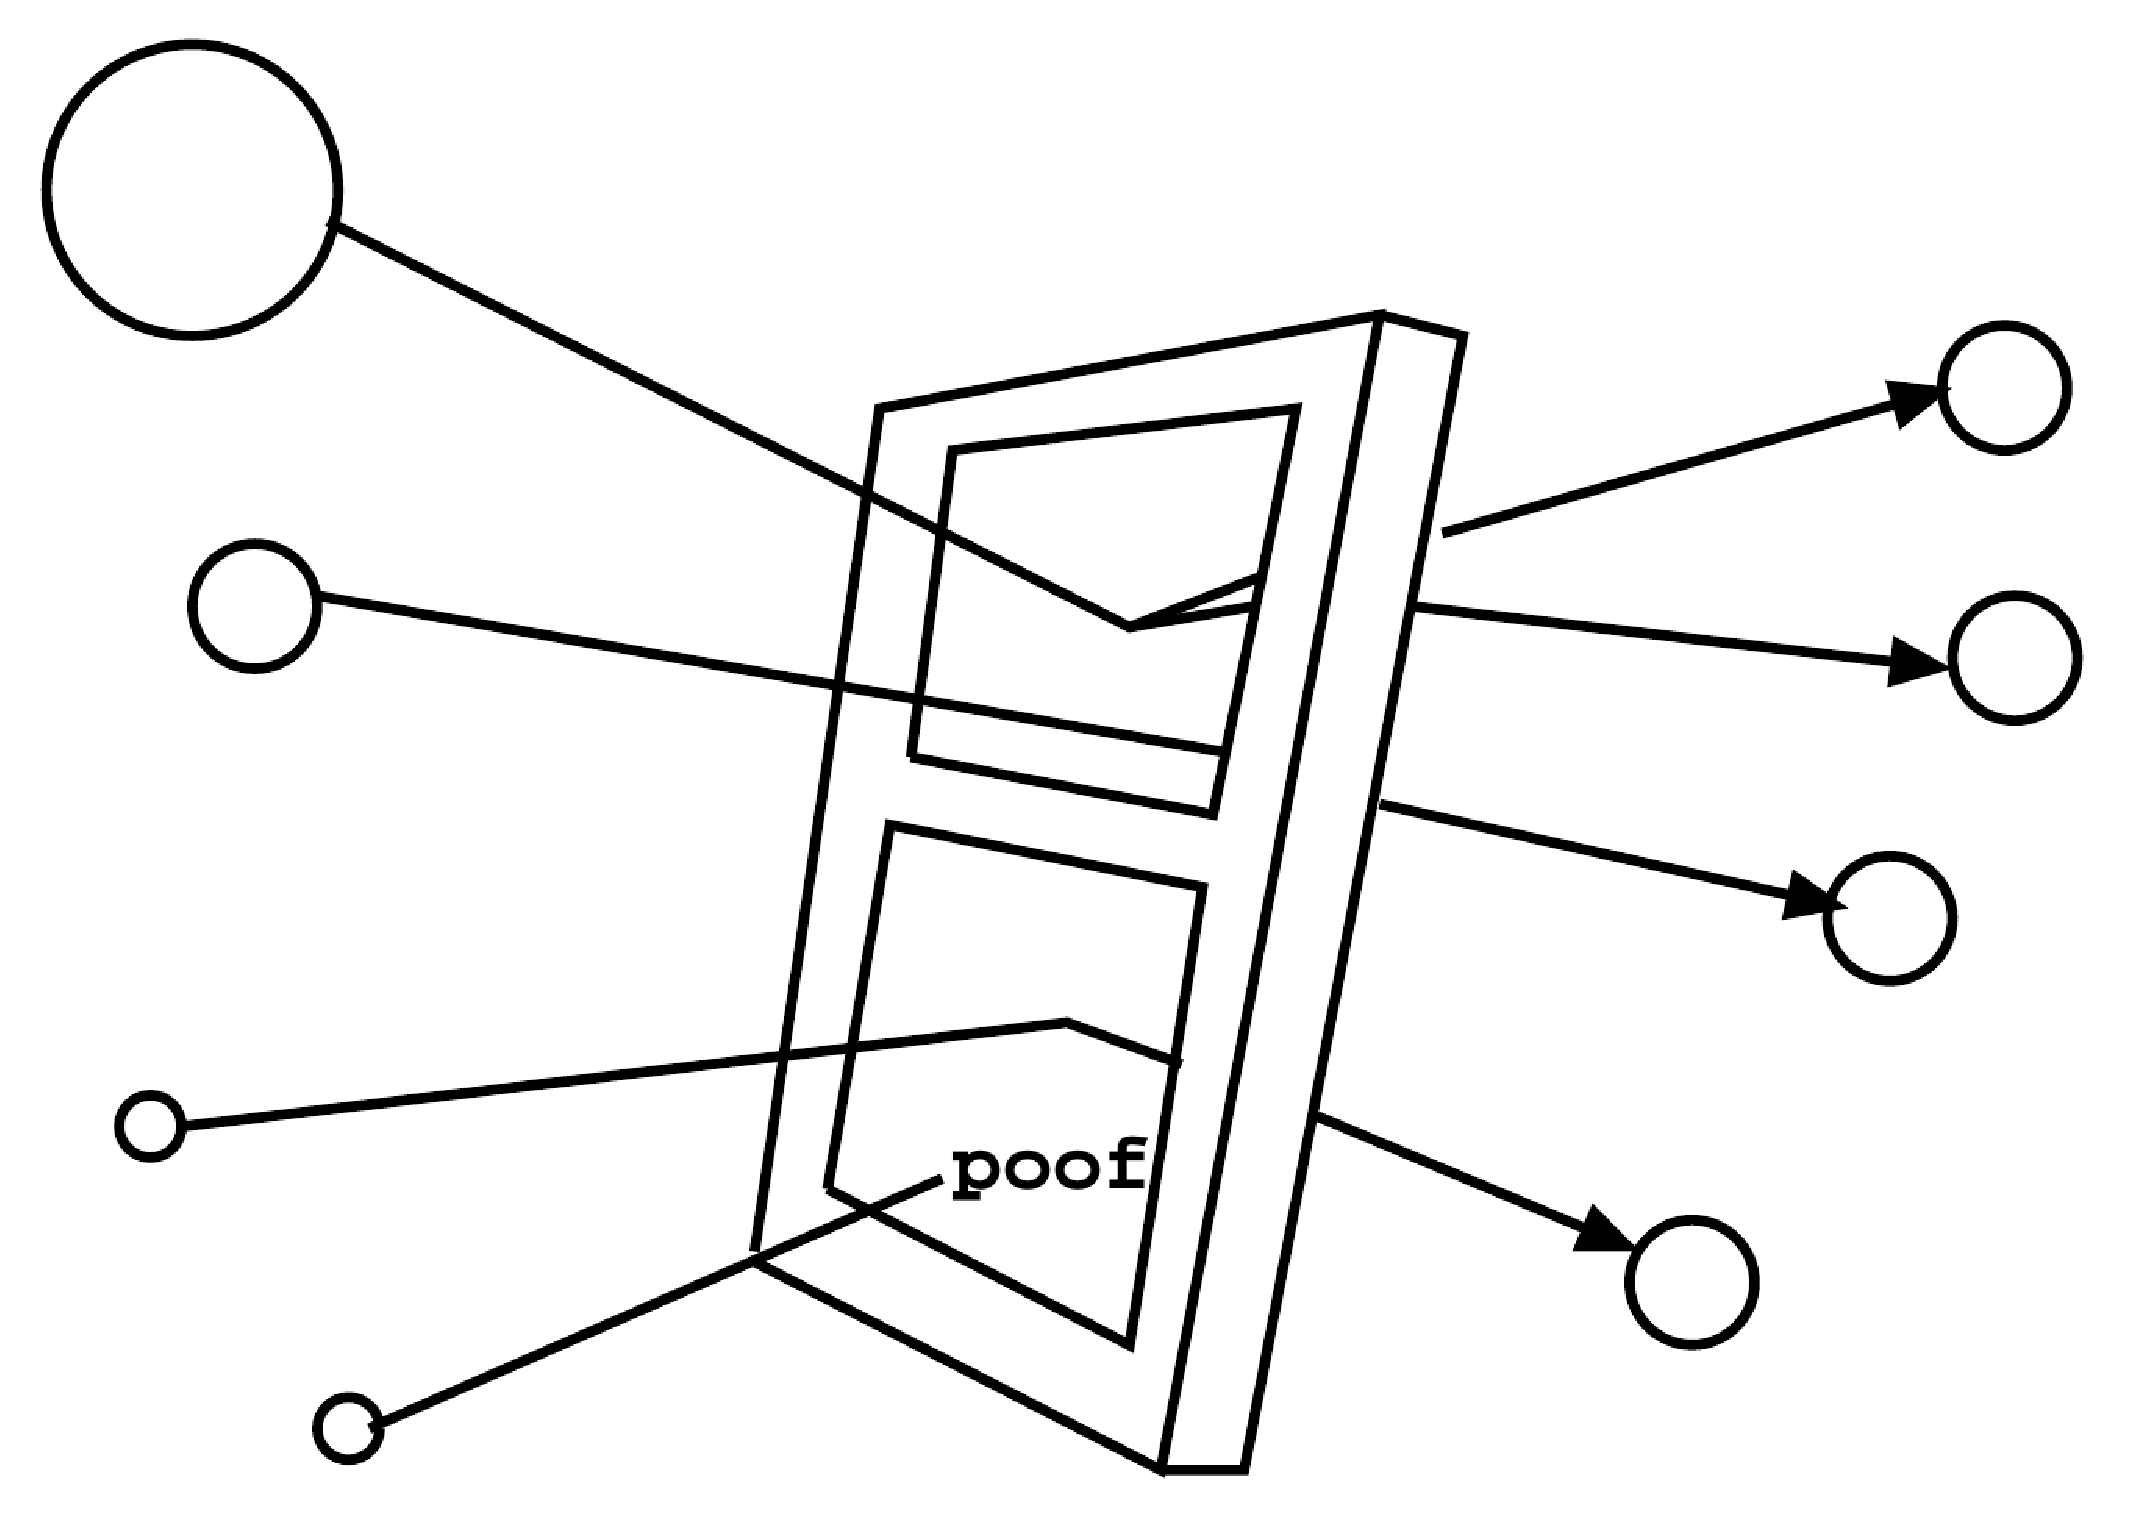
\includegraphics[width=0.85\textwidth]{img/ww-mcnp.eps}
\caption{Weight window phase space splitting and Russian roulette \cite{mcnp}.}
\label{fig:ww}
\end{figure}

The weight window may be used alone to good effect, but it is particularly powerful
when used in conjunction with other variance reduction techniques that introduce large
variations in particle weight. Well-specified weight windows keep the Monte Carlo 
solution from severe perturbations resulting from high-weight particles and 
simultaneously keep computational resources from wasting time on low-weight particles
by rouletting them.

\paragraph{Modified Sampling Methods}\mbox{} \\

Modified sampling methods alter the statistical sampling of a problem to increase the 
number of tallies per particle. For a given Monte Carlo event, it is possible to 
sample from an arbitrary distribution rather than the physical probability as long as 
the particle weights are adjusted to compensate. With modified sampling methods, 
sampling is done from distributions that send particles in desired directions or into 
other desired regions of phase space such as time or energy. Modified sampling methods
may also change the location or type of collisions. Categories of modified sampling
methods include implicit capture, forced collisions, and source biasing.

Using implicit capture (also called implicit absorption or survival biasing), 
particles are never killed by absorption. Instead, a particle's weight is reduced by
the absorption probability at each collision, allowing important particles to
survive by not being lost to absorption. Implicit capture can be thought of as a 
splitting process in which a particle of weight $w_0$ is split into two particles: one
of weight $w_0(1-\frac{\Sigma_a}{\Sigma_t})$ that survives and is 
subsequently followed, and one of weight $w_0\frac{\Sigma_a}{\Sigma_t}$ that is
instantaneously killed \cite{mcnp}.

The forced collision method increases sampling of collisions in specified spatial 
cells. Particles undergoing forced collisions are split into collided and uncollided
parts. The collided part of the particle is forced to react within the current cell,
while the uncollided part of the particle exits the cell without collision. When the
track of the uncollided particle portion is continued, it is followed with weight
$w_0e^{-\Sigma_t d}$, where $w_0$ is the original particle weight and $d$ is the
distance traveled between the splitting site and the cell boundary. The collided part
of the particle thus reacts with weight $w_0\left(1 - e^{-\Sigma_t d}\right)$. These
resultant weights are chosen to reflect the actual physics of the problem; 
$e^{-\Sigma_t d}$ is the probability of exiting the cell without collision, and 
$1 - e^{-\Sigma_t d}$ is the probability of colliding in the cell. One of these two
things must happen to the original particle of weight $w_0$, so we observe that the starting
weight is preserved.

Finally, particle sources may be biased with respect to one or more variables. This
allows for greater numbers of particles to be produced in more important ranges of 
each biased variable, with the particles' weights reduced accordingly. In the relevant
example of the neutron shielding problem, one may start more particles
at high energies and in strategic directions in order to get more particles to 
contribute to the desired solution. The corresponding weights of the particles are 
altered to correct the statistical distribution.

\subsection{Deterministic Methods}

In the case of deterministic methods, each of the six independent variables of the 
steady-state NTE is discretized, relevant boundary conditions are imposed, and the 
resulting system of linear algebraic equations is iterated over until an acceptable
solution has been reached. We limit the discussion here to the discretization of the
integro-differential form of the NTE and the finite-volume discrete ordinates method.

These discretizations introduce some errors into the calculations, with the
discretization of some variables being more problematic than others. For example, it
is functionally straightforward to discretize the energy and spatial variables, 
while discretizing angular space using the discrete ordinates method is more mathematically
intricate and often brings deleterious errors (``ray effects'') into problem solutions.
Deterministic methods may converge more quickly than Monte Carlo methods, especially
in the case of shielding problems, though the solutions are often plagued by the
aforementioned inaccuracies.

\subsubsection{Discretization of the Neutron Transport Equation}
\label{sec:disc}

\paragraph{Energy Discretization - The Multigroup Approximation}\mbox{} \\

Discretization of the energy variable is known as the ``multigroup'' approximation; 
it is relatively straightforward from a mathematical standpoint. Energy is broken up into $G$ 
groups, where the $g^{th}$ group has an upper bound of energy
$E_g$ and a lower bound of energy $E_{g+1}$ as shown in Figure \ref{egrid}. The highest energy 
group has $g = 0$ and the lowest energy group has $g = G-1$. This convention is used because 
neutrons are generally born at higher energies (starting in group 0 or 1) and scatter down to 
lower energies before undergoing an absorption reaction.

\begin{figure}[!thb]
\centering
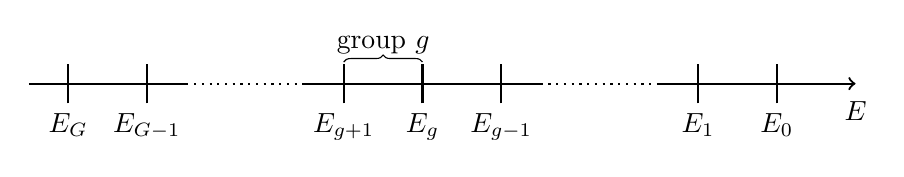
\begin{tikzpicture}
\draw[thick] (-5,0) -- (-3,0);
\draw[thick,dotted] (-3,0) -- (-1.5,0);
\draw[thick] (-1.5,0) -- (1.5,0);
\draw[thick,dotted] (1.5,0) -- (3,0);
\draw[thick,->] (3,0) -- (5.5,0);
\draw[thick] (-4.5,-0.25)--(-4.5,0.25);
\node [below] at (-4.5,-0.25) {$E_G$};
\draw[thick] (-3.5,-0.25)--(-3.5,0.25);
\node [below] at (-3.5,-0.25) {$E_{G-1}$};
\draw[thick] (-1,-0.25)--(-1,0.25);
\node [below] at (-1,-0.25) {$E_{g+1}$};
\draw[thick] (0,-0.25)--(0,0.25);
\node [below] at (0,-0.25) {$E_{g}$};
\node[above] at (-0.5, 0.25) {group $g$};
\draw[decorate,decoration={brace}](-1,0.275) -- (0,0.275);
\draw[thick] (1,-0.25)--(1,0.25);
\node [below] at (1,-0.25) {$E_{g-1}$};
\draw[thick] (3.5,-0.25)--(3.5,0.25);
\node [below] at (3.5,-0.25) {$E_1$};
\draw[thick] (4.5,-0.25)--(4.5,0.25);
\node [below] at (4.5,-0.25) {$E_0$};
\node [below] at (5.5,-0.1) {$E$};
\end{tikzpicture}
\caption{Discretized energy grid.}
\label{egrid}
\end{figure}

\FloatBarrier
Discretizing the NTE with respect to energy on this grid gives the $G$ multigroup
equations

\noindent\begin{minipage}{0.7\textwidth}
\begin{multline*}
\label{eq:mg_nte}
\bo \cdot \nabla \psi^g(\vecr,\bo) + \Sigma_t^g(\vecr) \psi^g(\vecr,\bo) =  \\
\sum_{g'=0}^{G-1}\int_{4\pi} \Sigma_s^{g'\rightarrow g}(\vecr,\bo'\cdot\bo)
\psi^{g'}(\vecr,\bo')d\bo' + Q^g(\vecr,\bo),
\end{multline*}
\end{minipage}
\hspace{-0.5cm}
\begin{minipage}{0.3\textwidth}
\begin{align}
\begin{split}
g &= 0,1,\ldots,G-1.
\end{split}
\end{align}
\end{minipage}
\vspace{0.1cm}

\noindent Here it is assumed that, within each energy group, the angular flux may be
approximated as the product of some known function of energy $f(E)$ and the group flux
$\psi^g(\vecr, \bo)$ as

\begin{equation}
\psi(\vecr,E,\bo) \approx f(E)\psi^g(\vecr,\bo), \quad E_{g+1} < E \leq E_{g}\:,
\end{equation}

\noindent where $f(E)$ is normalized such that $\int_{E_g+1}^{E_{g}}f(E)dE = 1$. With 
this, the multigroup cross sections and the group source are similarly defined
\cite{lm} as

\begin{align}
\Sigma_t^g(\vecr) &= \int_{E_{g+1}}^{E_{g}}\Sigma_t(\vecr,E)f(E)dE, \\
\Sigma_s^{g'\rightarrow g}(\vecr,\bo'\cdot\bo) &= \int_{E_{g+1}}^{E_{g}}\int_{E_{g'+1}}^{E_{g'}}
\Sigma_s(\vecr, E'\rightarrow E, \bo'\cdot\bo)f(E')dE'dE, \\
Q^g(\vecr,\bo) &= \int_{E_{g+1}}^{E_{g}}Q(\vecr,E,\bo)dE.
\end{align}

\paragraph{Spatial Discretization}\mbox{} \\

In the interest of completeness, we will briefly discuss the discretization of space.
The LDO equations are inherently three-dimensional \cite{ahrens}, so we will restrict
the discussion to three-dimensional space with point positions specified by Cartesian
coordinates. A general mesh cell is shown in Figure \ref{fig:spatial_mesh}.

\begin{figure}[!htb]
\centering
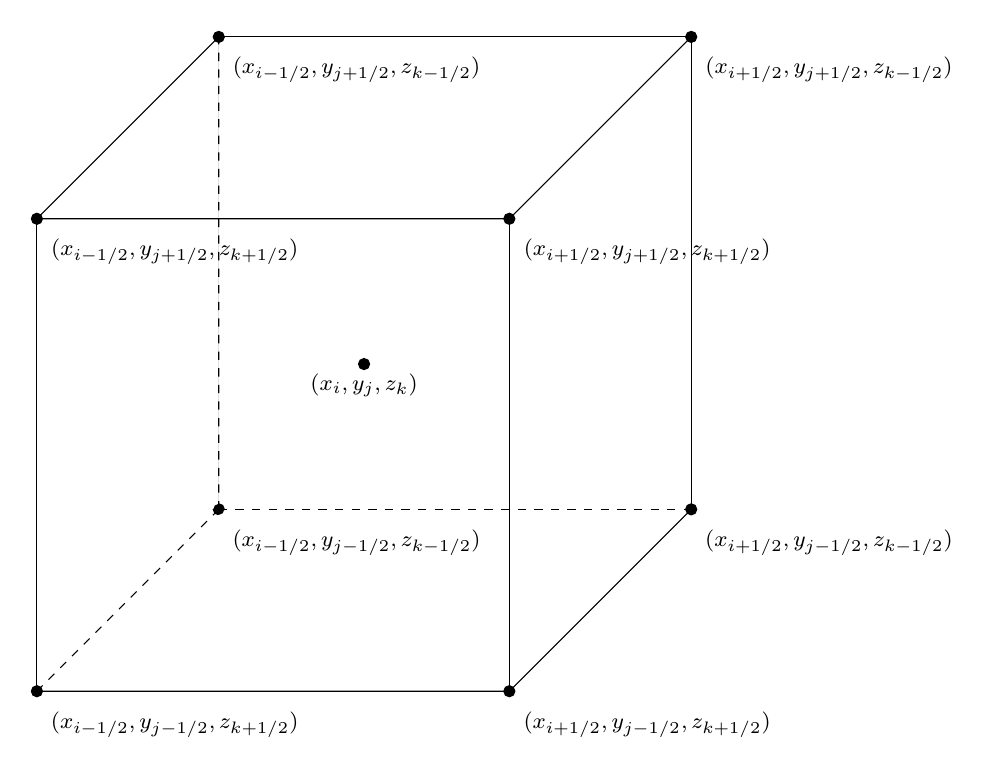
\begin{tikzpicture}
\filldraw (xyz cs:x=-3,y=-3,z=3) circle (2pt) node {} -- 
          (xyz cs:x=3,y=-3,z=3) circle (2pt) node {};
\node[fill,circle,inner sep=0pt, minimum size = 2pt,
      label={[shift={(1.75,-0.75)}]
      \footnotesize$(x_{i-1/2}, y_{j-1/2}, z_{k+1/2})$}] 
      at (xyz cs:x=-3,y=-3,z=3) {};
\node[fill,circle,inner sep=0pt, minimum size = 2pt,
      label={[shift={(1.75,-0.75)}]
      \footnotesize$(x_{i+1/2}, y_{j-1/2}, z_{k+1/2})$}] 
      at (xyz cs:x=3,y=-3,z=3) {};
\filldraw (xyz cs:x=-3,y=3,z=3) circle (2pt) node {} -- 
          (xyz cs:x=3,y=3,z=3) circle (2pt) node {};
\node[fill,circle,inner sep=0pt, minimum size = 2pt,
      label={[shift={(1.75,-0.75)}]
      \footnotesize$(x_{i-1/2}, y_{j+1/2}, z_{k+1/2})$}] 
      at (xyz cs:x=-3,y=3,z=3) {};
\node[fill,circle,inner sep=0pt, minimum size = 2pt,
      label={[shift={(1.75,-0.75)}]
      \footnotesize$(x_{i+1/2}, y_{j+1/2}, z_{k+1/2})$}] 
      at (xyz cs:x=3,y=3,z=3) {};
\filldraw (xyz cs:x=-3,y=3,z=3) -- 
          (xyz cs:x=-3,y=3,z=-3) circle (2pt) node[] {};
\node[fill,circle,inner sep=0pt, minimum size = 2pt,
      label={[shift={(1.75,-0.75)}]
      \footnotesize$(x_{i-1/2}, y_{j+1/2}, z_{k-1/2})$}] 
      at (xyz cs:x=-3,y=3,z=-3) {};
\filldraw (xyz cs:x=3,y=3,z=3)  -- 
          (xyz cs:x=3,y=3,z=-3) circle (2pt) node {};
\node[fill,circle,inner sep=0pt, minimum size = 2pt,
      label={[shift={(1.75,-0.75)}]
      \footnotesize$(x_{i+1/2}, y_{j+1/2}, z_{k-1/2})$}] 
      at (xyz cs:x=3,y=3,z=-3) {};
\filldraw (xyz cs:x=3,y=-3,z=3) -- 
          (xyz cs:x=3,y=-3,z=-3) circle (2pt) node {};
\node[fill,circle,inner sep=0pt, minimum size = 2pt,
      label={[shift={(1.75,-0.75)}]
      \footnotesize$(x_{i+1/2}, y_{j-1/2}, z_{k-1/2})$}]
      at (xyz cs:x=3,y=-3,z=-3) {};
\draw (xyz cs:x=-3,y=-3,z=3) -- (xyz cs:x=-3,y=3,z=3);
\draw (xyz cs:x=3,y=-3,z=3) -- (xyz cs:x=3,y=3,z=3);
\draw (xyz cs:x=-3,y=3,z=-3) -- (xyz cs:x=3,y=3,z=-3);
\draw (xyz cs:x=3,y=-3,z=-3) -- (xyz cs:x=3,y=3,z=-3);
\node[fill,circle,inner sep=0pt, minimum size = 2pt,
      label={[shift={(1.75,-0.75)}]
      \footnotesize$(x_{i-1/2}, y_{j-1/2}, z_{k-1/2})$}] 
      at (xyz cs:x=-3,y=-3,z=-3) {};
\filldraw[dashed] (xyz cs:x=-3,y=-3,z=-3) circle (2pt) node {} -- 
                  (xyz cs:x=-3,y=3,z=-3);
\draw[dashed] (xyz cs:x=-3,y=-3,z=-3) -- (xyz cs:x=3,y=-3,z=-3);
\draw[dashed] (xyz cs:x=-3,y=-3,z=-3) -- (xyz cs:x=-3,y=-3,z=3);
\filldraw (xyz cs: x=0,y=0,z=0) circle (2pt) node[below] 
          {\footnotesize$(x_i, y_j, z_k)$};
\end{tikzpicture}
\caption{General three-dimensional mesh cell \cite{exmm}.}
\label{fig:spatial_mesh}
\end{figure}

The mesh cell is centered at the $i^{th}$ position along the $x$-axis, the $j^{th}$
position along the $y$-axis, and the  $k^{th}$ position along the $z$-axis. Indexing
is such that there are $I$ mesh cells with $I+1$ grid points in the $x$-direction, $J$ mesh
cells with $J+1$ grid points in the $y$-direction, and $K$ mesh cells with $K+1$ grid points in 
the $z$-direction. It is assumed that all material 
properties are constant within a given cell. In order to eventually solve for the 
scalar flux in a given system, we are interested in solving for the angular flux at 
the center of each mesh cell, resulting in the $G\times I \times J \times K$
equations shown in Equation \ref{eq:mg_xyz_nte}.

\begin{minipage}{0.65\textwidth}
\begin{multline*}
\label{eq:mg_xyz_nte}
\bo\cdot\nabla\psi^g_{i,j,k}(\bo)+\Sigma_{t,i,j,k}^g\psi^g_{i,j,k}(\bo) =  \\
\sum_{g'=0}^{G-1}\int_{4\pi} \Sigma_{s,i,j,k}^{g'\rightarrow g}(\bo'\cdot\bo)
\psi^{g'}_{i,j,k}(\bo')d\bo' + Q^g_{i,j,k}(\bo),
\end{multline*}
\end{minipage}
\begin{minipage}{0.31\textwidth}
\begin{align}
\begin{split}
g &= 0,1,\ldots,G-1,\\
i &= 1,2,\ldots,I,\\
j &= 1,2,\ldots,J,\\
k &= 1,2,\ldots,K.
\end{split}
\end{align}
\end{minipage} \strut

\noindent To solve for these cell-centered flux 
quantities in practice, auxiliary equations are introduced. As these are specific to the 
spatial discretization employed in a given solution and do not differ between the classical
discrete ordinates equations and the LDO formulation, we refer the reader to Reference
\cite{denovo} for more detail on spatial differencing and solution methods.

\paragraph{Angular Discretization - Discrete Ordinates}\mbox{} \\
\label{sec:do}

The last part of phase space to discretize in the time-independent NTE is angle.
The discrete ordinates method is the most common angular discretization method
incorporated into general-purpose neutron transport codes \cite{lm}. It is a 
collocation method that requires the solution of the NTE to be exact at a 
distinct number of angles $\bo_n$:

\noindent\begin{minipage}{0.69\textwidth}
\begin{align*}
\bo_n&\cdot\nabla\psi^{g,n}_{i,j,k}+\Sigma_{t,i,j,k}^g\psi^{g,n}_{i,j,k} = \\
&\sum_{g'=0}^{G-1}\sum_{\ell=0}^P \Sigma_{s,\ell,i,j,k}^{g'\rightarrow g}
\bigg[\Ye{\ell 0}{n}\phi_{\ell 0}^{g'} + \sum_{m=1}^{\ell}
\bigg(\Ye{\ell m}{n}\phi_{\ell m}^{g'} \\
&\qquad\qquad\qquad\qquad\qquad\qquad
 + \Yo{\ell m}{n}\vartheta_{\ell m}^{g'}\bigg)\bigg]
 + Q^{g,n}_{i,j,k},
\end{align*}
\end{minipage}
\hspace{-0.55cm}
\begin{minipage}{0.31\textwidth}
\begin{align}
\begin{split}
g &= 0,1,\ldots,G-1,\\
i &= 1,2,\ldots,I,\\
j &= 1,2,\ldots,J,\\
k &= 1,2,\ldots,K,\\
n &= 1,2,\ldots,N.
\label{eq:do}
\end{split}
\end{align}
\end{minipage}
\vspace{0.1cm}

\noindent Here, $\psi^n \equiv \psi(\bo_n)$ and the angles are integrated by a
quadrature rule such that their corresponding weights $w_n$ sum to $4\pi$. Weights and
ordinates (``quadrature sets'') are chosen in such a way as to provide good 
approximations to angular integrals used to evaluate scalar flux \cite{lm,exmm}. The 
upper limit of summation for the scattering term spherical harmonic expansion, denoted
as $P$ in Equation \ref{eq:do}, is known as the ``\pn order''. The scattering cross section
coefficient values $\Sigma_{s,\ell,i,j,k}^{g'\rightarrow g}$ come from data libraries based on
experimental measurements.

The scattering source is expanded in terms of spherical harmonics:

\begin{equation}
\phi_{\ell,i,j,k}^{g}=\sum_{n=1}^N \Ye{\ell m}{n}w_n\psi^{g,n}_{i,j,k}\ \text{ and }\
\vartheta_{\ell,i,j,k}^{g} = \sum_{n=1}^N \Yo{\ell m}{n}w_n\psi^{g,n}_{i,j,k},
\label{sph_harm_exp}
\end{equation}

\noindent where $\phi$ and $\vartheta$ are
referred to as the ``flux moments''. 
Here, $\Ye{\ell m}{n}$ and $\Yo{\ell m}{n}$ are the ``even'' and ``odd'' 
real components of the spherical harmonic functions, defined as \cite{exmm}

\begin{equation}
\Ye{\ell m}{n} = (-1)^m\sqrt{(2-\delta_{m0})\frac{2\ell+1}{4\pi}
                       \frac{(\ell-m)!}{(\ell+m)!}}
                       P_{\ell m}(\cos\theta)\cos(m\varphi),
\label{eq:sph_e}
\end{equation}
\begin{equation}
\Yo{\ell m}{n} = (-1)^m\sqrt{(2-\delta_{m0})\frac{2\ell+1}{4\pi}
                       \frac{(\ell-m)!}{(\ell+m)!}}
                       P_{\ell m}(\cos\theta)\sin(m\varphi).
\label{eq:sph_o}
\end{equation}

\noindent In Equations \ref{eq:sph_e} and \ref{eq:sph_o}, $P_{\ell m}(\cos\theta)$ is 
the associated Legendre polynomial and $(\theta,\varphi)$ are the components of $\bo$ 
as shown in Figure \ref{fig:ang} and Equations \ref{eq:ang_disc} -- \ref{eq:ang_sum}. It is
assumed that the double differential scattering cross section depends only on the dot product of
the incoming and outgoing angles of the particle undergoing scattering.

To summarize Equations 
\ref{eq:do} -- \ref{eq:sph_o}, we note that the double differential scattering cross section is
expanded into the real components of the spherical harmonic functions, which can be represented
with Legendre polynomials; these are then multiplied with the angular flux moments expanded into
spherical harmonic functions.

\begin{figure}[!hbt]
\begin{minipage}{0.5\textwidth}
\begin{tikzpicture}
\coordinate (origin) at (0,0,0);
\coordinate (omega) at (2,4,7);
\coordinate (xaxis) at (0,0,9);
\coordinate (yaxis) at (3,0,0);
\coordinate (diag) at (2,5,0);
% axes
\draw[thick,->] (xyz cs:x=0) -- (xyz cs:x=3) node[right] {$x$};
\draw[thick,->] (xyz cs:y=0) -- (xyz cs:y=5) node[above] {$y$};
\draw[thick,->] (xyz cs:z=0) -- (xyz cs:z=8) node[below] {$z$};
% dashed box lines
\draw[dashed] (xyz cs:z=7,y=4) -- (xyz cs:z=7,y=0.25) node[left] {$\xi$};
\draw[dashed] (xyz cs:z=7,y=0) -- (xyz cs:z=7,x=2);
\draw[dashed] (xyz cs:z=7,x=2) -- (xyz cs:z=7,y=4,x=2);
\draw[dashed] (xyz cs:z=7,y=4,x=0) -- (xyz cs:z=7,y=4,x=2);

\draw[dashed] (xyz cs:x=2,z=0) -- (xyz cs:x=2,z=7);
\draw[dashed] (xyz cs:x=2,z=0,y=4) -- (xyz cs:x=2,z=0); 
\draw[] (xyz cs:x=2.3,y=-0.1,z=0) -- (xyz cs:x=2.3,y=-0.1,z=0) node[above] {$\mu$};
\draw[dashed] (xyz cs:x=2,z=0,y=4) -- (xyz cs:x=0,z=0,y=4) node[left] {$\eta$}; 
\draw[dashed] (xyz cs:x=0,z=0,y=4) -- (xyz cs:z=7,y=4);
\draw[dashed] (xyz cs:x=2,z=0,y=4) -- (xyz cs:z=7,y=4,x=2);

\draw[thick,->] (xyz cs:x=0,y=0,z=0) -- (xyz cs:x=2,z=7,y=4);
\draw[] (xyz cs:x=2,z=7,y=4) -- (xyz cs:x=2,z=7,y=4) node[above] {$\bo$};
\draw[dashed] (xyz cs:x=2,z=0,y=4) -- (xyz cs:x=0,z=0);
\draw[dashed] (xyz cs:z=7,y=0) -- (xyz cs:x=2,z=7,y=4);

\pic [draw,<-,angle radius=0.3cm,angle eccentricity=1.4,"$\theta$"]
     {angle = omega--origin--xaxis};
\pic [draw,->,angle radius=0.5cm,angle eccentricity=1.4,"$\varphi$"]
     {angle = yaxis--origin--diag};
\end{tikzpicture}
\caption{Angular coordinate system \cite{exmm}.}
\label{fig:ang}
\end{minipage}
\begin{minipage}{0.5\textwidth}
\begin{subequations}
\begin{align}
\label{eq:ang_disc}
&\xi = \cos\theta \\
&\mu = \sqrt{1-\xi^2}\cos\varphi \\
&\eta = \sqrt{1-\xi^2}\sin\varphi
\end{align}
\end{subequations}
\begin{equation}
\label{eq:ang_sum}
\mu^2 + \eta^2 + \xi^2 = 1
\end{equation}
\end{minipage}
\end{figure}

\FloatBarrier Commonly-used quadrature sets include level-symmetric, Gauss-
Legendre product, quadruple range (QR) product, and linear-discontinuous
finite element (LDFE). The various quadrature set types have different
properties with each being better for certain classes of problems. For
example, relatively coarse (sixteen angles per octant) QR product quadratures
are generally sufficient for generating variance reduction parameters for
neutron transport problems, but more finely resolved quadrature sets are
recommended for photon transport problems \cite{advantg}. Level-symmetric
quadrature sets are widely applied for general applications \cite{lm} but
tend to exhibit far more ray effects than QR product quadratures
\cite{advantg}. In the following subsection, we will discuss ray effects in
greater detail.

\subsubsection{Ray Effects}
\label{sec:ray}

Ray effects are unphysical computational anomalies in the scalar flux solution that 
arise from the discrete ordinates formulation. Because the NTE is only evaluated  
 at a finite number of discrete angles, the number of directions in 
which particles may stream is restricted. As a consequence of this, contributions to 
the scalar flux from uncollided particles are limited to those from the discrete 
angles along which particle sources are ``visible'' \cite{lathrop}. A demonstrative
example of ray effects is shown in Figure \ref{fig:ray}. The plot shows results from 
the PARTISN \cite{partisn} code using a triangular $P_n - T_n$ quadrature with
48 points and a
scattering ratio of $c = 0.25$ \cite{ahrens}. Although the point source
emits neutrons isotropically, the scalar flux calculated at a given radius out from 
the source sees contributions only from the discrete angles along which particles may
stream. That is, the flux at a given distance from the point source is actually equal 
in all directions and so the figure should appear to be a sphere, but the discrete
angles restrict streaming pathways to the rays shown in the image. 

\begin{figure}[!htb]
\centering

\includegraphics[width=0.5\textwidth]{img/ray-effects.png}
\caption{Isosurface plot of scalar flux from a point source \cite{ahrens}.}
\label{fig:ray}
\end{figure}

The severity of ray effects in a given simulation depends on the properties of
the  sources. The largest consequences tend to occur in scenarios with localized
sources and relatively minimal scattering. When using the discrete ordinates
approximation in a purely absorbing medium, regardless of the accuracy of the
angular flux calculations and the number of discrete angles used, it is always
possible to get far enough away from a localized source such that a poor value
of the scalar flux is obtained at that point \cite{lathrop}. In a scattering
medium with localized sources, angular flux values are incorrect because they
depend  on integrals that are poorly approximated by the quadrature formulation.
In contrast  to this, neutrons exiting scattering reactions are generally less
localized and  consequently tend to  mitigate ray effects. As we will see later
in the chapter, one key point of interest in using the LDO equations as part of
a hybrid method calculation is that the LDO equations mitigate ray effects when
higher-order quadrature sets are used  \cite{ahrens}.

\subsection{Hybrid Methods}

Hybrid methods aim to combine the previously described Monte Carlo
methods and deterministic methods in such a way as to perform calculations that result
in statistically meaningful results within a tractable period of computation time.
Generally, these hybrid methods are implemented such that the solution(s) from a 
deterministic code are used to inform a Monte Carlo code. When this is done well, the
Monte Carlo code converges more quickly than without the information from the
deterministic solution(s).

Specifically, an adjoint and/or forward flux solution generated by a deterministic 
transport solver is used to make a weight window map for a Monte Carlo run. As was
noted earlier, weight windows are most effective when specified well and when used in
conjunction with other variance reduction techniques. Because developing effective
weight window maps can be labor-intensive and require a user to have significant 
\textit{a priori} knowledge about the problem being solved, automated hybrid methods
have been developed to couple deterministic solutions to Monte Carlo transport
calculations.

\section{Previous Work}

Substantial effort has been placed into the development and automated execution of
hybrid methods. This section will discuss previous work in this field with a 
particular emphasis on the present state of hybrid methods as well as hybrid methods 
that incorporate neutron direction of travel.

Here we begin by describing the CADIS (consistent adjoint driven importance sampling)
and \fwc\ (forward-weighted consistent adjoint driven importance sampling) methods, 
which are the current state
of the art of Monte Carlo variance reduction parameter generation. These are 
introduced first because, as will be described in more detail later, this work 
employs solutions of the LDO equations in combination with the CADIS and \fwc\ 
methods via the ADVANTG software. Following this, we present a discussion of selected 
work in angle-informed hybrid methods, focusing on variants of CADIS and \fwc.

\subsection{CADIS and FW-CADIS}

\subsubsection{CADIS}
\label{sec:cadis}

The CADIS method was introduced by Wagner and Haghighat in 1997 to automate Monte 
Carlo variance reduction parameter generation \cite{cadis}. CADIS is based on the 
source biasing and weight window techniques described above, does not depend heavily 
on user experience, and was implemented as described in Reference \cite{cadis} in the 
MCNP \cite{mcnp} code. Most importantly, the CADIS method produces source biasing 
parameters and weight window target values such that particles are born with the target
weights. Since CADIS is used heavily in this work, it is pertinent to 
describe the theory behind the method.

The goal of most Monte Carlo neutron transport problems is to calculate some response
(scalar flux, dose, etc.) at some location in phase-space. This can be posed as 
solving the following integral equation:

\begin{equation}
R = \int_P \psi(P)\sigma_d(P)dP,
\label{eq:cadis_r1}
\end{equation}

\noindent where $R$ is the response of interest, $\psi$ is the neutron angular flux,
and $\sigma_d$ is some objective function in the phase-space $(\vecr, E, \bo) \in P$.
We now introduce the adjoint identity

\begin{equation} 
\langle \psi^{\dagger}, H\psi\rangle=\langle\psi , H^{\dagger}\psi^{\dagger}\rangle
\label{eq:adj}
\end{equation}

\noindent where $H$ is the transport operator and the dagger superscript indicates an 
adjoint quantity. Using Equation \ref{eq:adj} and some algebraic manipulations, it 
can be shown that

\begin{equation}
R = \int_P \psi^{\dagger}(P)q(P)dP,
\label{eq:cadis_r2}
\end{equation}

\noindent where $\psi^{\dagger}$ and $q$ are the adjoint neutron angular flux function
and the particle source density, respectively. For a given problem with a vacuum 
boundary condition, Equations \ref{eq:cadis_r1} and \ref{eq:cadis_r2} are equivalent 
expressions for $R$. The adjoint neutron angular flux function $\psi^{\dagger}$ has 
physical meaning as the expected contribution to the response $R$ from a particle in 
phase-space $P$. In other words, the adjoint flux function is significant because it 
represents the importance of those source particles to the response of interest.

To calculate the response with the Monte Carlo method, the independent variables are
sampled from the probability density function (PDF) $q(P)$. However, this may not be
the best PDF from which to sample, so an alternative PDF $\qhat(P)$ can be introduced
into the integral:

\begin{equation}
R = \int_P \left[\frac{\psi^{\dagger}(P)q(P)}{\qhat(P)}\right]\qhat(P)dP,
\end{equation}

\noindent where $\qhat(P) \geq 0$ and the integral of $\qhat(P)$ over $P$ is 
normalized to unity. Then, the alternative PDF $\qhat(P)$ that will minimize the 
variance of the response is given by

\begin{equation}
\qhat(P) = \frac{\psi^{\dagger}(P)q(P)}{\int_P\psi^{\dagger}(P)q(P)dP}.
\label{eq:qhat}
\end{equation}

\noindent Looking at Equation \ref{eq:qhat}, we see that the numerator is the 
response from phase-space $P$ and the denominator is the total response $R$. Thus, 
this definition of $\qhat(P)$ is a measure of the contribution from phase-space $P$ 
to the response. It is useful to bias the sampling of source particles by this ratio 
of their contribution to the detector response.

Because the source variables are sampled from this new biased PDF, the statistical
weight of the source particles must be corrected such that

\begin{equation}
w(P)\qhat(P) = w_0q(P),
\label{eq:cadis_w1}
\end{equation}

\noindent where $w_0$ is the unbiased particle starting weight and is set equal to 1.
Substituting Equation \ref{eq:qhat} into Equation \ref{eq:cadis_w1} and solving for 
$w(P)$ gives the following expression for the statistical weight of the particles:

\begin{equation}
w(P) = \frac{\int_P\psi^{\dagger}(P)q(P)dP}{\psi^{\dagger}(P)}
= \frac{R}{\psi^{\dagger}(P)}.
\label{eq:cadis_w2}
\end{equation}

\noindent Equation \ref{eq:cadis_w2} demonstrates an inverse relationship between 
this adjoint (importance) function and the statistical particle weight. 

Now, let us consider the
transport process in this context. The integral transport equation for particle
density in the phase-space $P$ is given by

\begin{equation}
\psi(P) = \int K(P'\rightarrow P)\psi(P')dP' + q(P)
\label{eq:cadis_nte1}
\end{equation}

\noindent where $K(P'\rightarrow P)$ is the expected number of particles entering $dP$
about $P$ from an event in $P'$. Given the preceding discussion, we would like to 
transform Equation \ref{eq:cadis_nte1} to be in terms of the biased source 
distribution $\qhat(P)$. Defining

\begin{equation}
\psihat(P) = \frac{\psi(P)\psi^{\dagger}(P)}{\int \psi^{\dagger}(P)q(P)dP},
\end{equation}

\noindent we can write Equation \ref{eq:cadis_nte1} in terms of $\qhat(P)$ as

\begin{equation}
\psihat(P) = \frac{\psi^{\dagger}(P)}{\int \psi^{\dagger}(P)q(P)dP}
\int K(P'\rightarrow P)\psi(P')dP' + \qhat(P).
\label{eq:cadis_nte2}
\end{equation}

\noindent Equation \ref{eq:cadis_nte2} can also be written as

\begin{equation}
\psihat(P) = \int K(P'\rightarrow P)\psihat(P')
\left[\frac{\psi^{\dagger}(P)}{\psi^{\dagger}(P')}\right]dP' + \qhat(P)\:,
\end{equation}

\noindent which allows us to define

\begin{equation}
\khat(P' \rightarrow P) = K(P'\rightarrow P)
\left[\frac{\psi^{\dagger}(P)}{\psi^{\dagger}(P')}\right]
\end{equation}

\noindent and finally write

\begin{equation}
\psihat(P) = \int\khat(P' \rightarrow P)\psihat(P')dP' +\qhat(P).
\end{equation}

Because $K(P'\rightarrow P)$ is unknown, we simulate neutron transport in the usual
unbiased way and change the number of particles emerging in $P$ from an event in
$P'$ by the ratio of importances $\psi^{\dagger}(P)/\psi^{\dagger}(P')$. When this
ratio is above one, splitting occurs, and rouletting occurs when the ratio is less 
than one. The statistical weights of the particles resulting from splitting and/or
rouletting are then corrected such that

\begin{equation}
w(P)K(P' \rightarrow P)\left[\frac{\psi^{\dagger}(P)}{\psi^{\dagger}(P')}\right] = 
w(P')K(P' \rightarrow P)
\end{equation}

\noindent or

\begin{equation}
w(P) = w(P')\left[\frac{\psi^{\dagger}(P)}{\psi^{\dagger}(P')}\right].
\label{eq:cadis_w3}
\end{equation}

\noindent With this, reduced variance can be achieved when all source and transport
sampling is proportional to its importance. The source particles' energy and position
are sampled from the biased source distribution

\begin{equation}
\qhat(\vecr,E) = 
\frac{\phi^{\dagger}(\vecr,E)q(\vecr,E)}
{\int_V\int_E\phi^{\dagger}(\vecr,E)q(\vecr,E) dE\ d\vecr} 
= \frac{\phi^{\dagger}(\vecr,E)q(\vecr,E)}{R}.
\label{eq:cadis_sb}
\end{equation}

\noindent Here, the physical meaning of the numerator is the detector response from
space-energy element $(d\vecr,dE)$ and the denominator is the total detector response
$R$. As in the preceding derivation, this ratio is a measure of the particles' 
relative contribution to the detector response.

To bias particles undergoing the transport process, the weight window technique is 
applied. Weight window lower bounds $w_{\ell}$ must be calculated such that the
statistical weights defined in Equation \ref{eq:cadis_w2} fall at the center of the
weight window intervals. The width of a given interval is denoted by 
$c_u = w_u/w_{\ell}$, the ratio of upper and lower weight window values. The
weight window lower bounds are then given by

\begin{equation}
w_{\ell}(\vecr,E) = \frac{w}{\left(\frac{c_u +1}{2}\right)} 
= \frac{R}{\phi^{\dagger}(\vecr,E)}\frac{1}{\left(\frac{c_u +1}{2}\right)}.
\label{eq:cadis_tb}
\end{equation}

\noindent Using this definition, the weight window technique then performs particle
splitting and/or rouletting consistent with the statistical weight given in Equation
\ref{eq:cadis_w3}.

The key result of the foregoing discussion is that the statistical weights of the
source particles are within the bounds of the weight windows. In other words, the
source-biasing parameters and the weight window target values are consistent. This
circumvents the potential of particles being immediately split or rouletted upon birth
and avoids the resultant degradation in computational efficiency. We refer the reader
to Reference \cite{cadis} for a complete discussion of results and analysis of the initial
implementation of the CADIS method.

Note that Equations \ref{eq:cadis_sb} and \ref{eq:cadis_tb} use the scalar adjoint 
flux rather than the angular flux. This is consistent with the
original implementation of the CADIS method in MCNP as well as the implementation of
the method in ADVANTG; the scalar adjoint neutron flux function is used in both tools
\cite{cadis, advantg}. Historically, this was done to reduce the memory required for
the deterministic calculation as well as the weight window map. Additionally, the 
angular adjoint flux resulting from an \sn calculation was not considered to be 
sufficiently accurate due to the limited number of discrete angles used for the 
calculation. Further, people have
generally not developed weight windows that are a function of angle.

The CADIS method is very effective for automated optimization of localized detectors
but falls short of efficiently optimizing distributed responses. FW-CADIS, discussed 
in the next section, was developed to address this issue.

\subsubsection{FW-CADIS}
\label{sec:fwcadis}

FW-CADIS, introduced
by Wagner, Blakeman, and Peplow in 2009, is a variation on the CADIS method to 
increase the efficiency of Monte Carlo calculations of distributions and responses at 
multiple localized detectors \cite{fwcadis}.

For this global variance reduction method, a response with uniformly-low statistical 
uncertainty across all phase-space is desired. One way to target this for a given 
Monte Carlo simulation is to uniformly distribute the particles throughout the system.
Though this is not a physical response, it is a proxy for the goal of obtaining 
uniform uncertainty. It also indicates the possibility of developing an adjoint 
importance function that represents the importance of particles to achieving the goal
of uniform particle distribution.

With this new problem formulation, the problem of calculating particle density is cast
into the response formulation:

\begin{equation}
R = \int_{4\pi}\int_{V}\int_{E}\psi(\vecr,E,\bo)f(\vecr,E,\bo)dE\ dV\ d\bo,
\end{equation}

\noindent where $f(\vecr,E,\bo)$ is some function that converts angular neutron flux 
to Monte Carlo particle density. Recall that the angular neutron flux can be defined 
as the product of the physical particle density $n$ and velocity $v$:

\begin{equation}
\psi(\vecr,E,\bo) = n(\vecr,E,\bo)v(\vecr,E,\bo)
\label{eq:psi}
\end{equation}

\noindent and the physical particle density is related to the Monte Carlo particle 
density $m$ and the average particle weight $\bar{w}$ by

\begin{equation}
n(\vecr,E,\bo) = \bar{w}(\vecr,E,\bo)m(\vecr,E,\bo).
\label{eq:dens}
\end{equation}

\noindent Using Equations \ref{eq:psi} and \ref{eq:dens}, the Monte Carlo particle 
density can be estimated by

\begin{equation}
m(\vecr,E,\bo) = \frac{n(\vecr,E,\bo)}{\bar{w}(\vecr,E,\bo)} 
= \frac{\psi(\vecr,E,\bo)}{\bar{w}(\vecr,E,\bo)v(\vecr,E,\bo)}
\end{equation}

\noindent and the total Monte Carlo density can be estimated by

\begin{equation}
R = \int_{4\pi}\int_{V}\int_{E}\psi(\vecr,E,\bo)
\left[\frac{1}{\bar{w}(\vecr,E,\bo)v(\vecr,E,\bo)}\right]dE\ dV\ d\bo.
\label{eq:fwcadis_r}
\end{equation}

If the average particle weight is set proportional to the physical particle density,
then the Monte Carlo particle density should be approximately uniform in phase-space.
Substituting Equation \ref{eq:psi} into Equation \ref{eq:fwcadis_r} gives %eq 14

\begin{equation}
R = \int_{4\pi}\int_{V}\int_{E}\psi(\vecr,E,\bo)
\left[\frac{1}{\psi(\vecr,E,\bo)}\right]dE\ dV\ d\bo.
\end{equation}

\noindent By then defining the adjoint source as the bracketed term in the above
equation,

\begin{equation}
q^{\dagger}(\vecr,E,\bo) = \frac{1}{\psi(\vecr,E,\bo)},
\end{equation}

\noindent we can calculate an adjoint importance function that represents the
importance of particles to achieving the desired objective of uniformly distributed
Monte Carlo particles. This should, in turn, correspond to approximately uniform
statistical uncertainties. The method physically corresponds to weighting the adjoint
source with the inverse of the forward flux; the adjoint source will be high where the
forward flux is low and the adjoint source will be low where the forward flux is high.
With this method, after the adjoint has been determined, the standard CADIS procedures
are used to calculate consistent source biasing parameters and weight windows.

When considering implementation and use, it should be noted that, while the original
CADIS method requires only one deterministic calculation, the \fwc\ method requires
two (one forward and one adjoint) deterministic calculations. Additionally, like the
original CADIS method, \fwc\ is general and could be applied to all independent
variables of a problem, but the implementation has been limited to space and energy. 

\subsection{Directional CADIS}

Noting the marked performance of the CADIS and \fwc\ methods, their limited 
implementation in only space and energy, and the importance of particle direction, 
Peplow introduced directional CADIS in 2012 \cite{peplow}. Two versions of directional
CADIS were explored: one method that biases the source in space and energy while
preserving the original angular distribution of the particles, and one method that
biases the source in space, energy, and angle. Both new methods were tested against
standard CADIS for seven example problems, with the Monte Carlo FOM compared among the
methods for each problem.

Peplow notes that in many applications involving directionally dependent source 
distributions, the directional dependence is azimuthally symmetric about a given
reference direction $\mathbf{\hat{d}}$. With this, the angular distribution of the 
particles $q_i(\bo)$ can be expressed as the product of the uniform azimuthal 
distribution and a polar distribution about reference $\mathbf{\hat{d}}_i$. The 
angular particle distribution may then be written as 
$\frac{1}{2\pi}q_i(\bo\cdot\mathbf{\hat{d}}_i)$. Peplow also notes that the
geometric size of these directional sources tends to be small enough to allow each
source distribution to be expressed as the product of two separable distributions:
$q_i(\vecr,E,\bo) \approx q_i(\vecr, E)q_i(\bo)$.

The implementation of directional CADIS explored in this work was intended to
appropriately incorporate the importance of a particle traveling in a given direction
while also serving as a relatively simple modification of the standard CADIS method
that is less involved than a full treatment of space, energy, and angle. It starts 
with the approximation that the angular component of the adjoint flux 
$\psi^{\dagger}(\vecr,E,\bo)$ is separable and symmetric about the average adjoint
current direction $\hat{\mathbf{n}}(\vecr,E)$ such that

\begin{equation}
\psi^{\dagger}(\vecr,E,\bo) \approx
\phi^{\dagger}(\vecr,E)\frac{1}{2\pi}f(\bo\cdot\hat{\mathbf{n}}).
\end{equation}

\noindent From this, it is proposed that weight window targets can be developed that
are inversely proportional to the approximation of the adjoint angular flux:

\begin{equation}
\bar{w}(\vecr,E,\bo) = 
\frac{2\pi k}{\phi^{\dagger}(\vecr,E)f(\bo\cdot\hat{\mathbf{n}})}
\end{equation}

\noindent where $k$ is a constant of proportionality that is adjusted to make the
importance map consistent with the biased source(s). The implementation of the
following methods uses standard CADIS routines to compute the response per unit 
source $R$, the weight window target values $\bar{w}(\vecr,E)$, and the biased source 
$\hat{q}(\vecr,E)$ using only the adjoint scalar flux. The quantities are then
modified to include directional information.

\subsubsection{Without Directional Source Biasing}

Peplow asserts that the biased source $\hat{q}(\vecr,E,\bo)$ should be proportional
to both the true particle source distribution and the space-energy component of the
scalar adjoint flux:

\begin{equation}
\hat{q}(\vecr,E,\bo) = \frac{1}{R}
\left[q(\vecr,E)\frac{1}{2\pi}q(\bo\cdot\mathbf{\hat{d}})\right]
\phi^{\dagger}(\vecr,E),
\end{equation}

\noindent where the constant of proportionality $R$ is determined by forcing
$\hat{q}(\vecr,E,\bo)$ to be a PDF. Since the scalar adjoint flux is used here, the
directional distribution of the biased source is identical to that of the true source.
Detailed in Reference \cite{peplow}, the constant of proportionality $R$ is found to be equal to
the response per unit source from the traditional space-energy CADIS treatment. Thus,
the biased source can be expressed as

\begin{equation}
\hat{q}(\vecr,E,\bo) = \hat{q}(\vecr,E)\frac{1}{2\pi}q(\bo\cdot\mathbf{\hat{d}}). 
\end{equation}

The birth weight of a particle sampled from this distribution is independent of
direction and the proportionality constant $k$ for the target weight windows should be
chosen such that the weight window targets match the birth weight of the source
particles. This cannot be done generally because the particle birth weight is
independent of direction, but it can be done for a single point in phase space
$(\vecr_0,E_0,\bo_0)$ of the source such that

\begin{equation}
k = \frac{R}{2\pi}f\left(\bo_0\cdot\hat{\mathbf{n}}(\vecr_0,E_0)\right),
\end{equation}

\noindent where the average adjoint current direction $\hat{\mathbf{n}}(\vecr_0,E_0)$
is evaluated at the source location and energy and

\begin{equation}
\bar{w}(\vecr,E,\bo) = \bar{w}(\vecr,E)
\frac{f\left(\bo_0\cdot\hat{\mathbf{n}}(\vecr_0,E_0)\right)}
{f(\bo\cdot\hat{\mathbf{n}})}.
\end{equation}

\noindent Because the biased source and the weight window targets will match only at
the specified direction of interest $\bo_0$ at one specific position and energy, the
point $(\vecr_0,E_0,\bo_0)$ should be chosen carefully to represent the source
accurately and to minimize rouletting and/or splitting of particles just after birth.

It should be noted that this approach is exact for cases where no directional biasing
could be applied, e.g.\ monodirectional beam sources. Although the above discussion
considers only one particle source, this directional CADIS method may be extended to
multiple sources, as explained in detail in Reference \cite{peplow}.

\subsubsection{With Directional Source Biasing}

In this method, it is asserted that the biased source should be proportional
to both the true particle source distribution and the approximation of the angular
adjoint flux:

\begin{equation}
\hat{q}(\vecr,E,\bo) = \frac{1}{cR}
\left[q(\vecr,E)\frac{1}{2\pi}q(\bo\cdot\mathbf{\hat{d}}_i)\right]
\left[\phi^{\dagger}(\vecr,E)\frac{1}{2\pi}f(\bo\cdot\hat{\mathbf{n}}_0)\right],
\end{equation}

\noindent where the constant $cR$ is used to make $\hat{q}$ a PDF. Because the vector
$\hat{\mathbf{n}}_0$ is fixed over the source, the biased source is separable into
$\hat{q}(\vecr,E,\bo)=\hat{q}(\vecr,E)\hat{q}(\bo)$ where $\hat{q}(\bo)$ can be
further separated into the product of its azimuthal and polar distributions:

\begin{equation}
\hat{q}(\vecr,E,\bo) = 
\left[\frac{1}{R}q(\vecr,E)\phi^{\dagger}(\vecr,E)\right]
\left[\frac{1}{c}\frac{1}{4\pi^2}q(\bo\cdot\mathbf{\hat{d}})
f(\bo\cdot\hat{n}_0)\right].
\end{equation}

Both distributions $\hat{q}(\vecr,E)$ and $\hat{q}(\bo)$ are independent and each 
should be a PDF. For the space-energy distribution, the standard definition of $R$
still applies. For the angular distribution, the constant $c$ is found to be

\begin{equation}
c = \int\frac{1}{4\pi^2}q(\bo\cdot\hat{\mathbf{d}})f(\bo\cdot\hat{\mathbf{n}}_0)d\bo,
\end{equation}

\noindent which may be evaluated using numerical integration. It should be noted that
if either the original source directional distribution $q(\bo)$ or the adjoint
angular flux distribution at the source is isotropic, then $c$ reduces to a value of
$\frac{1}{4\pi}$.

Source particles sampled from the biased distribution are born with a starting weight
of

\begin{equation}
\bar{w}(\vecr,E,\bo) =
\frac{R}{\phi^{\dagger}(\vecr,E)}\frac{2\pi c}{f(\bo\cdot\hat{\mathbf{n}}_0)} = 
\bar{w}(\vecr,E)\frac{2\pi c}{f(\bo\cdot\hat{\mathbf{n}}_0)}\:,
\end{equation}

\noindent where the constant $k$ has been found to be equal to $cR$. As with the 
previously described method, the user selects one point $(\vecr_0,E_0,\bo_0)$ that is
representative of the entire source, where the biased source will match the target
weight windows. This method can also be extended to incorporate multiple sources.

\subsubsection{Results}

Sample problems of applications of interest were examined and compared between 
standard CADIS and directional CADIS. For most of these problems, directional CADIS 
outperformed standard CADIS, increasing the Monte Carlo FOM by a factor of around 2. Notable
cases in which directional CADIS performed more poorly than standard CADIS are a
neutron porosity tool problem and a gamma-ray litho-density tool problem with the
detector far away from the source. It should also be noted that, for a spherical boat
test problem with a source far away from the boat, both standard CADIS and directional
CADIS performed more poorly than an analog Monte Carlo calculation. For full details on the
test results, see Reference \cite{peplow}. In the conclusions of the report, Peplow 
notes that ``it is difficult to know \textit{a priori} which problems would benefit 
from the space/energy/angular treatments presented in this work more than from just 
using the standard space/energy CADIS.''

\subsection{CADIS-$\Omega$}

One of the most recent developments in the area of angle-informed hybrid methods is
\co, introduced by Munk et al.\ in 2016 \cite{cadisom}. This method calculates an
alternate form of the adjoint scalar flux quantity that is then used in the CADIS and
\fwc\ methods for generation of variance reduction parameters for local and global
response functions, respectively.

The alternative form of the adjoint scalar flux used in \co\ is defined as

\begin{equation}
\phi^{\dagger}_{\Omega}(\vecr,E) = 
\frac{\int_{4\pi} \psi(\vecr ,E,\bo)\psi^{\dagger}(\vecr,E,\bo)d\bo}
{\int_{4\pi}\psi(\vecr,E,\bo)d\bo}.
\end{equation}

\noindent Here, the product $\psi(\vecr ,E,\bo)\psi^{\dagger}(\vecr,E,\bo)$ is known
as the ``contributon flux''; contributons can be conceptualized as pseudo-particles
that carry ``response'' from a particle source to a detector. The contributon flux
incorporates information from both the forward particle flux as well as the adjoint
particle flux. It signifies the importance of a particle born from a forward source
moving towards an adjoint source. That is, when the contributon flux is used to 
generate an importance map, high importance will be assigned to particles that are
generated at the forward source and are likely to generate a response in the detector
(the adjoint source).

The \co\ method was implemented in the ADVANTG framework, with numerical experiments
performed testing variance reduction for problems run in MCNP5. Several
characterization problems with spatially-induced anisotropies were tested to
evaluate the new method when used with CADIS and \fwc. Here we will summarize the
problems tested and the results; a full discussion can be found in Reference 
\cite{munk}. Munk identified three categories of processes that affect particle flux 
anisotropy: strongly directional particle sources, strong differences between material
properties, and algorithmic limitations that result in ray effects.

Having grouped these processes, Munk tested a set of characterization problems, each
of which have different combinations of the above anisotropy-inducing mechanisms. Munk
also developed a set of metrics by which the anisotropy of the flux may be quantified
over the various problems. Similar to the conclusions drawn by Peplow, Munk found 
that it was difficult to predict for which problems \co\ should outperform CADIS. When
considering a parametric study of deterministic variables likely to affect angular 
flux (varying quadrature set order and \pn order) in a characteristic problem
composed of a steel beam embedded in concrete, \co\ achieved higher FOM values than 
standard CADIS for all quadrature and \pn orders at high energies. Similarly, for a
simple labyrinth geometry of an air maze through a concrete block, \co\ achieved lower
relative errors than did standard CADIS in the epithermal and fast neutron energy
groups.

\subsection{Other Notable Work}

Here we will briefly summarize other notable works in the area of angle-informed 
hybrid methods. We first introduce AVATAR, then discuss two following methods that
built off of the work.

\subsubsection{AVATAR}

AVATAR (Automatic Variance And Time of Analysis Reduction) was developed at Los Alamos
National Laboratory by Van Riper et al.\ in the 1990s to eliminate the need for
user-generated weight windows \cite{avatar}. The package may be thought of as a
predecessor to the various CADIS methods, as it constructs three-dimensional energy-
and angle-dependent weight windows for an MCNP run from an adjoint calculation using
the THREEDANT \cite{threedant} deterministic code.

The scalar adjoint fluxes resulting from THREEDANT are inverted by AVATAR to get the
lower weight window boundary in each mesh element of the problem. The weight windows
are then normalized such that source particles are born with weights inside of the
weight window. If angle-dependent weight windows are desired, the angular adjoint flux
is approximated using information theory \cite{avatar}; the full angular adjoint flux
was deemed to require an inordinate amount of storage at the time of development.

AVATAR's weight window mesh is independent of the Monte Carlo cells, so weight 
windows are applied at absolute particle positions rather than when particles pass
between weight window meshes. To protect against significant variance increases in
particle weight (and tally) due to large sampling distance, weight windows are applied
at a minimum of once per mean free path traveled by a particle.

AVATAR was tested on a model of a three-detector oil well logging tool consisting of
a gamma-ray source and three gadolinium detectors. The system was intended to
represent deep-penetration problems, as a small fraction of the gamma rays emitted
from the source actually reach the detectors. The detector nearest the gamma-ray
source has a collimator attached, adding an angular dependence to the tool modeled. 

Results from AVATAR were compared against MCNP's weight window generator (WWG). For
the three-detector problem described above, AVATAR's angle-dependent weight windows
delivered the highest FOM for the detector nearest the source as well as the 
``middle'' detector. The MCNP WWG delivered the highest FOM for
the detector furthest from the source, but it should be noted that the MCNP geometry
was hand-tuned for the WWG cases. When considering only a single detector, the
AVATAR angle-dependent weight windows outperformed the WWG for a detector near the
source as well as far from the source.

\subsubsection{Cooper and Larsen's Weight Windows}

Cooper and Larsen developed a method similar to FW-CADIS that uses weight windows to
distribute Monte Carlo particles uniformly throughout the system for the purpose of
efficiently solving global particle transport problems \cite{clww}. Rather than using
an adjoint deterministic solution for generation of weight windows, a forward solution
is used. The method presented employs solution of the forward quasi-diffusion 
equation, a modified diffusion equation that contains multiplicative correction terms
known as ``Eddington factors''.

The authors argue that a forward solution is more appropriate than an adjoint solution
in the context of automated weight window generation for Monte Carlo variance
reduction. This is supported by showing that if the center of the weight window in
each cell is chosen to be proportional to the density of the physical particles in the
cell, then the density of Monte Carlo particles throughout the system will be
approximately constant.

Cooper and Larsen construct ``isotropic'' weight windows as well as angle-dependent
weight windows, following the AVATAR method to formulate the latter. The authors note
that a uniform particle distribution in angle is not always optimal with respect to
computational efficiency, especially when considering problems with significant
streaming. It is the case that the angle-dependent weight windows developed in this 
work actually have the potential to reduce the FOM due to excessive Monte Carlo 
particle splitting in nonstreaming regions. To mitigate this by decreasing the amount 
of splitting incurred, the weight window experienced by particles traveling in 
directions opposite to the preferred direction is raised. This preserves the scalar 
flux, but not the current \cite{clww}.

Results are presented for two two-dimensional problems. In both problems, weight
windows were updated twice -- once after one-third of the histories had completed and
again after two-thirds of the particle histories had finished. The weight window
parameters were chosen to ensure a stable quasi-diffusion solution. The two problems
were chosen to rigorously test the global Monte Carlo method; the problems are
optically thick with scattering ratios sufficiently low such that the scalar flux
decreases by several orders of magnitude far away from the particle source. To 
observe the performance of the method on problems with significant angular effects,
the first problem includes a duct and the second problem includes a barrier.

For the problem including a duct, the Monte Carlo FOM values calculated in the 
individual spatial cells are vastly improved by the use of both weight window types
developed in this work. In particular, the solution estimates for the scalar flux are
very noisy far from the solution when only survival biasing is used. Additionally, the
angle-dependent weight window generates a slightly higher FOM in the duct region than
the isotropic weight window. Similarly, for the problem including a barrier, the use
of either type of weight window developed here results in a drastically more uniform
particle distribution. Again, the angular weight window outperformed the isotropic
weight window. Thus, from this work, we observe that incorporating angular
information into weight window generation can significantly improve Monte Carlo FOM
for problems with strong geometric anisotropies.

\subsubsection{LIFT}

LIFT, the local importance function transform, was introduced by Turner and Larsen in
1997 \cite{lift1, lift2} as a new automatic Monte Carlo variance reduction method that
closely approximates a zero-variance method through the use of biasing parameters. The
LIFT method is partially based on the exponential transform, which adjusts the 
distance to collision such that particles traveling toward the region of interest 
undergo fewer collisions than particles traveling away from the region of interest.
Particle weights are adjusted accordingly to keep the simulation unbiased. On top of
the conventional exponential transform, the LIFT method adds in energy and angular
biasing in each cell of the system.

LIFT uses scalar flux information from a deterministic adjoint solution to bias the
source distribution, distance to collision, scattering angle, and energy. The adjoint 
scalar flux is also used to formulate weight windows. In the implementation 
presented, the weight windows are not angle-dependent. The authors note that, in the 
LIFT implementation, the angle-dependent weight windows require the use of an 
analytic expression for the angular flux at every boundary and collision site and 
that this extra computational effort does not generally yield increased efficiency 
for the Monte Carlo calculation that then employs the angle-dependent weight windows.

The LIFT strategy can be summarized in two steps. First, an analytic function is
derived that is piecewise continuous in space and angle and approximates the adjoint
solution within each energy group and spatial cell of the Monte Carlo system. Then,
this approximate representation of the adjoint solution is used to transform the
original forward problem into a new problem that can be solved by a Monte Carlo 
simulation with reduced variance. Increased accuracy in the approximation of the
adjoint solution results in greater reduction of the variance, approaching zero
variance in the solution when using an exact representation. The authors note that 
this limit is unachievable and that the algebraic cost of obtaining and using more
accurate adjoint solutions must be balanced against the desired FOM. 

The authors compare LIFT against AVATAR, considered to be one of the most efficient
automated variance reduction techniques used in a major production code at the time of
publication. The overall result stated in Reference \cite{lift1} is that LIFT 
outperforms 
AVATAR in most problems. The reasons given for this are that LIFT particles have 
significantly shorter histories than AVATAR particles and that LIFT particles have
smaller weight fluctuations than AVATAR particles and thus require less splitting and 
Russian roulette. It is noted, however, that the two methods perform comparably for
problems where biasing is difficult (AVATAR does not use any biasing techniques other
than survival biasing, which LIFT also employs in addition to its other biasing).

It is seen that the LIFT method loses its advantage over survival biasing as the 
scattering ratio of a given problem approaches unity. While FOM values from LIFT
increase, the acceleration of the method compared to survival biasing becomes 
negligible \cite{lift1}. In Reference \cite{lift2}, numerical results and comparisons 
against
AVATAR are presented. We will briefly summarize the results and conclusions here,
focusing on results from the most complex scenario tested, as the work presented in 
this dissertation is concerned with three-dimensional multigroup problems.

Cooper and Larsen tested the LIFT method in combination with results from various
types of deterministic solutions as well as in combination with weight windows
generated from AVATAR. The most complex scenario tested was multigroup in energy 
and featured a concrete cube with a duct running through it. The duct was also
concrete but with a lower density than the bulk material; it had the source at one end,
the detector at the other end, and three bends along its path. In general, it was
found that incorporating angular information into the AVATAR and LIFT solutions 
improved the FOM for the Monte Carlo calculation when using either code \cite{lift2}.
Taking this result into consideration as well as other conclusions drawn in work 
discussed earlier in this chapter, we move forward onto discussing the LDO equations,
which will be developed and then used to incorporate angular information into Monte
Carlo variance reduction parameter generation.

\section{The Lagrange Discrete Ordinates (LDO) Equations}
\label{sec:ldo}

The Lagrange Discrete Ordinates (LDO) equations, shown in Equation \ref{eq:ldo}, are
formally the same as the classical discrete ordinates equations. The LDO equations
differ from the discrete ordinates equations in how the scattering source is 
calculated and in the representation of the angular flux. In this section, we give a
mathematical background for and a derivation of the LDO equations.

\subsection{Mathematical Background}
\label{sec:ldo_math}

Prior to deriving the LDO equations, it is useful to summarize relevant material from
approximation theory for functions defined on $\maths$, the unit sphere in 
$\mathbb{R}^3$. We start by denoting the space of square integrable functions on
$\maths$ as $L^2(\maths)$, where an orthonormal basis for $L^2(\maths)$ is given by 
the spherical harmonic functions

\begin{equation}
Y_{\ell}^m(\theta,\varphi) = (-1)^{\ell}
\sqrt{\frac{2\ell+1}{4\pi}\frac{(\ell-m)!}{(\ell+m)!}}
P_{\ell}^m(\cos\theta)e^{im\varphi}.
\end{equation}

\noindent Here, $\ell\geq 0$, $|m| \leq \ell$, $P_{\ell}^m$ is the associated 
Legendre function, and $\theta$ and $\varphi$ are the polar and azimuthal components 
of $\bo$, respectively. For a given positive integer $L > 0$, we define the 
rotationally invariant subspace of the spherical harmonics, $\hl$, as

\begin{equation}
\label{eq:span}
\hl = \text{span}\{Y_{\ell}^m: |m| \leq \ell, 0 \leq \ell \leq L\},
\end{equation}

\noindent with dimension $\dl = \dim\hl = (L+1)^2$. Said differently, $\hl$ is the 
vector space that is the intersection of all subspaces containing $Y_{\ell}^m$; it is
the set of all linear combinations of $Y_{\ell}^m$. The space $\hl$ admits a 
``reproducing kernel'' given by 

\begin{equation}
K(\bo\cdot\bo') = \sum_{\ell=0}^L \frac{2\ell +1}{4\pi}P_{\ell}(\bo\cdot\bo')\:,
\end{equation}

\noindent where $P_{\ell}$ is the $\ell^{th}$ degree Legendre polynomial and $K$
satisfies

\begin{equation}
f(\bo) = \int_{\maths}K(\bo\cdot\bo')f(\bo')d\bo'
\end{equation}

\noindent for all $f \in \hl$.

Let $S=\{\bo_i\}_{i=1}^{M}$ be a given set of points (discrete directions) in $\maths$
and assume that $M = \dl$. That is, the number of directions is equal to the dimension
of the subspace $\hl$. Then, the set $S$ is said to be a fundamental system of points
for $\hl$ if the evaluation functionals

\begin{equation}
f \mapsto f(\bo_i),\quad i = 1,2,\ldots,M,\quad f \in \hl
\label{eq:func}
\end{equation}

\noindent are linearly independent. Using a spherical harmonics basis for $\hl$, this
is equivalent to requiring that the interpolation matrix $\mathbf{Y}$, shown in 
Equation \ref{yinterp}, be nonsingular.

\begin{equation}
\mathbf{Y} =
\begin{pmatrix}
Y_0^0(\bo_1) & Y_0^0(\bo_2) & Y_0^0(\bo_3) & \ldots & Y_0^0(\bo_{M})\\ 
Y_1^{-1}(\bo_1) & Y_1^{-1}(\bo_2) &  &  & \\ 
Y_0^1(\bo_1) &  & \ddots &  & \vdots \\ 
\vdots &  &  &  & \\ 
Y_L^L(\bo_1) & \ldots &  &  & Y_L^L(\bo_{M})
\end{pmatrix}
\label{yinterp}
\end{equation}

Fundamental systems of points can be constructed geometrically or through optimization
techniques. Here, we employ fundamental systems designed using numerical techniques to
maximize the logarithm of the determinant of the Gram matrix, where the Gram matrix is
constructed as $\mathbf{G} = \mathbf{Y}^\dagger\mathbf{Y}$ and $\mathbf{Y}^\dagger$ 
is the conjugate transpose (Hermitian adjoint) of $\mathbf{Y}$. This 
requirement leads to 
well-conditioned interpolation matrices. With the fundamental system of points 
$\{\bo_i\}_{i=1}^{\dl}$, Lagrange functions on the sphere can be defined such that

\begin{equation}
L_i(\bo_j) = \delta_{i,j}, \quad i,j = 1,2,\ldots,\dl.
\end{equation}

\noindent These functions $\{L_i\}_{i=1}^{\dl}$ then form a basis for $\hl$. Next, we
define another set of functions

\begin{equation}
K_i(\bo) \equiv K(\bo\cdot\bo_i), \quad i = 1,2,\ldots,\dl.
\label{eq:ki}
\end{equation}

\noindent Using Equations \ref{eq:func} and \ref{eq:ki}, the Lagrange functions and 
the reproducing kernel functions are related by

\begin{equation}
\int_{\maths}L_i(\bo)K(\bo_j\cdot\bo)d\bo = \langle L_i,K_j\rangle = L_i(\bo_j) = 
\delta_{i,j}, \quad i,j = 1,2,\ldots,\dl.
\end{equation}

\noindent This indicates that $\{K_i\}_{i=1}^{\dl}$ and $\{L_i\}_{i=1}^{\dl}$ form 
bi-orthogonal bases for the subspace $\hl$ and so one basis can be written in terms of
the other:

\begin{equation}
L_i(\bo) = \sum_{j=1}^{\dl} \lij K_j(\bo),
\label{eq:li}
\end{equation}
\begin{equation}
K_j(\bo) = \sum_{i=1}^{\dl} \kij L_i(\bo).
\label{eq:kj}
\end{equation}

Now, define the $\dl\times\dl$ matrix $\mathbf{L}$ with elements 
$(\mathbf{L})_{i,j} = \lij$. Using the addition theorem, the Gram
matrix $\mathbf{G} = \mathbf{Y}^\dagger\mathbf{Y}$ then has the elements 
$(\mathbf{G})_{i,j} = K(\bo_i\cdot\bo_j) = \kij$. Equations 
\ref{eq:li} and \ref{eq:kj} imply that $\mathbf{LG} = \mathbf{I}$, where $\mathbf{I}$ 
is the $\dl\times\dl$ identity matrix. As mentioned previously, by the construction of
the extremal point systems, the Gram matrix is well-conditioned and so the matrix 
elements $\lij= (\mathbf{G}^{-1})_{i,j}$ can be computed accurately.
Additionally, the reproducing kernel can be easily calculated using the three-term
recursion relation for Legendre polynomials, so Equation \ref{eq:li} gives a 
convenient way to calculate the necessary Lagrange functions.

Using this framework, for any $f \in \hl$,

\begin{equation}
f(\bo) = \sum_{i=1}^{\dl}f(\bo_i)L_i(\bo)
\end{equation}

\noindent and so we can define a quadrature on $\hl$ by

\begin{align}
\begin{split}
\int_{\maths}f(\bo)d\bo&=\sum_{i=1}^{\dl}\int_{\maths}f(\bo_i)L_i(\bo)d\bo \\
&= \sum_{i=1}^{\dl}w_i f(\bo_i),
\end{split}
\end{align}

\noindent where 

\begin{equation}
w_i = \int_{\maths}L_i(\bo)d\bo = \sum_{j=1}^{\dl}\lij.
\end{equation}

In summary, the $\hl$ subspace has three different basis sets: the spherical 
harmonics, the reproducing kernel functions, and the Lagrange functions. For the 
reproducing kernel functions and the Lagrange functions to be a basis, it is required 
that the number of directions be equal to the dimension of the subspace. That is to 
say, for a Lagrange or reproducing kernel basis to exist, the number of quadrature 
points must be $(L+1)^2$. This is what precludes many commonly-used quadrature sets 
from generating a Lagrange basis and is why extremal point systems and corresponding 
positive weight quadratures are used here. Next, we will continue with the derivation 
of the LDO equations.

\subsection{Derivation of the LDO Equations}
\label{sec:ldo-deriv}

With the appropriate mathematical background in place, we will now derive the LDO 
equations, keeping in mind that the end results is a set of equations that are 
formally the same as the discrete ordinates equations. First, we define 

\begin{equation}
\psi_L(\vecr,E,\bo) = \sum_{n=1}^{N}\psi^n(\vecr,E)L_n(\bo),
\label{eq:psi_coeffs}
\end{equation}

\noindent where, again, $L_n(\bo)$ is the $n^{th}$ Lagrange element and $N$ 
is the dimension of the rotationally invariant subspace of the spherical harmonics as
defined in Equation \ref{eq:span}. The coefficients $\psi^n(\vecr,E)$ will be 
determined through collocation. Equation \ref{eq:psi_coeffs} is then substituted into
the NTE:

\begin{multline}
\bo\cdot\nabla\psi_L(\vecr,E,\bo) + \sigt(\vecr,E)\psi_L(\vecr,E,\bo) = \\
\int_{0}^{\infty}\int_{\maths}\sigs(\vecr,E'\rightarrow E, \bo'\cdot\bo)
\psi_L(\vecr,E',\bo')d\bo'dE' + Q(\vecr,E,\bo).
\end{multline}

\noindent Next, we define the residual

\begin{multline}
r_L(\vecr,E,\bo) \equiv \bo\cdot\nabla\psi_L(\vecr,E,\bo) + 
\sigt(\vecr,E)\psi_L(\vecr,E,\bo) \\
- \int_{0}^{\infty}\int_{\maths}\sigs(\vecr,E'\rightarrow E, \bo'\cdot\bo)
\psi_L(\vecr,E',\bo')d\bo'dE' - Q(\vecr,E,\bo).
\end{multline}

\noindent The energy variable is discretized with a standard multigroup approach as is
done in the discrete ordinates equations:

\noindent\begin{minipage}{0.7\textwidth}
\begin{align*}
r_L^g(\vecr,\bo) =\ &\bo\cdot\nabla\psi^{g}_L(\vecr,\bo)
+ \Sigma_t^g(\vecr)\psi^{g}_L(\vecr,\bo) \\
&- \sum_{g'=0}^{G-1}
\int_{\maths}\Sigma_{s}^{g'\rightarrow g}(\vecr,\bo'\cdot\bo)
\psi^{g'}_L(\vecr,\bo')d\bo' - Q^g(\vecr,\bo),
\end{align*}
\end{minipage}
\hspace{-0.5cm}
\begin{minipage}{0.3\textwidth}
\begin{align}
\begin{split}
g &= 0,1,\ldots,G-1.
\end{split}
\end{align}
\end{minipage}
\vspace{0.1cm}

\noindent Next, the scattering integral is evaluated analytically. In this evaluation,
we suppress energy dependence for brevity.

\begin{align}
\begin{split}
\int_{\maths}\Sigma_{s}(\vecr,\bo'\cdot\bo)
\psi_L(\vecr,\bo')d\bo' 
&= \int_{\maths}\Sigma_{s}(\vecr,\bo'\cdot\bo)
\sum_{n=1}^{N}\psi^{n}(\vecr)L_n(\bo')d\bo' \\
&= \sum_{n=1}^{N}\psi^{n}(\vecr)
\int_{\maths}\Sigma_{s}(\vecr,\bo'\cdot\bo)L_n(\bo')d\bo' \\
&= \sum_{n=1}^{N}\psi^{n}(\vecr)
\int_{\maths}\Sigma_{s}(\vecr,\bo'\cdot\bo)
\sum_{m=1}^{N}\langle L_n, L_{m}\rangle K_{m}(\bo')d\bo' \\
&= \sum_{n=1}^{N}\psi^{n}(\vecr)
\sum_{m=1}^N\langle L_n, L_{m}\rangle
\int_{\maths}\Sigma_{s}(\vecr,\bo'\cdot\bo)K_{m}(\bo')d\bo' \\
&= \sum_{n=1}^{N}\psi^{n}(\vecr)
\sum_{m=1}^N\langle L_n, L_{m}\rangle
\Sigma_{s,L}(\vecr,\bo_{m}\cdot\bo).
\label{scatter_exp}
\end{split}
\end{align}

\noindent Here, the reproducing property of the function $K$ was used and 
$\Sigma_{s,L}(\vecr,\bo_{m}\cdot\bo)$ denotes the scattering cross section
restricted to maximum degree $L$ \cite{ldoderiv}. It is assumed that total and absorption group
cross sections are independent of angle. Equations \ref{eq:psi_coeffs} and  
\ref{scatter_exp} are then substituted into the residual expression:

\noindent\begin{minipage}{0.7\textwidth}
\begin{align*}
r_L^g(\vecr&,\bo) =\\ 
&\bo\cdot\sum_{n=1}^{N}\left[\nabla\psi^{g,n}(\vecr)\right]L_n(\bo) 
+ \Sigma_t^g(\vecr)\sum_{n=1}^{N}\psi^{g,n}(\vecr)L_n(\bo) \\
&\quad- \sum_{g'=0}^{G-1}\sum_{n'=1}^{N}\sum_{m=1}^{N}\langle L_{n'},L_{m}\rangle
\Sigma_{s,L}^{g'\rightarrow g}(\vecr,\bo_{m}\cdot\bo)\psi^{g',n'}(\vecr) \\
&\qquad\qquad\qquad\qquad\qquad\qquad\qquad\qquad\qquad- Q^g(\vecr,\bo).
\end{align*}
\end{minipage}
\hspace{-0.5cm}
\begin{minipage}{0.3\textwidth}
\begin{align}
\begin{split}
g &= 0,1,\ldots,G-1.
\end{split}
\end{align}
\end{minipage}
\vspace{0.1cm}

\noindent Next, the collocation procedure requires the residual to be zero at the 
points $\{\bo_n\}_{n=1}^{N}$. This leads to the $G\times N$ equations

\noindent\begin{minipage}{0.69\textwidth}
\begin{multline*}
\bo_n\cdot\nabla\psi^{g,n}(\vecr) + \Sigma_t^g(\vecr)\psi^{g,n}(\vecr) =\\
\qquad \sum_{g'=0}^{G-1}\sum_{m=1}^{N}\sum_{n'=1}^{N}\langle L_{n'},L_{m}\rangle
\Sigma_{s,L}^{g'\rightarrow g}(\vecr,\bo_m\cdot\bo_n)\psi^{g',n'}(\vecr)
+ Q^{g,n}(\vecr),
\end{multline*}
\end{minipage}
\hspace{-0.5cm}
\begin{minipage}{0.31\textwidth}
\begin{align}
\begin{split}
g &= 0,1,\ldots,G-1,\\
n &= 1,2,\ldots,N.
\end{split}
\end{align}
\end{minipage}
\vspace{0.1cm}

\noindent In the collocation procedure, we have made use of the interpolation property
of the Lagrange functions, i.e.\ $L_a(\bo_b) = \delta_{a,b}$.

Finally, we discretize the spatial variable in the same way as was done for
the discrete ordinates equations, giving the 
$G\times I \times J \times K \times N$ multigroup LDO equations:

\noindent\begin{minipage}{0.69\textwidth}
\begin{multline*}
\bo_n\cdot\nabla\psi_{i,j,k}^{g,n} + 
\Sigma_{t,i,j,k}^{g}\psi_{i,j,k}^{g,n} = \\
\sum_{g'=0}^{G-1}\sum_{m=1}^{N}\sum_{n'=1}^{N}\langle L_{n'},L_{m}\rangle
\Sigma_{s,L,i,j,k}^{g'\rightarrow g}(\bo_{m}\cdot\bo_n)\psi_{i,j,k}^{g',n'}
+ Q_{i,j,k}^{g,n},
\end{multline*}
\end{minipage}
\hspace{-0.5cm}
\begin{minipage}{0.31\textwidth}
\begin{align}
\begin{split}
g &= 0,1,\ldots,G-1,\\
i &= 1,2,\ldots,I,\\
j &= 1,2,\ldots,J,\\
k &= 1,2,\ldots,K,\\
n &= 1,2,\ldots,N.
\label{eq:ldo}
\end{split}
\end{align}
\end{minipage}
\vspace{0.1cm}

\noindent Here, $N$ is the number of discrete angles used in the formulation and is
a property of the maximum degree of integration of the quadrature set on which the
equations are based, $L_n$ is the $n^{th}$ Lagrange function, and $\Sigma_{s,L}$ is 
the scattering cross section restricted to maximum degree $L$.

The difference in how the scattering source is calculated between Equations 
\ref{eq:do} and \ref{eq:ldo} has important implications, which we will explore in
Chapter \ref{ch:method}. The most apparent difference 
is that the LDO equations do not require the calculation of spherical harmonic 
moments of the angular flux. It is also important to 
note that the extremal point systems on which the LDO equations are based do not 
possess symmetries like those of the commonly-used quadrature sets discussed earlier.

The LDO formulation has never before been implemented in a full-scale radiation 
transport framework, nor has it been studied in the context of Monte Carlo variance
reduction parameter generation. The following chapter will discuss the implementation
of the LDO equations in the Exnihilo software package as well as the methodology
employed for using the equations' solutions in automated Monte Carlo variance 
reduction parameter generation.

\chapter{Method Description and Implementation}
\label{ch:method}

In the most direct sense ADER seeks to accomplish two tasks: 
determining an optimal material composition given a set of constraints, 
and integrating the necessary composition adjustments into a nuclear 
material evolution model. The
constraints are provided by a user and are built in a generic and
system-agnostic manner. Constraints come in three types, material abundance
constraints, nuclear constraints, and corrosion constraints. Material abundance
constraints are built using the group structures and involve limits on the
absolute and relative abundance of arbitrary collections of mass, groups, within
the material. Corrosion constraints are built around a loose approximation
of the Nernst equation as detailed in section \ref{ssec:oxi}. Nuclear
constraints are composed of minimum and maximum bounds for the system
neutron multiplication factor, $k_{eff}$, as such ensuring that mass flows
into and out of the system do not drive the system away from the desired
criticality state.

\section{Governing Equations}\label{sec:equations}
Material abundance constraints are built around the concept of a \textit{group}.
A group is a list of elements and their relative proportions,
these elements themselves may or may not have specified isotopic proportions. 
A group, being a set of ratios between sets, is arbitrary in size.

From the framework provided by the concept of a group a system of 
linear equations and relationships can be built which, when taken together, 
provide an approximation of the constraints in the system to be simulated. Such
constraints could include limits on the fractional abundance of a group within
a material, bounds on the  relative abundance between groups within a material, 
the sources, sinks, and compositions of mass transfers within
the system, just to point out a few. 
Additionally, applying linear constraints to various weighted sums allows for
restrictions on approximations of material qualities such as the redox 
potential and the neutron multiplication factor. 

Ensuring that the problem constraints and optimization targets are all linear 
strikes a compromise between the ease and reproducibility and speed of the 
optimization  solution and the model's adherence to the physical phenomenon
being simulated. 
As such care was taken to preserve the linear nature of the material 
optimization problem. In the following sections the details pertaining to each
type of constraint are presented.

\subsection{Composition constraints} \label{ssec:group_eq}
A material, in this framework, is a collection of isotopes. In a nuclear 
system, it might be desirable to control a material's  composition by imposing 
specific constraints such as chemical solubility and isotopic enrichment limits.
These limits are described through the group structure. A single value for 
the fractional abundance of a group in
a material, for example the amount of trifluoride compounds in a fluoride 
salt, is represented by Equations
\ref{eq:group_def_ele} and \ref{eq:group_def_iso}

\begin{equation}
\label{eq:group_def_ele}
g_{n} = \sum \limits_{j}^{J} E_{j}^{f,n}
\end{equation} 

\begin{equation}
\label{eq:group_def_iso}
g_{n} = \sum \limits_{k}^{K} I_{k}^{f,n}
\end{equation}

where $g_{n}$ is the fractional abundance of group $n$ 
in the host material $h$, $E_{j}^{f,n}$ is the fractional abundance of element
$j$ in group $n$ - this elemental mass having come from the material to which
group $k$ is associated with, $h$.
$I_{k}^{f,n}$ is the fractional 
abundance of isotope $k$ in group $n$ - this isotopic mass having come from
the material, $h$, to which group $n$ is assigned.
If the constraint is not a single value but a range then 
Equations \ref{eq:group_def_ele} and \ref{eq:group_def_iso} become the 
inequalities seen
in Equations \ref{eq:group_def_ele_lim} and \ref{eq:group_def_iso_lim} where
$b_{m}$ and $b_{M}$ are the lower and upper bounds, respectively.

\begin{equation}
\label{eq:group_def_ele_lim}
b_m \leq \sum \limits_{j}^{J} E_{j}^{f,n} \leq b_{M}
\end{equation} 

\begin{equation}
\label{eq:group_def_iso_lim}
b_{m} \leq \sum \limits_{k}^{K} I_{k}^{f,n} \leq b_{M} 
\end{equation}

The second principle constraint involves the relative abundance limits between 
pairs of groups; a constraint which can be used to approximate chemical 
solubility limits. Relative group abundance limits can be expressed as seen in 
Equation \ref{eq:rto_ratio} where $r_{m/M}$ indicates a relative abundance 
minimum and maximum bound, respectively.

\begin{equation}
\label{eq:rto_ratio}
r_{m} \leq \frac{g_{1}}{g_{2}} \leq r_{M} 
\end{equation}

Equation \ref{eq:rto_ratio} can be expressed linearly as two inequalities as
shown in Equations \ref{eq:rto_min} and \ref{eq:rto_max}.

\begin{equation}
\label{eq:rto_min}
-\infty \leq -g_{1} + r_{m}g_{2} \leq 0
\end{equation}

\begin{equation}
\label{eq:rto_max}
0 \leq -g_{1} + r_{M}g_{2} \leq \infty
\end{equation}

% ******************************************************************************************************

\subsection{Material flow constraints} \label{ssec:stream_eq}
Another set of constraints regards the sources, sinks, and compositions of mass
flows to, from, and between materials. These constraints are applied through 
the \textit{stream} structure; the definition of which can be
seen in Equations \ref{eq:stream_eq_ele} and \ref{eq:stream_eq_iso}.

\begin{equation}
\label{eq:stream_eq_ele}
s_{l} = \sum \limits_{j}^{J} E_{j}^{d,l}
\end{equation}

\begin{equation}
\label{eq:stream_eq_iso}
s_{l} = \sum \limits_{k}^{K} I_{k}^{d,l}
\end{equation}

Taking $s_{l}$ to be stream $l$, $E_{j}^{d,l}$ to be the change in the 
abundance of element $j$ in the affected material, $h$, as caused by stream $l$,
and $I_{k}^{d,l}$ to be 
the change in the abundance of isotope $k$ in the affected material, $h$, as
caused by stream $l$.
% ******************************************************************************************************

\subsection{Oxidation constraints} \label{ssec:oxid_eq}
A weighted sum over all elements in a material with target values forms the 
next constraint which can be applied to a material - equation \ref{eq:oxi}. 
Although the framework for this summation was implemented as a rough 
approximation to redox potential
monitoring in liquid systems (discussed more in section \ref{ssec:oxi}) there is
no reason the weights involved could not represent some other quantity of 
interest. 

\begin{equation}
\label{eq:oxi}
O_{m} \leq \sum \limits_{j}^{J} w_{E_{j}} E_{j} \leq O_{M}
\end{equation}
%
where  $w_{E_{j}}$ is a weighting
factor which can be applied to any element.

% ******************************************************************************************************

\subsection{Reactivity constraints} \label{ssec:reactivity}
A weighted sum over isotopes in a material forms the reactivity constraint that
may be applied. This constraint is derived from the expression for the 
multiplication factor as found in Equation \ref{eq:reac}:

\begin{equation}
\label{eq:reac}
k_{eff} = P_{NL} \frac{\sum\limits^{M}_{m}\phi_m\omega_m\nu\Sigma_{f}^{m}}
{\sum\limits^{M}_{m}\phi_m\omega_m   \Sigma_{a}^{m}}
\end{equation}
%
where $\phi_m$, $\omega_m$, $ \nu\Sigma_{f}^{m}$ and $ \Sigma_{a}^{m}$ are, 
respectively, the scalar neutron flux, the volume fraction, the spectrum 
averaged neutron production cross section, and the macroscopic absorption cross
section for each material $m$. $P_{NL}$ is the neutron non-leakage probability.
In ADER, the ability to control $k_{eff}$ is limited to the case of a single 
neutron multiplying material; take $\nu\Sigma_{f}=0$ for every material but the
multiplying material $M$ and as such Equation \ref{eq:reac} can be rewritten as
follows:

\begin{equation}
\label{eq:reac_one_material}
k_{eff} = P_{NL} \frac{\phi_M\omega_{M}\Sigma_{a}^{M}}{\sum\limits^{M}_{m}\phi_m\omega_m \Sigma_{a}^{m}} \frac{\nu\Sigma_{f}^{M}}{\Sigma_{a}^{M}}
\end{equation}

The probability of a neutron being absorbed in the multiplying material is 
defined as follows:

\begin{equation}
\label{eq:abs_prob}
P_{A} = P_{NL} \frac{\phi_M\omega_{M}\Sigma_{a}^{M}} {\sum\limits^{M-1}_{m}\phi_{m}\omega_m\Sigma_{a}^{m}}
\end{equation}

Then $k_{eff}$ can be calculated as:

\begin{equation}
\label{eq:reac_modified}
k_{eff} = P_{A} \frac{\nu\Sigma_{f}^{M}}{\Sigma_{a}^{M}} = P_{A} \frac{\sum\limits^{I}_{i}\nu\Sigma_{f}^{i}}{\sum\limits^{I}_{i}\Sigma_{a}^{i}}
\end{equation}

where $\nu\Sigma_{f}^i$, and $\Sigma_{a}^i$ are, respectively, the spectrum 
averaged neutron production cross section, and the absorption cross section for
every isotope $i$ in the multiplying material $M$. This relation is expected to
hold for simulations in which there is a dominant reactive material and for 
which $\nu\Sigma_{f} \approx 0$ for all other materials.

In this case, given lower and upper bounds for the multiplication factor of the
system, $k_{eff}^{min}$ and $k_{eff}^{max}$ respectively, 
Equation \ref{eq:reac_modified} can be  made linear as in 
Equations \ref{eq:k_min} and \ref{eq:k_max}.

\begin{equation}
\label{eq:k_min}
0 \geq \frac{k_{eff}^{min}}{P_{A}} \sum \limits_{k}^{K} \sigma_{a}^{k} I_{k} - \sum \limits_{k}^{K} \nu^{k} \sigma_{f}^{k} I_{k}
\end{equation}

\begin{equation}
\label{eq:k_max}
0 \leq \frac{k_{eff}^{max}}{P_{A}} \sum \limits_{k}^{K} \sigma_{a}^{k} I_{k} - \sum \limits_{k}^{K} \nu^{k} \sigma_{f}^{k} I_{k}
\end{equation}

A key assumption of this linearization process is that 
$\frac{\partial P_{A}(m...M)}{\partial M} = 0$ when in truth
$P_{A}$ is a function of the composition of material $M$. 
The impacts of this approximation are expected to be quite small but it will 
affect all simulations, more so those with strong leakage effects.
%
% ******************************************************************************************************

\subsection{The optimization method} \label{ssec:opt}
Equations \ref{eq:group_def_ele_lim}, \ref{eq:group_def_iso_lim}, 
\ref{eq:rto_min}, \ref{eq:rto_max}, \ref{eq:stream_eq_ele}, 
\ref{eq:stream_eq_iso}, \ref{eq:oxi}, \ref{eq:k_min}, and \ref{eq:k_max} 
demonstrate the linearity of the problem.  Given a linear
set of equations, and a set which in various configurations could be
under-constrained, over-constrained, or equal, a unique solution can not be
guaranteed at all times. As such the best `solution' is an optimization route
through which the addition of an optimization target can guarantee a unique
solution. With respect to the the ease of implementation, the ease of use, and
the comprehensibility of the simulation results,
linear optimization or linear programming as it is sometimes known, was
chosen as the optimization method. The linear
programming problem is represented by a sparse matrix which is manipulated to 
produce the optimal solution given an optimization target 
(details in section \ref{ssec:opt_matrix}).


\section{Implementation in SERPENT 2} \label{sec:implementation}
Utilizing the linear relationships described in 
section \ref{sec:equations}, ADER brings to SERPENT 2 the ability for
users to define desired relationships between constituent units of a material 
and to define material flows within
the system. Additionally ADER provides tools for constraints based upon the 
elemental composition of a material
as well as constraints relating to the multiplication factor of a system. 
In this section the realization of these tools in SERPENT 2 is detailed.


% ******************************************************************************************************

\subsection{Groups} \label{ssec:groups}
A \textit{group} is an elementary structure in the ADER framework as described 
in section \ref{ssec:group_eq}.
Elaborating further, a group is composed of a fixed set of elements, with or 
without specified isotopics, with fixed abundances relative to the group as a 
whole, e.g.,  a group could be made to specify that it is one part uranium and 
four parts chlorine (uranium tetrachloride). Furthermore, the uranium could be 
specified to be 4.95\% \ce{^{235}U} and 95.05\% \ce{^{238}U}. 
A group is not a \textit{material} in the SERPENT meaning of it, but rather a 
material constituent that is connected to a material by set relations. 
For example, the user can define the material FLiBe as 2LiF-Be\ce{F_2}, 
then define two groups as \ce{LiF} and \ce{BeF_2} and then specify the 
constraint that the material FLiBe maintains a  2:1 ratio between the two 
groups regardless of any other occurring change. As stated in section 
\ref{sec:implementation} a group can be applied to any control volume and 
itself has no inherent density associated with it.

ADER provides several means to define the relationships between groups, and 
between  materials and groups. To define relationships between groups 
a range of relative abundances between any two groups in the same material
may be defined for any arbitrary number of group pairs. To define relationships
between the material and the related groups, a range of absolute abundances of 
a group in a material may be specified for an arbitrary number of groups. 
The governing equations of these relationships are found in 
section \ref{ssec:group_eq}. To facilitate modelling
of chemical compounds with related and possibly interchangeable forms, a group
in ADER may also be formed from the linear combination of any other groups
previously defined. These three simple mechanisms can be combined to model
various chemical situations and form a core component of the conditions for
optimality placed on a material. 

Say, for example, that a material is desired to have three to four times as
much eutectic FLiBe salt to uranium fluoride salts, both 
uranium trifluoride and tetrafluoride. Additionally, it is desired that uranium
tetrafluoride be more than 100 times as abundant as uranium trifluoride. Setting
these as constraints for the material can be accomplished with four groups and
two relative abundance constraints. The following groups are needed: a uranium 
trifluoride group, a uranium tetrafluoride group, a uranium fluoride group 
obtained as a summation of the previous groups, and a FLiBe group. 
A relative abundance constraint is placed between
the FLiBe group and the uranium fluoride group, and a relative
constraint is placed between the two uranium fluoride salt groups. With those
six constructs a solubility constraint on a family of related compounds is put
into effect. This is just one example of many restraints and conditions which
can be modeled with the ADER group structures and the relationships between
them.

Finally, related to the group structure in ADER, is the concept of 
\textit{free} versus \textit{controlled} elements or isotopes. 
In ADER, for a given material, whether or not an element or isotope should be 
completely accounted for by the groups
which possess these constituents or be allowed to have free portions
not locked up in the group structure is something that can be specified. For 
example, if a material were to have a uranium tetrafluoride group the 
fluorine in that material would be \textit{controlled} when all the fluorine in
that material were required to be accompanied by 0.25 uranium atoms. If the
fluorine content of the material were left to be \textit{free} then the 
material would be allowed to have a fluorine to uranium ratio less than 
0.25---indicating that not all fluorine in the material is bound in a U\ce{F4} 
compound.

% ****************************************************************************

\subsection{Streams} \label{ssec:streams}
A \textit{stream} is both the workhorse and the end-goal of ADER.
There are two classes of streams in ADER: group-class and table-class. 
Group-class streams are options. They represent pathways available to ADER to 
move mass into, out of,
and between SERPENT materials with the goal of bringing their compositions to an
optimal state. Table-class streams are prescriptive. They are directions to
ADER to move specific types and amounts of mass from and to specific materials
---the results of table-class streams are factored into the material 
composition before determination of optimality allowing the effects of 
group-class streams to reflect the consequences of table-class stream effects. 
All streams have a set of common attributes
provided by the user: a source, a sink, and the behavior in time of the stream.
For the majority of streams a source and a sink are optional, but at least one 
of the two must be provided. Missing sources are treated as infinite supplies 
of whatever substance is needed; missing sinks are treated much like 
sinks---endless consumers of disposed mass. In terms of their behavior in time,
ADER supports three types of streams: discrete type stream transfers happen
between burnup steps as step changes; continuous type stream transfers occur as
a steady rate of mass transfer over the length of a burnup step; proportional
type streams modify the decay constant
of isotopes, even to the point of making the decay constant a production
constant if that is what is called for. A notable feature related to streams
is the option to require that inflows match outflows for specified materials;
this dramatically simplifies the set of constraints needed to model a practical
system in which the mass is not simply allowed to vary between 0 and $\infty$.

Group-class streams have an additional attribute the user is required to set: 
the ADER group which defines the substance the stream will move. These streams
are given no set amount of mass transfer. Rather, through its optimization 
process
ADER determines the amount of mass transfer each group-class stream should
have. Table-class streams have two additional attributes the user is required to
set: the ADER transfer table to be used and a positive value, denoted
$c^{s}$.
Transfer tables in ADER are user defined lists of selected elements
and isotopes all of which have some value attached to them, 
denoted $c_{k}^{t}$. Multiplying the
value from the transfer table with the value given in the table-class stream
definition gives the fraction of the whole for an individual isotope or
element that will be moved by the table-class stream per unit time over
the next burnup step. For proportional type streams the value
produced by this multiplication will be added to the decay constant of the
appropriate isotopes, or subtracted given the stream's relation to the 
material in question.The value of splitting
the table-class stream mass transfer rates into two numbers lies with MSR
modelling. In many proposed MSR designs there is some fuel treatment procedure
which is applied to some fraction of the fuel salt, represented by the value
given in the table-class stream definition. This treatment procedure removes
specific elements with differing effectiveness, as represented by the value
given to each element and isotope contained in a transfer table.

Streams, group-class or table-class, have clear applicability to MSR modelling.
ADER's optimization routines, in this instance, should be thought of as
the reactor
operator with the streams representing those mass flows in and out of a 
reactor that
the operator may plan; such as an addition of lithium fluoride for maintaining
a desired salt condition or the addition of \ce{^{233}U} for criticality
control. Table-class streams provide a means not only to model possible
fuel salt reprocessing options but also natural process which change the
composition of fuel salts such as the escape of noble gas fission products. 
Outside of MSR modelling streams find other applications ranging from geological
repository modelling to biological radiation dose analysis.

% ******************************************************************************************************

\subsection{Oxidation control} \label{ssec:oxi}
As mentioned in section \ref{ssec:oxid_eq} the oxidation control portion of 
ADER is a weighted sum over
the elements in a material with bounds for the evaluation of the sum set by 
the user. In the oxidation table structure a complete list
of elements with their expected average oxidation state, or whichever weighting
factor is used, in the desired material is given. This structure was designed 
with MSR operations in mind. The redox potential of a flowing liquid
is a key parameter of interest in many liquid fuel reactor designs. It is far 
beyond the scope of ADER, and even SERPENT 2, to be determining the redox 
potential of a chemical mixture through simulation. 
That said, it is suspected that this feature will greatly ease the
burden on most MSR simulations as most proposed fuel salts have a dominant
anion which bonds with near everything else to the exclusion of other
compounds. Combining this tool with the principles from the Nernst equation,
Equation \ref{eq:nernst}, bounds for the average redox potential of a molten
salt can be set---a key metric in controlling corrosion in molten salt systems.
In Equation \ref{eq:nernst} $\epsilon_{i}$ is the redox potential,
$\epsilon_{i}^{o}$ is the redox potential in the standard state, $R$ is the gas
constant, $T$ is the temperature, $z$ is the number of electrons received by the
oxidizing agent, $j$ is Faraday's constant, $[oxid]$ is the activity of the 
oxidized species while $[red]$ is the activity of the reduced species.
Conversions between activity and concentration are required but approximations 
may be sufficient; this task is left to the user.

\begin{equation}
\label{eq:nernst}
    \epsilon_{i} = \epsilon_{i}^{o} + \frac{RT}{z \j}\ln\left(\frac{[oxid]}{[red]}\right)
\end{equation}

% ******************************************************************************************************

\subsection{Reactivity control} \label{ssec:reactivity}
The multiplication factor of a nuclear system is regularly of interest
and often desired, in a reactor, to be of a specific value.
As such users may set system wide $k$-eigenvalue
constraints through ADER. When such constraints are applied ADER
incorporates Equations \ref{eq:k_min} and \ref{eq:k_max} into
the linear optimization problem so that the effects of mass transfers
within the system can be constrained by their predicted impacts on
the multiplication factor of the system. The relevant cross section information,
for all isotopes in an ADER material is retrieved from SERPENT 2 and used to 
fill in Equations \ref{eq:k_min} and \ref{eq:k_max}. 

Even if Equation \ref{eq:reac} is exact, $k_{eff}$ is only ever approximated;
not just from the error inherent in Monte Carlo simulations, but from
ignoring that every term in Equation \ref{eq:reac} is non-linearly dependent
on composition. As such it is expected that the reactivity control feature of
ADER will only behave well for small changes in composition that do not have a
large effect on the neutron flux. Finally, more of a limitation than an
assumption, ADER has no means to measure the effect on reactivity resulting
from changes in one material interacting neutronincally with another. As such 
ADER's reactivity control feature only works in situations where one 
material is the dominant driver of criticality in a system. Partially 
to address these shortcomings, ADER offers the user the option of setting the
number of max iterations allowed per burnup step to determine the reactivity 
effects of
ADER's streams. At the end of each such iteration a Monte Carlo cross section
calculation is repeated to assess the effects of ADER's actions.

% *****************************************************************************************************


\subsection{The optimization target} \label{ssec:opt_target}
Having covered the many constraints available to be placed
on the model, the missing piece to the linear optimization 
problem is an optimization target. To this end ADER allows the user
to set the optimization direction, minimization or maximization, as well as
the optimization target from which the user can select such options, as a
specific group in a specific material, a specific stream, 
all material transfers, specific material transfers, and others detailed in the
ADER user manual in appendix \ref{app:um}.


\subsection{The optimization matrix} \label{ssec:opt_matrix}

The CLP library expects a linear programming matrix from ADER---one built from
all the constituent equations in the ADER scheme. Before the equations 
presented earlier in this section can be incorporated into the matrix a note
about the effects of table-class streams should be made. As mentioned in section
\ref{ssec:streams} table-class streams are prescriptions, meaning the mass 
flows they
stipulate are going to happen. This information makes it into the linear
programming matrix in the form of adjustments to the bounds of specific rows.
These adjustments are denoted
as $r_{x}$ where $r$ is the net positive increase in the abundance of
component $x$ as caused by all table-class streams. It should be noted that
adjustments calculated for proportional removal table-class streams are only
approximations, and sometimes poor approximations, of the actual amount of an
isotope or element that will be removed as nuclear processes change the 
abundance of isotopes in a way that ADER is currently unaware of.

Figure 2.0
depicts the scheme for constructing the linear programming matrix. Column bounds
, seen above the label describing what the column represents, are given as
are row bounds which are seen to the left of the label describing which equation
the row represents. For the sake of brevity
the matrix in figure 2.0 is for one material only though many
materials may be involved in such a matrix should they be linked together
by shared mass transfers. In which case the only variables shared between materials are the
group-class streams and the stream equations they are a part of are the only
coupling equations; aside from transfers by table-class streams but those
are only represented in the linear programming matrix, they are handled by
other routines all together. If a second material were to be included in this
matrix then, perhaps, the stream entries in the third and fourth columns would
have non-zero coefficients for some $E_{j}^{d}$ and $I_{k}^{d}$ rows of the 
second material.

Working down the matrix row by row the first row encountered represents 
Equation \ref{eq:rto_min} with arbitrary groups $g_{1}$ and $g_{2}$ whereas 
the next row 
down represents Equation \ref{eq:rto_max}. The third row, what will be referred
to as an elemental future row, represents the atom balance for element $j$ where
$f^{n}_{E_{j}^{f}}$ is the fractional proportion of element $j$ in group $n$.
The novel column involved here is an elemental future column whose inclusion
in the same row closes the equation.  
The bounds for this row are those for a
free element or those elements which are permitted to have portions
of the element not tied up in declared group structures. In the case of a
controlled element, those whose complete abundance must be accounted for by
group structures, the lower bound is changed to zero. 
The fourth row, an elemental
delta row, represents the change in the abundance of element $j$
as caused by all group-class streams where
$f^{n}_{E_{j}^{f}}$ is the fractional proportion of element $j$ in stream $n$. 
Of course the elemental delta column 
is involved to close the balance. The fifth row, or balance row, is what ties
together $E_{j}^{f}$ and $E_{j}^{d}$. The bounds, $\alpha$ and $\beta$,
are equal and represent $E_{j}^{c} + r_{E_{j}^{f}}$ constituting an atom
balance ``in time'' where $E_{j}^{c}$ represents the present fractional
abundance of element $j$. The fifth row requires, straightforwardly, that the
future amount of an element be equal to the current amount plus any delta,
or change, in the element's abundance. The sixth row is an isotopic balance row
requiring that the abundance of an element be equal to the abundance of its
constituent isotopes. 
The following three rows, the seventh, eighth, and ninth,
are the isotopic versions of the elemental future, delta, and balance rows 
where $f$ values
are for the isotopic fractional proportions.
$\gamma$ and $\delta$ are
equal and represent $I_{k}^{c} + r_{I_{k}^{c}}$ where $I_{k}^{c}$ represents
the present fractional abundance of isotope $k$. In the tenth and eleventh rows
Equations \ref{eq:k_max} and \ref{eq:k_min} find representation with $\eta$
and $\theta$ respectively representing terms of the expanded sum found in the
referenced equations; $\frac{k_{eff}^{min}}{P_{A}} \sigma_{a}^{k} - \nu^{k}
\sigma_{f}^{k}$ and
$\frac{k_{eff}^{max}}{P_{A}} \sigma_{a}^{k} - \nu^{k}
\sigma_{f}^{k}$. 
The twelfth row represents Equation \ref{eq:oxi}, accounting for the
contributions of the future quantity of elements to a material's averaged
oxidation state.
The thirteenth row, or Pres row, exists
when the user instructs ADER to balance inflows with outflows. The
pres row requires that the net stream transfers in a material come to zero. The
effects of table-class streams are captured in $\upsilon$ and $\omega$ as seen
in Equation \ref{eq:upsilon_bound} where $s^{t}$ is a table class stream 
abundance value. The final row is the optimization, or Opt row. This row
indicates to the simplex routine which variables to minimize or maximize. In
figure 2.0 the opt row is indicating that $g_{1}$ is the
optimization target. The direction of optimization, maximization or
minimization, is a parameter which the user passes.
    
    \begin{equation*}
    \label{fig:opt_matrix}
        \centering
        \begin{blockarray}{cccccccccc}
                               &                   & [b_{m},b_{M}]     &
            [0, \infty)        & [0,\infty)        & [0,\infty)        &
            [0, \infty)        & (-\infty,\infty)  & [0,\infty)        &
            (-\infty,\infty)  \\ 
                               &                   & g_{1}             &
            g_{2}              & s_{1}             & s_{2}             &
            E_{j}^{f}          & E_{j}^{d}         & I_{k}^{f}         &
            I_{k}^{d} \\
                               &                   &                   &
                               &                   &                   &
                               &                   &                   &
             \\ 
            \begin{block}{cc[cccccccc]}
            {(-\infty,0]}      & \text{Eq.}\ref{eq:rto_min} & -1       &
            r_{m}              &                   &                   &
                               &                   &                   &
             \\
            {[0,\infty)}       & \text{Eq.}\ref{eq:rto_max} & -1       &
            r_{M}              &                   &                   &
                               &                   &                   &
             \\
            {(-\infty,0]}      & E_{j}^{f}         & f_{E_{j}^{f}}^{1} &
            f_{E_{j}^{f}}^{2}  &                   &                   &
            -1                 &                   &                   &
             \\
            {[0,0]}            & E_{j}^{d}         &                   &
                               & f_{E_{j}^{f}}^{1} & f_{E_{j}^{f}}^{2} &
                               & -1                &                   &
             \\
            {[\alpha, \beta]} 
                               & E_{j}^{b}         &                   &
                               &                   &                   &
            1                  & -1                &                   &
             \\
            {[0,0]}            & E_{j}^{i}         &                   &
                               &                   &                   &
            -1                 &                   & 1                 &
             \\
            {(-\infty,0]}      & I_{k}^{f}         & f_{I_{k}^{f}}^{1} &
            f_{I_{k}^{f}}^{2}  &                   &                   &
                               &                   & -1                &
             \\
            {[0,0]}            & I_{k}^{d}         &                   &
                               & f_{I_{k}^{f}}^{1} & f_{I_{k}^{f}}^{2} &
                               &                   &                   &
            -1 \\
            {[\gamma, \delta]}
                               & I_{k}^{b}         &                   &
                               &                   &                   &
                               &                   & 1                 &
            -1 \\ 
            {[0, \infty)}      & \text{Eq.}\ref{eq:k_max}&             &
                               &                   &                   &
                               &                   & \eta             &
             \\
            {(-\infty, 0]}     & \text{Eq.}\ref{eq:k_min} &            &
                               &                   &                   &
                               &                   & \theta            & 
             \\
            {[O_{m},O_{M}]}    & \text{Eq.}\ref{eq:oxi} &              &
                               &                   &                   &
             o_{E_{j}^{f}}     &                   &                   &
             \\
            {[\upsilon,\omega]} & \text{Pres}      &                   &
                               & 1                 & 1                 &
                               &                   &                   &
             \\
                               & \text{Opt}        & 1                 &
                               &                   &                   &
                               &                   &                   &
             \\
            \end{block}
        \end{blockarray}
    \end{equation*}
    Figure 2.0: A depiction of the Simplex optimization matrix.

\begin{equation}
\label{eq:upsilon_bound}
\upsilon = \omega = -\sum \limits_{s'}^{S'} s_{s'}^{t}
\end{equation}



% ******************************************************************************************************
% ******************************************************************************************************
% ******************************************************************************************************

\subsection{Solution and limitations of the linear optimization problem} \label{ssec:sol}
To solve the linear programming problem ADER employs the
CLP library from the COIN-OR project \cite{lougee-heimer_common_2003}. 
CLP is a double-precision linear optimization solver utilizing the Simplex 
algorithm. Sandia National Laboratory noted in their report on open-source
linear solvers that CLP was by far the fastest, most accurate, and most
capable of the solvers they tested and that it performed on the same
order of magnitude for any metric when compared against commercial solvers
\cite{gearhart_comparison_2013}.
Once ADER has constructed the
sparse matrix representing the linear optimization problem
and packed this matrix into a dense column major format said
matrix is handed off to the CLP simplex solution routines. 
CLP solves the linear programming problem and returns back a
vector containing the value of the objective function as well as the values
all the variables take in the optimal solution. The key pieces of information 
from this process are the values of the stream abundances. However, these
stream abundance values are burdened by two key limitations both related to the
time-independence of the linear optimization problem. 

The first limitation can be entirely avoided if all streams in a given
simulation have identical behavior in time. If streams with differing behavior
in time affect a common material the optimization solution may not be true at
any or all points in time for that solution interval. In a simple example,
imagine that material A requires four parts fluorine from stream B and one part
uranium from stream C. Take stream B to be a discrete type stream and stream C
to be a continuous type stream. Neglecting any nuclear depletion the optimal
composition will not be realized until the end of the burnup step when stream C
has delivered all of its uranium. Additionally, a previously unexpected amount
of fluoride without any corresponding uranium will appear in the material 
suddenly when the effects of stream B are applied.
Simulations involving streams with mixed time
behavior may find recourse with shorter burnup steps but mixing streams with
differing time behavior is ill-advised in general.

The second limitation arises from the effects of nuclear depletion. Should
nuclear depletion act upon a constituent of the linear optimization solution
the solution may not hold following the effects of nuclear depletion. This
limitation will be most strongly felt in simulations for which an isotope
with a large rate of change in its concentration is also a key constituent of
an optimization problem, particularly one with less flexible constraints. 
Shorter
burnup steps which minimize the integrated effect of an isotope's rate of change
may reduce the degree to which the actual composition diverges from the ideal
composition.

The greatest limitation of the solution turns out not to be related to the
physics of the problem - but to the floating point precision of computers. 
As put forward in 
\cite{STANFORD} the limitations of machine precision become critical in
SIMPLEX algorithms written with 64 bits or less of precision and with
variables having magnitudes at or lower than $10^{-6}$. This issue is easily
resolved by employing a SIMPLEX solver which uses quadruple or higher precision
for floating point numbers. 

The impact of this limitation is difficult to understate or pin down. Whether or
not a small number will cause the failure of a SIMPLEX solution depends on the
remainder of the coefficients in the optimization problem and how the SIMPLEX
algorithm goes about finding the solution. In use-testing many simulations of
postulated nuclear systems were able to be run with ADER out to thousands of
years of effective reactor operation. In many more cases the simulations fail
to find a SIMPLEX solution and exit before a year of effective reactor
operation has passed.

Any linear transformation applied to the optimization problem preserves the
overall problem of $x >> y$ where $x$ and $y$ are given values in the
optimization problem. Furthermore, in many nuclear simulations several isotopes
have significant importance to the purpose of the simulations and yet routinely
have atomic densities below $10^{-6}$ relative to their host material atomic
density - \ce{^{6}Li} being a common example.

Considering the limitations of machine precision on the efficacy of ADER, until
a SIMPLEX algorithm employing quadruple or higher precision for floating point
arithmetic is incorporated ADER must be considered stochastically functional
--- certainly a less than optimal state. While the authors of \cite{STANFORD}
provide their quad-precision code, it is written in FORTRAN which would 
necessitate the construction of a wrapper function. Additionally their code 
takes a much more detailed and error prone format than does CLP - as such 
necessitating  not insignificant structural modifications to ADER. A significant
development effort would be needed to either implement the FORTRAN library or
to update the CLP library to quad-precision.


% ******************************************************************************************************

\subsection{Material depletion} \label{ssec:burn}
Following the solution of the optimization problem discrete type streams have
their effects applied before the burnup step begins. A Monte Carlo simulation is
then run and if the multiplication factor is outside of the user defined bounds
(and iterations remain, as set by the user) another optimization solve will be
executed except the changes already made by discrete type streams remain. 
Beyond this, ADER modifies the burnup matrix inside of
SERPENT 2 to reflect the effects of streams. The coefficients in the burnup
matrix are those in the Bateman equation as seen in Equation \ref{eq:Bateman} 
for one energy group and zero dimensional case, 
where $N$ is the number density of nuclide $n$, $t$ is time, $b_{m \to n}$ is 
the branching ratio for the decay of nuclide $m$ into $n$, $\lambda$ is the 
decay constant for its sub-scripted nuclide,
$q$ goes over all neutron induced absorption reactions for a given isotope, 
$a_{m \to n}^{q}$ is the branching ratio for isotope $m$ into $n$ due to
reaction $q$, $\sigma_{x}^{y}$ is the effective microscopic
cross section of reaction $x$ for isotope $y$, $\phi$ is the
scalar neutron flux, $d$ denotes all
transmutation reactions for a given isotope, $R_{n}(t)$ is a
fractional removal (or addition) rate for isotope $n$ at
time $t$, and $F_{n}(t)$ is a feed (or removal) amount for isotope
$n$ at time $t$. 

A highly truncated burnup scheme can be
seen in figure \ref{fig:burn_matrix} in which there are two isotopes,
\ce{^{233}U} and \ce{^{135}Xe}, and two streams; $S_{c}$ representing a
continuous stream with a constant injection rate and $S_{p}$ representing a
proportional stream with a transfer rate dependent upon the concentration
of the substances to be transferred. There are, of course, two matrices as well.
The burnup matrix to the left holding the coefficients of the Bateman equation
and the second, to the right, holding the initial concentrations of isotopes
and the values for the streams. The first column of the first row gives
the creation and destruction of \ce{^{233}U} which is dependant on the
concentration of \ce{^{233}U} with $\Gamma$ representing nuclear destruction as
seen in equation \ref{eq:Gamma_def}. The third column of the first row holds
the fraction of stream $S_{c}$ that \ce{^{233}U} comprises. These entries
together describe the evolution of \ce{^{233}U} in the given system. In the
second row $\Xi$, as seen in Equation \ref{eq:Xi_def}, represents the production
of \ce{^{135}Xe} from \ce{^{233}U}. In the second column of the second row are
the processes dependant on the concentration of \ce{^{135}Xe}. $\Upsilon$
represents the proportional rate constant as determined by the multiplication
of $c_{\ce{^{135}Xe}}^{t}$ and $c^{s}$ whereas $\Theta$ is given by Equation \ref{eq:Theta_def}. The third row is blank as the abundance of a continuous type
stream, $h_{S_{c}}$, does not change over a burn step. The fourth row is an
addition specific to ADER and not found in the Bateman equations; rather, this
line, and the lines it represents, exists to keep track of the amount of an
isotope that a proportional stream moves simply to provide this information
to the user. The system of matrices seen in figure \ref{fig:burn_matrix} is
solved by SERPENT 2 providing updated isotopic abundances and proportional 
stream transfer amounts.

    \begin{equation}
    \label{eq:Bateman}
    \begin{split}
        \frac{\mathrm{d}N_{n}(t)}{\mathrm{d}t} = & \sum \limits_{m}^{M} 
        b_{m \rightarrow n} \lambda_{j} N_{j}(t) + \\
        & \sum \limits_{m}^{M}
        \sum \limits_{q}^{Q} a_{k \rightarrow i}^{q}
        \sigma_{q}^{k} \phi(t) N_{k}(t) - \\
        & N_{n}(t) \lambda_{i} - \sum \limits_{d}^{D}
        \sigma_{d}^{n} \phi(t) N_{n}(t) - \\
        & R_{n}(t) N_{n}(t) + F_{n}(t)
    \end{split}
    \end{equation}

    \begin{equation}
    \label{fig:burn_matrix}
        \begin{blockarray}{cccccc}
             &
            \ce{^{233}U} &
            \ce{^{135}Xe} &
            S_{c} &
            S_{p} &
            \mathbb{N} \\
             &
             &
             &
             &
             &
             \\ 
        \begin{block}{c[cccc][c]}
            \ce{^{233}U} &
            -\lambda_{\ce{^{233}U}} + \Gamma &
             &
            f^{S_{c}}_{\ce{^{233}U}} &
             &
            N_{\ce{^{233}U}} \\
            \ce{^{135}Xe} &
            \Xi &
            -\lambda_{\ce{^{135}Xe}} + \Upsilon + \Theta &
             &
             &
            N_{\ce{^{135}Xe}} \\
            S_{c} &
             &
             &
             &
             &
            h_{S_{c}} \\
            S_{p} &
             &
             \Upsilon &
             &
             &
             0\\
        \end{block}
        \end{blockarray}
    \end{equation}

\begin{equation}
\label{eq:Gamma_def}
\Gamma = - \sum \limits_{d}^{D} \sigma_{d}^{\ce{^{233}U}} \phi
\end{equation}

\begin{equation}
\label{eq:Xi_def}
\Xi = b_{\ce{^{233}U} \rightarrow \ce{^{135}Xe}} \lambda_{\ce{^{233}U}} + \sum
\limits_{q}^{Q} a_{\ce{^{233}U} \rightarrow \ce{^{135}Xe}} \sigma_{q}^{
\ce{^{233}U}} \phi
\end{equation}

\begin{equation}
\label{eq:Theta_def}
\Theta =-\sum \limits_{d}^{D} \sigma_{d}^{\ce{^{135}Xe}} \phi
\end{equation}

% ******************************************************************************************************

\subsubsection{Iterations} \label{sssec:iter}
The Bateman equation Eq.\ref{eq:Bateman} is not a standalone description of the
isotopic evolution of a nuclear system; rather, it is tightly coupled with the
scalar neutron flux. Considering that the solution of the system of matrices
in figure \ref{fig:burn_matrix} does not solve for the scalar neutron flux
it is clear that the solution, if for nothing else, is an approximation. Many
nuclear material evolution schemes iterate between solutions of the neutron
flux and the Bateman equations within the same burnup step---SERPENT 2 is no 
different. Although the purpose of
this section is not to investigate the burnup solution routines of SERPENT 2, 
those
can be seen in \cite{leppanen_burnup_2009}, the iteration scheme employed by
these routines could affect ADER. In truth, ADER is compatible with any
iteration scheme employed by SERPENT 2 consequently in part to a limitation 
of ADER ---
due to the mix of continuous and discrete streams convergence of an iteration
scheme for optimization involving nuclear processes on the fuel is impossible
to guarantee. At the present time ADER only iterates to check the reactivity 
component of its solution, as mentioned in subsection \ref{ssec:burn}. 
After the linear programming
matrix has been built and solved, the effects of discrete type streams are
applied to the pertinent SERPENT 2 materials. Following the application 
of discrete type streams the transport sweep is re-run. If the system analog 
$k_{eff}$ is within bounds as set by the user, program-flow will continue on to
the building and solution of the burnup matrices; otherwise, ADER re-builds
and re-solves the linear programming matrix and applies the new discrete type
streams on top of the changes made by the previous iteration of discrete 
type streams. These iterations happen at the beginning of every burn step in 
which the Bateman equations will be solved. Other than these actions, ADER 
does not
interact with Serpent 2 burnup iterations schemes. A flowchart roughly outlining
SERPENT 2 and ADER interaction is seen in figure 2.1.

\subsection{Algorithm implementation} \label{ssec:algorithm}
Concerning the software engineering aspects of ADER's creation the most 
useful resources to any curious individual are the API, user manual, and
source code provided in appendices \ref{app:api} and \ref{app:um}
respectively while the source code is online along with the system tests
described later in this paragraph. 
ADER was developed in a test-driven environment and as such
has more than 150 unit tests supporting its development as found in the file
\texttt{testcases.c}. More than a dozen integration tests can be found
within the code contained in functions which begin with the prefix
\texttt{TEST}. Lastly, more than 20 system tests can be found online
at \verb|www.github.com/ddwooten/ADER_pub/System_Testing/|. ADER's
directory structure includes no levels below the \texttt{/src} folder as
the parent project, SERPENT 2, does not either. ADER's code style adheres
closely to that of SERPENT 2 but adopts a more readable use of white space.
The input for ADER is directly integrated into the SERPENT 2 input and uses
the same style.
 
\begin{figure} \label{fig:flow_chart}
\begin{centering}
\begin{tikzpicture}[node distance = 1.5cm, every text node part/.style={font=\small}]
\node (start) [startstop] {SERPENT 2 Starts};
\node (input) [io, below=0.5cm of start] {User input};
\node (dec1) [decision, below=0.5cm of input] {Are there burnup steps remaining?};
\node (first) [process, below=0.5cm of dec1] {Monte-Carlo transport sweep};
\node (end) [startstop, right=0.5cm of dec1] {End};
\node (ader_build) [process, below=0.5cm of first] {ADER builds the optimization matrix};
\node (ader_solve) [process, below=0.5cm of ader_build] {CLP solves the optimization
matrix producing values for group-class streams};
\node (ader_apply) [process, below=0.5cm of ader_solve] {Discrete type streams apply changes
to material compositions};
\node (transport) [process, below=0.5cm of ader_apply] {Monte-Carlo transport sweep};
\node (dec2) [decision, below=0.5cm of transport] {Is iteration count at maximum OR $k_{eff}^{min} \leq k_{eff}^{analog} \leq k_{eff}^{max}$};
\node (burn) [process, below=0.5cm of dec2] {Burnup};

\draw [arrow] (start) -- (input);
\draw [arrow] (input) -- (dec1);
\draw [arrow] (dec1) -- (first);
\draw [arrow] (dec1) -- node[anchor=west] {yes} (first);
\draw [arrow] (dec1) -- (end);
\draw [arrow] (dec1) -- node[anchor=north] {no} (end);
\draw [arrow] (first) -- (ader_build);
\draw [vecArrow] (input) -- ([shift={(3cm,0cm)}]input.east) |- node[anchor=north, text width=3cm] {optimization parameters, material compositions} (ader_build.east);
\draw [vecArrow] ([shift={(-2.5cm,0cm)}]first.south) -- node[anchor=east] {cross sections}([shift={(-2.5cm,0cm)}]ader_build.north);
\draw [arrow] (ader_build) -- (ader_solve);
\draw [arrow] (ader_solve) -- (ader_apply);
\draw [vecArrow] (ader_apply) -- ([shift={(2cm,0cm)}]ader_apply.east) |- node[anchor=north] {material compositions} ([shift={(0cm,0cm)}]transport.east);
\draw [arrow] (ader_apply) -- (transport);
\draw [vecArrow] (transport) -- node[anchor=north] {cross sections} ([shift={(-2cm,0cm)}]transport.west) |- ([shift={(0cm,0cm)}]ader_build.west);
\draw [arrow] (transport) -- (dec2);
\draw [arrow] (dec2) -- node[anchor=north] {no} ([shift={(-3cm,0cm)}]dec2.west) |- ([shift={(-1cm,0.25cm)}]ader_build.west) -- ([shift={(0cm,0.25cm)}]ader_build.west);
\draw [arrow] (dec2) -- node[anchor=west] {yes} (burn);
\draw [arrow] (burn) -- ([shift={(-3.5cm,0cm)}]burn.west) |- ([shift={(-3.5cm,0cm)}]dec1.west) -- (dec1);
\end{tikzpicture}
\end{centering}
\caption{A simplified schematic of interactions between SERPENT 2 and ADER. Black lines
represent process flow while double-lined arrows highlight the flow of specific information.}
\end{figure}

\chapter{Test Cases and Results}
\label{ch:results}

Given the limitations outlined in section \ref{ssec:sol}, presently the ability
to do any kind of serious systems analysis with ADER is almost non-existent due
to the numerical stability issues inherent to the solution algorithm. Despite
this some configurations of system parameters may be found such that a simple
and limited simulation can be run to a sufficiently long time horizon to see
equilibrium within the fuel cycle.

\subsection{Simulation Setup}\label{ssec:setup}
The system configuration is described in this section with corresponding 
SERPENT 2
input provided in section \ref{ch:input}. In short the simulation consisted
of an infinite and homogeneous salt mixture, 71.8 mol-\% \ce{LiF}, 16 mol-\%
\ce{BeF2}, 10.8 mol-\% \ce{ThF4}, and 1.2 mol-\% \ce{^{233}UF4} - the startup
fuel for the Oak Ridge Molten Salt Reactor Experiment \cite{ORNL}. The starting
lithium load was enriched to 99.995 \% \ce{^{7}Li}. The lithium
fraction of the homogeneous mixture was constrained to be between 0.26 and 0.30
using a range restriction. The total amount of lithium within the system was
tracked using a catch-all elemental group and a total summation group counting
both the lithium acting as a primary salt constituent and the lithium which may
be free or bound to fission products within the system. Separate groups of
elemental fluorine are used in ratio restrictions to impose chemical binding 
constraints on the Li, Be, Th, and U within the salt mixture. A free elemental
group of fluorine as well as a total fluorine summation group are used to track
total system fluorine. An elemental beryllium group constrains beryllium to
between 6.1 mol-\% and 6.5 mol-\%. The molar fractions of \ce{ThF4} as well
as \ce{UF4} - all uranium is assumed to be uranium-IV - are left free to vary
as ADER chooses. An oxidation range of $[-0.0002, -0.0001]$ is used to ensure
a reductive environment within the salt with each element's assumed oxidation
sate within the salt visually depicted in Figure 3.1. 
A mass balance is applied to the
system such that inflows must be equal, in number of mols, to outflows. Any
lithium, beryllium, fluorine, thorium-232, and uranium are required to be
represented in a group structure during the linear optimization. The
optimization target is set as the minimization of total gross flows.

The stream modelling natural removal removes the following elements into an 
infinite sink with a 30 second effective-half-life: He, Ne, Ar, Kr, Nb,
Mo, Tc, Ru, Rh, Pd, Ag, Sb, Te, Xe, and Rn. Those elements in the gas phase
given MSR operating temperatures and pressures - around one atmosphere and
generally between 550 $^{\circ}$ C and 800 $^{\circ}$ C - do not remain in
the salt and generally bubble out either in a Helium gas bubble trap or in the
pump bowl. The remaining elements in the natural removal stream are considered
the `noble' metals and will plate out, most commonly, on the cold leg of a flow
loop. Previous modelling by \cite{Aufiero} has shown that the 30 second
effective half-life captures these physical effects well. Figure 
3.1 provides a visual depiction of the natural removal stream,
the reprocessing stream, as well as the assumed oxidation state of each element
in the salt which is seen in the upper right corner of each element's box and
for which a number not preceded by a minus sign indicates an oxidized state.
All elements, other than the chalcogens and halogens, are assumed to be in 
their highest oxidation state unless operational data from \cite{ORNL} 
indicates otherwise.

The stream modelling the reprocessing of the fuel salt removes the following
elements into an infinite sink: B, N, C, O, Na, Mg, Al, Si, P, S, Cl, K, Ca, Sc,
Ti, V, Cr, Mn, Fe, Co, Ni, Cu, Lu, Hf, Ta, W, Re, Os, Ir, Pt, Au, Hg, Tl, Pb,
Bi, Po, At, Fr, Ra, Lr, Rf, Db, Sg, Bh, Hs, Mt, Ac, Pa, Zn, Ga, Ge, As, Se, Br,
Rb, Sr, Y, Zr, Cd, In, Sn, I, La, Ce, Pr, Nd, Pm, Sm, Eu, Gd, Tb, Dy, Ho, Er,
Tm, Yb, Cs, and Ba. This removal occurs such that half of each element's total
abundance is removed every 10 years. 

The remaining streams in this simulation are all group-class streams whose
quantity is determined on a per burnup step basis by the linear optimization
routine. All of these remaining streams inject or remove their assigned quantity
of material at a continuous and unchanged rate with respect to time. These
remaining streams are a lithium injection stream enriched to 99.995 \% 
\ce{^{7}Li}, an elemental \ce{LiF} removal stream, a \ce{^{9}Be} injection
stream, an elemental \ce{BeF2} removal stream, a \ce{^{19}F} injection stream, 
an elemental fluorine removal stream, a \ce{^{232}ThF4} injection stream, an
elemental \ce{ThF4} removal stream, a \ce{^{233}UF4} injection stream, and an
elemental \ce{UF4} removal stream.

With regards to simulation parameters, the burnup steps were measured in days
and grew in length according to the Fibonacci sequence up to 34 days at which
each remaining burnup step was kept to 34 days. The minimum and maximum 
neutron multiplication factor targets were 1.0 and 1.01 respectively. A linear
extrapolation and interpolation scheme was selected for the nuclear cross
sections used in the standard CRAM burnup calculation. All possible nuclides
were tracked. Each Monte-Carlo system simulation was run with 10k neutrons for
40 inactive cycles with 60 active cycles; average cycle error on neutron
multiplication was approximately 150 pcm. Simulations were carried out on the
Savior HPC cluster here at UC Berkeley on a Dell PowerEdge C6220 server blade
equipped with two Intel Xenon 10-core Ivy Bridge processors all running at
2.5 GHz having 64 GB of memory.

\begin{figure} \label{fig:periodic}
\begin{centering}
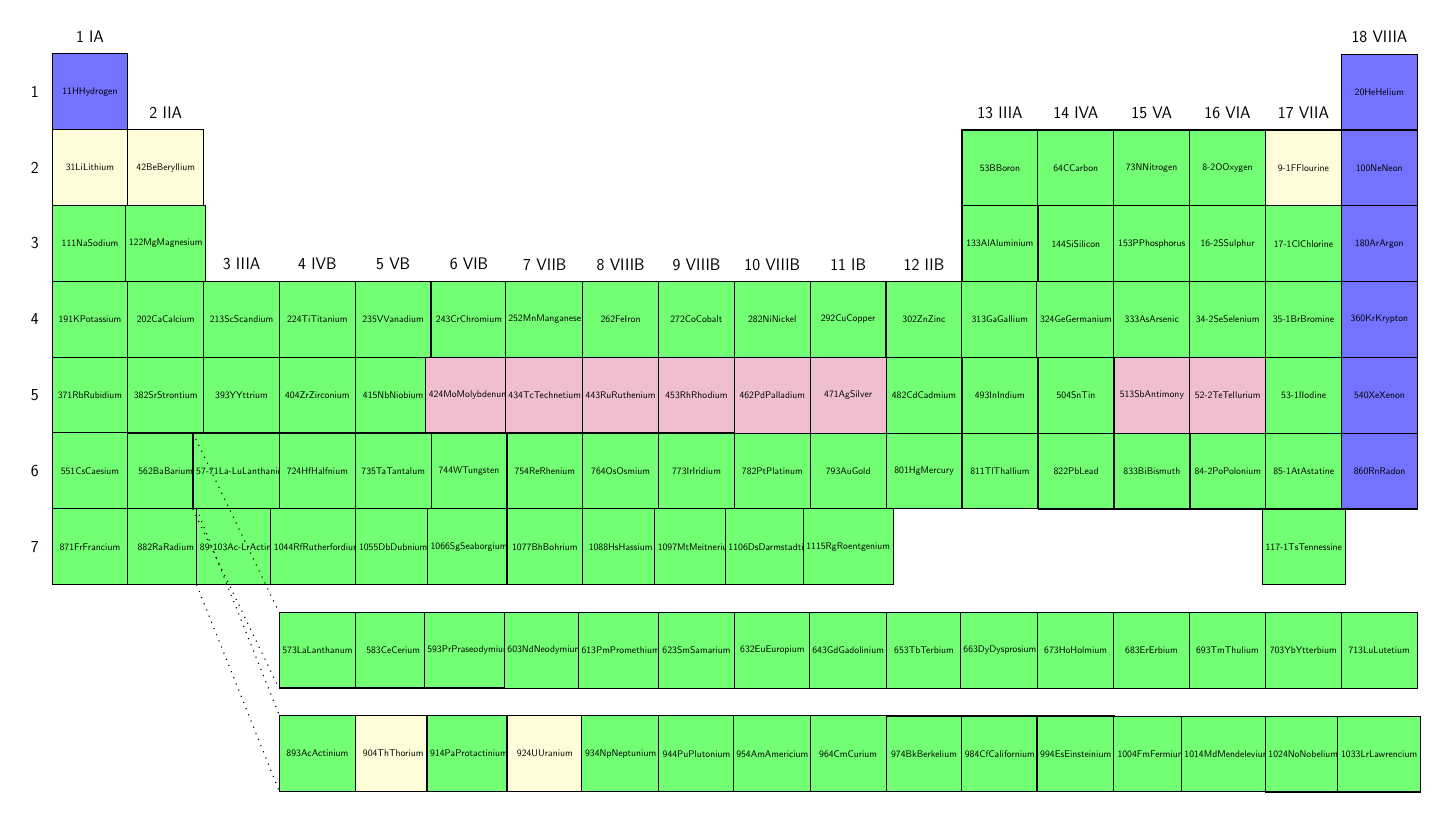
\begin{tikzpicture}[font=\sffamily, scale=0.35, transform shape]

%% Fill Color Styles
  \tikzstyle{ElementFill} = [fill=yellow!15]
  \tikzstyle{AlkaliMetalFill} = [fill=green!55]
  \tikzstyle{AlkalineEarthMetalFill} = [fill=green!55]
  \tikzstyle{MetalFill} = [fill=green!55]
  \tikzstyle{MetalloidFill} = [fill=green!55]
  \tikzstyle{NonmetalFill} = [fill=green!55]
  \tikzstyle{HalogenFill} = [fill=green!55]
  \tikzstyle{NobleGasFill} = [fill=green!55]
  \tikzstyle{LanthanideActinideFill} = [fill=green!55]
  \tikzstyle{B} = [fill=blue!55]
  \tikzstyle{N} = [fill=purple!25]
  \tikzstyle{F} = [fill=green!55]

%% Element Styles
  \tikzstyle{Element} = [draw=black, ElementFill,
    minimum width=2.75cm, minimum height=2.75cm, node distance=2.75cm]
  \tikzstyle{AlkaliMetal} = [Element, AlkaliMetalFill]
  \tikzstyle{AlkalineEarthMetal} = [Element, AlkalineEarthMetalFill]
  \tikzstyle{Metal} = [Element, MetalFill]
  \tikzstyle{Metalloid} = [Element, MetalloidFill]
  \tikzstyle{Nonmetal} = [Element, NonmetalFill]
  \tikzstyle{Halogen} = [Element, HalogenFill]
  \tikzstyle{NobleGas} = [Element, NobleGasFill]
  \tikzstyle{LanthanideActinide} = [Element, LanthanideActinideFill]
  \tikzstyle{PeriodLabel} = [font={\sffamily\LARGE}, node distance=2.0cm]
  \tikzstyle{GroupLabel} = [font={\sffamily\LARGE}, minimum width=2.75cm, node distance=2.0cm]
  \tikzstyle{TitleLabel} = [font={\sffamily\Huge\bfseries}]
  \tikzstyle{b} = [Element, B]
  \tikzstyle{n} = [Element, N]
  \tikzstyle{f} = [Element, F]

%% Group 1 - IA
  \node[name=H, b] {\NaturalElementTextFormat{1}{1}{H}{Hydrogen}};
  \node[name=Li, below of=H, Element] {\NaturalElementTextFormat{3}{1}{Li}{Lithium}};
  \node[name=Na, below of=Li, AlkaliMetal] {\NaturalElementTextFormat{11}{1}{Na}{Sodium}};
  \node[name=K, below of=Na, AlkaliMetal] {\NaturalElementTextFormat{19}{1}{K}{Potassium}};
  \node[name=Rb, below of=K, AlkaliMetal] {\NaturalElementTextFormat{37}{1}{Rb}{Rubidium}};
  \node[name=Cs, below of=Rb, AlkaliMetal] {\NaturalElementTextFormat{55}{1}{Cs}{Caesium}};
  \node[name=Fr, below of=Cs, AlkaliMetal] {\NaturalElementTextFormat{87}{1}{Fr}{Francium}};

%% Group 2 - IIA
  \node[name=Be, right of=Li, Element] {\NaturalElementTextFormat{4}{2}{Be}{Beryllium}};
  \node[name=Mg, below of=Be, AlkalineEarthMetal] {\NaturalElementTextFormat{12}{2}{Mg}{Magnesium}};
  \node[name=Ca, below of=Mg, AlkalineEarthMetal] {\NaturalElementTextFormat{20}{2}{Ca}{Calcium}};
  \node[name=Sr, below of=Ca, AlkalineEarthMetal] {\NaturalElementTextFormat{38}{2}{Sr}{Strontium}};
  \node[name=Ba, below of=Sr, AlkalineEarthMetal] {\NaturalElementTextFormat{56}{2}{Ba}{Barium}};
  \node[name=Ra, below of=Ba, AlkalineEarthMetal] {\NaturalElementTextFormat{88}{2}{Ra}{Radium}};

%% Group 3 - IIIB
  \node[name=Sc, right of=Ca, Metal] {\NaturalElementTextFormat{21}{3}{Sc}{Scandium}};
  \node[name=Y, below of=Sc, Metal] {\NaturalElementTextFormat{39}{3}{Y}{Yttrium}};
  \node[name=LaLu, below of=Y, LanthanideActinide] {\NaturalElementTextFormat{57-71}{}{La-Lu}{Lanthanide}};
  \node[name=AcLr, below of=LaLu, LanthanideActinide] {\NaturalElementTextFormat{89-103}{}{Ac-Lr}{Actinide}};

%% Group 4 - IVB
  \node[name=Ti, right of=Sc, Metal] {\NaturalElementTextFormat{22}{4}{Ti}{Titanium}};
  \node[name=Zr, below of=Ti, Metal] {\NaturalElementTextFormat{40}{4}{Zr}{Zirconium}};
  \node[name=Hf, below of=Zr, Metal] {\NaturalElementTextFormat{72}{4}{Hf}{Halfnium}};
  \node[name=Rf, below of=Hf, Metal] {\SyntheticElementTextFormat{104}{4}{Rf}{Rutherfordium}};

%% Group 5 - VB
  \node[name=V, right of=Ti, Metal] {\NaturalElementTextFormat{23}{5}{V}{Vanadium}};
  \node[name=Nb, below of=V, Metal] {\NaturalElementTextFormat{41}{5}{Nb}{Niobium}};
  \node[name=Ta, below of=Nb, Metal] {\NaturalElementTextFormat{73}{5}{Ta}{Tantalum}};
  \node[name=Db, below of=Ta, Metal] {\SyntheticElementTextFormat{105}{5}{Db}{Dubnium}};

%% Group 6 - VIB
  \node[name=Cr, right of=V, Metal] {\NaturalElementTextFormat{24}{3}{Cr}{Chromium}};
  \node[name=Mo, below of=Cr, n] {\NaturalElementTextFormat{42}{4}{Mo}{Molybdenum}};
  \node[name=W, below of=Mo, Metal] {\NaturalElementTextFormat{74}{4}{W}{Tungsten}};
  \node[name=Sg, below of=W, Metal] {\SyntheticElementTextFormat{106}{6}{Sg}{Seaborgium}};

%% Group 7 - VIIB
  \node[name=Mn, right of=Cr, Metal] {\NaturalElementTextFormat{25}{2}{Mn}{Manganese}};
  \node[name=Tc, below of=Mn, n] {\NaturalElementTextFormat{43}{4}{Tc}{Technetium}};
  \node[name=Re, below of=Tc, Metal] {\NaturalElementTextFormat{75}{4}{Re}{Rhenium}};
  \node[name=Bh, below of=Re, Metal] {\SyntheticElementTextFormat{107}{7}{Bh}{Bohrium}};

%% Group 8 - VIIIB
  \node[name=Fe, right of=Mn, Metal] {\NaturalElementTextFormat{26}{2}{Fe}{Iron}};
  \node[name=Ru, below of=Fe, n] {\NaturalElementTextFormat{44}{3}{Ru}{Ruthenium}};
  \node[name=Os, below of=Ru, Metal] {\NaturalElementTextFormat{76}{4}{Os}{Osmium}};
  \node[name=Hs, below of=Os, Metal] {\SyntheticElementTextFormat{108}{8}{Hs}{Hassium}};

%% Group 9 - VIIIB
  \node[name=Co, right of=Fe, Metal] {\NaturalElementTextFormat{27}{2}{Co}{Cobalt}};
  \node[name=Rh, below of=Co, n] {\NaturalElementTextFormat{45}{3}{Rh}{Rhodium}};
  \node[name=Ir, below of=Rh, Metal] {\NaturalElementTextFormat{77}{3}{Ir}{Iridium}};
  \node[name=Mt, below of=Ir, Metal] {\SyntheticElementTextFormat{109}{7}{Mt}{Meitnerium}};

%% Group 10 - VIIIB
  \node[name=Ni, right of=Co, Metal] {\NaturalElementTextFormat{28}{2}{Ni}{Nickel}};
  \node[name=Pd, below of=Ni, n] {\NaturalElementTextFormat{46}{2}{Pd}{Palladium}};
  \node[name=Pt, below of=Pd, Metal] {\NaturalElementTextFormat{78}{2}{Pt}{Platinum}};
  \node[name=Ds, below of=Pt, Metal] {\SyntheticElementTextFormat{110}{6}{Ds}{Darmstadtium}};

%% Group 11 - IB
  \node[name=Cu, right of=Ni, Metal] {\NaturalElementTextFormat{29}{2}{Cu}{Copper}};
  \node[name=Ag, below of=Cu, n] {\NaturalElementTextFormat{47}{1}{Ag}{Silver}};
  \node[name=Au, below of=Ag, Metal] {\NaturalElementTextFormat{79}{3}{Au}{Gold}};
  \node[name=Rg, below of=Au, Metal] {\SyntheticElementTextFormat{111}{5}{Rg}{Roentgenium}};

%% Group 12 - IIB
  \node[name=Zn, right of=Cu, Metal] {\NaturalElementTextFormat{30}{2}{Zn}{Zinc}};
  \node[name=Cd, below of=Zn, Metal] {\NaturalElementTextFormat{48}{2}{Cd}{Cadmium}};
  \node[name=Hg, below of=Cd, Metal] {\NaturalElementTextFormat{80}{1}{Hg}{Mercury}};

%% Group 13 - IIIA
  \node[name=Ga, right of=Zn, Metal] {\NaturalElementTextFormat{31}{3}{Ga}{Gallium}};
  \node[name=Al, above of=Ga, Metal] {\NaturalElementTextFormat{13}{3}{Al}{Aluminium}};
  \node[name=B, above of=Al, Metalloid] {\NaturalElementTextFormat{5}{3}{B}{Boron}};
  \node[name=In, below of=Ga, Metal] {\NaturalElementTextFormat{49}{3}{In}{Indium}};
  \node[name=Tl, below of=In, Metal] {\NaturalElementTextFormat{81}{1}{Tl}{Thallium}};

%% Group 14 - IVA
  \node[name=C, right of=B, Nonmetal] {\NaturalElementTextFormat{6}{4}{C}{Carbon}};
  \node[name=Si, below of=C, Metalloid] {\NaturalElementTextFormat{14}{4}{Si}{Silicon}};
  \node[name=Ge, below of=Si, Metalloid] {\NaturalElementTextFormat{32}{4}{Ge}{Germanium}};
  \node[name=Sn, below of=Ge, Metal] {\NaturalElementTextFormat{50}{4}{Sn}{Tin}};
  \node[name=Pb, below of=Sn, Metal] {\NaturalElementTextFormat{82}{2}{Pb}{Lead}};

%% Group 15 - VA
  \node[name=N, right of=C, Nonmetal] {\NaturalElementTextFormat{7}{3}{N}{Nitrogen}};
  \node[name=P, below of=N, Nonmetal] {\NaturalElementTextFormat{15}{3}{P}{Phosphorus}};
  \node[name=As, below of=P, Metalloid] {\NaturalElementTextFormat{33}{3}{As}{Arsenic}};
  \node[name=Sb, below of=As, n] {\NaturalElementTextFormat{51}{3}{Sb}{Antimony}};
  \node[name=Bi, below of=Sb, Metal] {\NaturalElementTextFormat{83}{3}{Bi}{Bismuth}};

%% Group 16 - VIA
  \node[name=O, right of=N, Nonmetal] {\NaturalElementTextFormat{8}{-2}{O}{Oxygen}};
  \node[name=S, below of=O, Nonmetal] {\NaturalElementTextFormat{16}{-2}{S}{Sulphur}};
  \node[name=Se, below of=S, Nonmetal] {\NaturalElementTextFormat{34}{-2}{Se}{Selenium}};
  \node[name=Te, below of=Se, n] {\NaturalElementTextFormat{52}{-2}{Te}{Tellurium}};
  \node[name=Po, below of=Te, Metalloid] {\NaturalElementTextFormat{84}{-2}{Po}{Polonium}};

%% Group 17 - VIIA
  \node[name=F, right of=O, Element] {\NaturalElementTextFormat{9}{-1}{F}{Flourine}};
  \node[name=Cl, below of=F, Halogen] {\NaturalElementTextFormat{17}{-1}{Cl}{Chlorine}};
  \node[name=Br, below of=Cl, Halogen] {\NaturalElementTextFormat{35}{-1}{Br}{Bromine}};
  \node[name=I, below of=Br, Halogen] {\NaturalElementTextFormat{53}{-1}{I}{Iodine}};
  \node[name=At, below of=I, Halogen] {\NaturalElementTextFormat{85}{-1}{At}{Astatine}};
  \node[name=Ts, below of=At, Halogen] {\SyntheticElementTextFormat{117}{-1}{Ts}{Tennessine}}; 

%% Group 18 - VIIIA
  \node[name=Ne, right of=F, b] {\NaturalElementTextFormat{10}{0}{Ne}{Neon}};
  \node[name=He, above of=Ne, b] {\NaturalElementTextFormat{2}{0}{He}{Helium}};
  \node[name=Ar, below of=Ne, b] {\NaturalElementTextFormat{18}{0}{Ar}{Argon}};
  \node[name=Kr, below of=Ar, b] {\NaturalElementTextFormat{36}{0}{Kr}{Krypton}};
  \node[name=Xe, below of=Kr, b] {\NaturalElementTextFormat{54}{0}{Xe}{Xenon}};
  \node[name=Rn, below of=Xe, b] {\NaturalElementTextFormat{86}{0}{Rn}{Radon}};

%% Period
  \node[name=Period1, left of=H, PeriodLabel] {1};
  \node[name=Period2, left of=Li, PeriodLabel] {2};
  \node[name=Period3, left of=Na, PeriodLabel] {3}; 
  \node[name=Period4, left of=K, PeriodLabel] {4}; 
  \node[name=Period5, left of=Rb, PeriodLabel] {5};
  \node[name=Period6, left of=Cs, PeriodLabel] {6};
  \node[name=Period7, left of=Fr, PeriodLabel] {7};

%% Group
  \node[name=Group1, above of=H, GroupLabel] {1 \hfill IA};
  \node[name=Group2, above of=Be, GroupLabel] {2 \hfill IIA};
  \node[name=Group3, above of=Sc, GroupLabel] {3 \hfill IIIA};
  \node[name=Group4, above of=Ti, GroupLabel] {4 \hfill IVB};
  \node[name=Group5, above of=V, GroupLabel] {5 \hfill VB};
  \node[name=Group6, above of=Cr, GroupLabel] {6 \hfill VIB};
  \node[name=Group7, above of=Mn, GroupLabel] {7 \hfill VIIB};
  \node[name=Group8, above of=Fe, GroupLabel] {8 \hfill VIIIB};
  \node[name=Group9, above of=Co, GroupLabel] {9 \hfill VIIIB};
  \node[name=Group10, above of=Ni, GroupLabel] {10 \hfill VIIIB};
  \node[name=Group11, above of=Cu, GroupLabel] {11 \hfill IB};
  \node[name=Group12, above of=Zn, GroupLabel] {12 \hfill IIB};
  \node[name=Group13, above of=B, GroupLabel] {13 \hfill IIIA};
  \node[name=Group14, above of=C, GroupLabel] {14 \hfill IVA};
  \node[name=Group15, above of=N, GroupLabel] {15 \hfill VA};
  \node[name=Group16, above of=O, GroupLabel] {16 \hfill VIA};
  \node[name=Group17, above of=F, GroupLabel] {17 \hfill VIIA};
  \node[name=Group18, above of=He, GroupLabel] {18 \hfill VIIIA};

%% Lanthanide
  \node[name=La, below of=Rf, LanthanideActinide, yshift=-1cm] {\NaturalElementTextFormat{57}{3}{La}{Lanthanum}};
  \node[name=Ce, right of=La, LanthanideActinide] {\NaturalElementTextFormat{58}{3}{Ce}{Cerium}};
  \node[name=Pr, right of=Ce, LanthanideActinide] {\NaturalElementTextFormat{59}{3}{Pr}{Praseodymium}};
  \node[name=Nd, right of=Pr, LanthanideActinide] {\NaturalElementTextFormat{60}{3}{Nd}{Neodymium}};
  \node[name=Pm, right of=Nd, LanthanideActinide] {\NaturalElementTextFormat{61}{3}{Pm}{Promethium}};
  \node[name=Sm, right of=Pm, LanthanideActinide] {\NaturalElementTextFormat{62}{3}{Sm}{Samarium}};
  \node[name=Eu, right of=Sm, LanthanideActinide] {\NaturalElementTextFormat{63}{2}{Eu}{Europium}};
  \node[name=Gd, right of=Eu, LanthanideActinide] {\NaturalElementTextFormat{64}{3}{Gd}{Gadolinium}};
  \node[name=Tb, right of=Gd, LanthanideActinide] {\NaturalElementTextFormat{65}{3}{Tb}{Terbium}};
  \node[name=Dy, right of=Tb, LanthanideActinide] {\NaturalElementTextFormat{66}{3}{Dy}{Dysprosium}};
  \node[name=Ho, right of=Dy, LanthanideActinide] {\NaturalElementTextFormat{67}{3}{Ho}{Holmium}};
  \node[name=Er, right of=Ho, LanthanideActinide] {\NaturalElementTextFormat{68}{3}{Er}{Erbium}};
  \node[name=Tm, right of=Er, LanthanideActinide] {\NaturalElementTextFormat{69}{3}{Tm}{Thulium}};
  \node[name=Yb, right of=Tm, LanthanideActinide] {\NaturalElementTextFormat{70}{3}{Yb}{Ytterbium}};
  \node[name=Lu, right of=Yb, LanthanideActinide] {\NaturalElementTextFormat{71}{3}{Lu}{Lutetium}};

%% Actinide
  \node[name=Ac, below of=La, LanthanideActinide, yshift=-1cm] {\NaturalElementTextFormat{89}{3}{Ac}{Actinium}};
  \node[name=Th, right of=Ac, Element] {\NaturalElementTextFormat{90}{4}{Th}{Thorium}};
  \node[name=Pa, right of=Th, LanthanideActinide] {\NaturalElementTextFormat{91}{4}{Pa}{Protactinium}};
  \node[name=U, right of=Pa, Element] {\NaturalElementTextFormat{92}{4}{U}{Uranium}};
  \node[name=Np, right of=U, LanthanideActinide] {\SyntheticElementTextFormat{93}{4}{Np}{Neptunium}};
  \node[name=Pu, right of=Np, LanthanideActinide] {\SyntheticElementTextFormat{94}{4}{Pu}{Plutonium}};
  \node[name=Am, right of=Pu, LanthanideActinide] {\SyntheticElementTextFormat{95}{4}{Am}{Americium}};
  \node[name=Cm, right of=Am, LanthanideActinide] {\SyntheticElementTextFormat{96}{4}{Cm}{Curium}};
  \node[name=Bk, right of=Cm, LanthanideActinide] {\SyntheticElementTextFormat{97}{4}{Bk}{Berkelium}};
  \node[name=Cf, right of=Bk, LanthanideActinide] {\SyntheticElementTextFormat{98}{4}{Cf}{Californium}};
  \node[name=Es, right of=Cf, LanthanideActinide] {\SyntheticElementTextFormat{99}{4}{Es}{Einsteinium}};
  \node[name=Fm, right of=Es, LanthanideActinide] {\SyntheticElementTextFormat{100}{4}{Fm}{Fermium}};
  \node[name=Md, right of=Fm, LanthanideActinide] {\SyntheticElementTextFormat{101}{4}{Md}{Mendelevium}};
  \node[name=No, right of=Md, LanthanideActinide] {\SyntheticElementTextFormat{102}{4}{No}{Nobelium}};
  \node[name=Lr, right of=No, LanthanideActinide] {\SyntheticElementTextFormat{103}{3}{Lr}{Lawrencium}};

%% Draw dotted lines connecting Lanthanide breakout to main table
  \draw (LaLu.north west) edge[dotted] (La.north west)
   %     (LaLu.north east) edge[dotted] (Lu.north east)
        (LaLu.south west) edge[dotted] (La.south west);
   %     (LaLu.south east) edge[dotted] (Lu.south east);
%% Draw dotted lines connecting Actinide breakout to main table
  \draw (AcLr.north west) edge[dotted] (Ac.north west)
   %     (AcLr.north east) edge[dotted] (Lr.north east)
        (AcLr.south west) edge[dotted] (Ac.south west);
   %     (AcLr.south east) edge[dotted] (Lr.south east);

\end{tikzpicture}
\end{centering}
\caption{Elements in blue are those which bubble out of the salt and are
included in the natural processes removal stream as are elements in light-red
as these are the `noble' metals which are insoluble in the salt. Elements in
green are considered fission products of which 50\% are removed every ten
years. Periodic table layout in TikZ provided by Chris Rump and Ivan Griffin
through overleaf.com}
\end{figure}

\subsection{Simulation Outputs}\label{ssec:outputs}

In Figures \ref{fig:fuel} through \ref{fig:k} the results of the simulation
described in section \ref{ssec:setup} - with input given in chapter 
\ref{ssec:input} - are given below. Following these figures in section
\ref{ssec:disc} the lessons learned from these figures and outputs are
given. The units given for group and stream values, $\%-\rho^{mat}_{i}$, are
relative fractions of the host material, $mat$, density as measured at the 
beginning of burnup step $i$.

\begin{figure}[H]
    \centering
    \includegraphics[width=0.8\textwidth]{fuel}
    \caption{The primary fuel constituents - Li (yellow), Be (purple), F (red),
    U (green), Th (blue) - atom density over the entire simulation.}
    \label{fig:fuel}
\end{figure}

\begin{figure}[H]
    \centering
    \includegraphics[width=0.8\textwidth]{fp}
    \caption{As described in section \ref{ssec:setup} and visually seen in
    Figure 3.1 here is seen the atomic density of all elements
    in the salt considered to be fission products.}
    \label{fig:fp}
\end{figure}

\begin{figure}[H]
    \centering
    \includegraphics[width=0.8\textwidth]{nat}
    \caption{The atomic density of the sum total of elements removed from the
    system by the stream used to simulate natural removal processes.}
    \label{fig:nat}
\end{figure}

\begin{figure}[H]
    \centering
    \includegraphics[width=0.8\textwidth]{proc}
    \caption{The atomic density of the sum total of elements removed from the
    system by the stream used to simulate a reprocessing function applied to
    the fuel salt.}
    \label{fig:proc}
\end{figure}

\begin{figure}[H]
    \centering
    \includegraphics[width=0.8\textwidth]{GgLiS}
    \caption{The atomic density of lithium elements considered to be a primary
    salt constituent.}
    \label{fig:GgLiS}
\end{figure}

\begin{figure}[H]
    \centering
    \includegraphics[width=0.8\textwidth]{GgLi}
    \caption{The atomic density of lithium elements excepting those considered 
    to be a primary salt constituent.}
    \label{fig:GgLi}
\end{figure}

\begin{figure}[H]
    \centering
    \includegraphics[width=0.8\textwidth]{GgAllLi}
    \caption{The atomic density of all lithium isotopes in the simulation.} 
    \label{fig:GgAllLi}
\end{figure}

\begin{figure}[H]
    \centering
    \includegraphics[width=0.8\textwidth]{GgBe}
    \caption{The atomic density of all beryllium isotopes in the simulation.} 
    \label{fig:GgBe}
\end{figure}

\begin{figure}[H]
    \centering
    \includegraphics[width=0.8\textwidth]{GgAllF}
    \caption{The atomic density of all fluorine isotopes in the simulation.} 
    \label{fig:GgAllF}
\end{figure}

\begin{figure}[H]
    \centering
    \includegraphics[width=0.8\textwidth]{GgFli}
    \caption{The atomic density of all fluorine isotopes considered to be bonded
    to lithium atoms which are considered to be primary fuel salt constituents.}
    \label{fig:GgFli}
\end{figure}

\begin{figure}[H]
    \centering
    \includegraphics[width=0.8\textwidth]{GgFbe}
    \caption{The atomic density of all fluorine isotopes considered to be bonded
    to beryllium atoms.}
    \label{fig:GgFbe}
\end{figure}

\begin{figure}[H]
    \centering
    \includegraphics[width=0.8\textwidth]{GgFth}
    \caption{The atomic density of all fluorine isotopes considered to be bonded
    to thorium atoms}
    \label{fig:GgFth}
\end{figure}

\begin{figure}[H]
    \centering
    \includegraphics[width=0.8\textwidth]{GgFu}
    \caption{The atomic density of all fluorine isotopes considered to be bonded
    to uranium atoms}
    \label{fig:GgFu}
\end{figure}

\begin{figure}[H]
    \centering
    \includegraphics[width=0.8\textwidth]{SgLii}
    \caption{The deposition rate integrated over the time of burnup step $i$
    for the stream injecting lithium isotopes into the system.}
    \label{fig:SgLii}
\end{figure}

\begin{figure}[H]
    \centering
    \includegraphics[width=0.8\textwidth]{SgLiFo}
    \caption{The removal rate integrated over the time of burnup step $i$
    for the stream removing \ce{LiF} from the system.}
    \label{fig:SgLiFo}
\end{figure}

\begin{figure}[H]
    \centering
    \includegraphics[width=0.8\textwidth]{SgBei}
    \caption{The deposition rate integrated over the time of burnup step $i$
    for the stream injecting beryllium-9 into the system.}
    \label{fig:SgBei}
\end{figure}

\begin{figure}[H]
    \centering
    \includegraphics[width=0.8\textwidth]{SgBeF2o}
    \caption{The removal rate integrated over the time of burnup step $i$
    for the stream removing \ce{BeF2} from the system.}
    \label{fig:SgBeF2o}
\end{figure}

\begin{figure}[H]
    \centering
    \includegraphics[width=0.8\textwidth]{SgFi}
    \caption{The deposition rate integrated over the time of burnup step $i$
    for the stream injecting fluorine-19 into the system.}
    \label{fig:SgFi}
\end{figure}

\begin{figure}[H]
    \centering
    \includegraphics[width=0.8\textwidth]{SgFo}
    \caption{The removal rate integrated over the time of burnup step $i$
    for the stream removing fluorine from the system.}
    \label{fig:SgFo}
\end{figure}

\begin{figure}[H]
    \centering
    \includegraphics[width=0.8\textwidth]{SgThF4i}
    \caption{The deposition rate integrated over the time of burnup step $i$
    for the stream injecting \ce{^{232}Th^{19}F4} into the system.}
    \label{fig:SgThF4i}
\end{figure}

\begin{figure}[H]
    \centering
    \includegraphics[width=0.8\textwidth]{SgThF4o}
    \caption{The removal rate integrated over the time of burnup step $i$
    for the stream removing \ce{^{232}Th^{19}F4} from the system.}
    \label{fig:SgThF4o}
\end{figure}

\begin{figure}[H]
    \centering
    \includegraphics[width=0.8\textwidth]{SgUF4i}
    \caption{The deposition rate integrated over the time of burnup step $i$
    for the stream injecting \ce{^{233}U^{19}F4} into the system.}
    \label{fig:SgUF4i}
\end{figure}

\begin{figure}[H]
    \centering
    \includegraphics[width=0.8\textwidth]{SgUF4o}
    \caption{The removal rate integrated over the time of burnup step $i$
    for the stream removing \ce{^{233}U^{19}F4} from the system.}
    \label{fig:SgUF4o}
\end{figure}

\begin{figure}[H]
    \centering
    \includegraphics[width=0.8\textwidth]{fluorine}
    \caption{The amount of fluorine over time in excess of the amount of 
    fluorine required to bind to all the primary salt constituents: 
    \ce{LiF}, \ce{BeF2}, \ce{ThF4}, \ce{UF4}.}
    \label{fig:fluroine}
\end{figure}

\begin{figure}[H]
    \centering
    \includegraphics[width=0.8\textwidth]{all_oxid}
    \caption{The simulation's summed oxidation state over all elements and
    weighted by the prevalence of that elements ,as in equation \ref{eq:oxi},
    over time.}
    \label{fig:all_oxid}
\end{figure}

\begin{figure}[H]
    \centering
    \includegraphics[width=0.8\textwidth]{k}
    \caption{The observed infinite neutron multiplication factor of the system
    complete with error. The very first time point at $t=0$ is excluded from
    this plot for scale reasons. The initial infinite neutron multiplication 
    factor of the system was approximately 1.5.}
    \label{fig:k}
\end{figure}

\begin{figure}[H]
    \centering
    \includegraphics[width=0.8\textwidth]{flux_0}
    \caption{The scalar neutron flux within the system broken up into
    equal-lethargy width bins taken at day zero.}
    \label{fig:flux_0}
\end{figure}

\begin{figure}[H]
    \centering
    \includegraphics[width=0.8\textwidth]{flux_219}
    \caption{The scalar neutron flux within the system broken up into
    equal-lethargy width bins taken at burnup step 219 - the center of the
    discontinuity.}
    \label{fig:flux_219}
\end{figure}

\begin{figure}[H]
    \centering
    \includegraphics[width=0.8\textwidth]{flux_601}
    \caption{The scalar neutron flux within the system broken up into
    equal-lethargy width bins taken after the last burnup step.}
    \label{fig:flux_601}
\end{figure}

\begin{figure}[H]
    \centering
    \includegraphics[width=0.8\textwidth]{Uf}
    \caption{The relative percentage change in the fission cross section of
    \ce{^{233}U} per burnup step throughout the simulation.}
    \label{fig:uf}
\end{figure}

\begin{figure}[H]
    \centering
    \includegraphics[width=0.8\textwidth]{Uc}
    \caption{The relative percentage change in the absorption cross section of
    \ce{^{233}U} per burnup step throughout the simulation.}
    \label{fig:uf}
\end{figure}

\subsection{Simulation Assessment}\label{sec:disc}

In Figure \ref{fig:fuel} the elemental salt constituent atomic
densities for Li, Be, F, Th, and U are plotted over time. This plot represents
a turning point in MSR modelling, one after which incorporating chemistry 
restraints into nuclear burnup calculations is possible. Beginning with fluorine
as the most abundant salt constituent a steady decline is observed - at first
very slight but growing in magnitude towards the end of the simulation. At an
exaggerated scale figure \ref{fig:GgAllF} magnifies this trend. 

Throughout this section a theme that will emerge are the apparent shortcomings
of using the CLP linear optimization library for such an endeavor. While Sandia
national labs tested CLP themselves, \cite{gearhart_comparison_2013}, and my
own stress tests as well as ADER's unit and integration tests confirmed that
CLP could and would handle the floating point precision involved in these kinds
of problems, it was not until years later that Ma and Saunders would show in
\cite{STANFORD} that the numerical instability issues do not arise until many
thousands of parameters are involved in the calculations. The input for this
simulation was checked in a debugger at every stage of program execution and was
found to be consistent with the expected behavior given the input seen in
chapter \ref{ch:input}. Indeed, the linear optimization matrix as requested by
CLP was checked and found to be consistent with describing the input to CLP.
Despite this the behavior from CLP, as observed in the previous figures, 
indicates a solutions which ignores arbitrary parameters as well as crashing
all together on a whole host of other problems.

A prime example of this behavior is seen in figure \ref{fig:SgFi} where the
injection stream for fluoride-19 is seen to take only negative values other than
zero. A hard lower bound of zero was applied to all streams in the CLP solution.
An interesting observation is that this 'negative injection' by this stream
would seem to fill in the missing trend seen in figure \ref{fig:SgFo} and indeed
accounts for some of the change observed in figure \ref{fig:GgAllF}. Figure
\ref{fig:SgFo} does have the expected behavior in reference to figure
\ref{fig:GgAllF}. While CLP ignores some parameters it does follow others as
exemplified in figure \ref{fig:fluorine} where it can be seen that throughout
the entire simulation sufficient fluorine was kept in the system to bind to all
primary fuel constituents where excess fluorine is taken to be the fluorine 
unaccounted for in the system after summing all fluorine required to bond to the
primary fuel constituents. Figures \ref{fig:GgF-li}, \ref{fig:GgF-be},
\ref{fig:GgF-th}, and \ref{fig:GgF-u} confirm that the respective fluorine
groups track their bonded element at the appropriate ratios.

The behavior seen for beryllium follows a similar trend with the removal stream
for \ce{BeF2} having negative values corresponding to a brief positive trend
in the injection stream for beryllium as can be seen in figures
\ref{fig:SgBeF2o} and \ref{fig:SgBei} respectively. This behavior is consistent
with the maximization for the beryllium fuel group by ADER in the initial days
of fission product production to counter the produced negative reactivity by
further thermalizing the spectrum with beryllium. 

This observation is further backed by the initial loss of lithium in the
early steps of the simulation as seen in figures \ref{fig:GgLiS} and 
\ref{fig:GgAllLi} - again to increase system reactivity as lithium-6 is a
strong neutron poison. Again slight negative values are seen in a stream as can
be observed in figure \ref{fig:SgLiFo}. The increased injections of lithium 
into the system, accounting for the rise seen in figure \ref{fig:GgAllF}, are
seen in figure \ref{fig:SgLii}. From figure \ref{fig:GgLi} it can be seen that
this increase in lithium was not for primary salt constituent balance purposes.
Rather, this increase in lithium, along with the expected increase in fission
products which are entirely oxidizing to the salt, accounts for the overall
system increase of the weighted oxidation state value as seen in figure
\ref{fig:all_oxid}.

This continued increase of the weighted system oxidation state up to the
positive asymptote observed at 0.004 a.u. is a complete violation of the 
hard oxidation state value limits that were set for this simulation of 
$[-0.0002, -0.0001]$. Furthermore it would seem that this system oxidation
state was actually pursued by CLP as there is no other reason to by injecting
additional lithium, a neutron poison, into the system.

The initial injections of thorium into the system as seen in figure
\ref{fig:SgThF4i} are produced to account for the unacceptably high 
initial system neutron multiplication factor as can be seen in figure
\ref{fig:k} - even though in that figure the very first point at $[k=1.06,t=0]$
has been cut off for scale readability purposes. Interestingly enough the
thorium removal stream maintains a perfect zero value throughout 
the simulation indicating that the thorium depletion seen in figure
\ref{fig:fuel} is due entirely to nuclear processes to the degree that would be
expected.

Looking to uranium the two errant values of positive uranium removal seen in
figure \ref{fig:SgUF4o} have no explanation other than possible CLP numerical
instability. On the other hand, the steady increase in uranium injection
as seen in figure \ref{fig:SgUF4i} is entirely expected given the observed
increase in fission products, a powerful neutron poison, in figure \ref{fig:fp}.

The behavior of the natural processes removal stream, as seen in figure
\ref{fig:nat} follows the expected pattern with a rapid rise to its
saturation value as the equilibrium content of short lived - or rapidly removed
- fission products is approached. The behavior of the reprocessing stream as 
seen in figure \ref{fig:proc} agrees with the behavior observed for the overall
fission product concentration as seen in figure \ref{fig:fp} and for which the
two of them explain the fission product concentration approach to its
equilibrium value.

In the first 6000 days of the simulation ADER maintains the neutron
multiplication factor within the requested bounds as seen in figure \ref{fig:k}
through the application of streams as seen in the figures previously 
discussed. However, over a series of burnup steps, 216 - 221, the
neutron multiplication factor of the system falls quickly, and then while
remaining below the desired neutron multiplication factor targets, continues
in a downward trend despite a continuing increase in the amount of \ce{^{233}U}
injected into the system as seen in figure \ref{fig:SgUF4i}. As seen in figures
\ref{fig:uf} and \ref{fig:uc} the fission and capture cross sections of 
\ce{^{233}U} do not change through the entire simulation. Furthermore, as
can be seen in figures \ref{fig:flux_0}, \ref{fig:flux_219}, and 
\ref{fig:flux_601} the neutron spectrum does not change through the entire 
simulation and not in the middle of the discontinuity either. In debugging
efforts no deviation from previous burnup steps or later burnup steps
in the evaluation of nuclear cross sections by ADER was found however ADER
consistently, from the discontinuity inwards, chose material configurations
that by its own calculations would drive the system neutron multiplication
factor below the desired minimum target of 1.00.

Overall these results represent a mixed bag. Obviously ADER's use of CLP suffers
from pernicious and extensive numerical instability issues. These issues
manifest not just in aborted simulations but in simulation results which 
do not adhere to the system parameters as defined. Despite these shortcomings
ADER does execute some of its intended functions such as general chemical
solubility control and species accounting. It is in the additional and single
row objectives that ADER seems to produce errant results. 
 

\chapter{Conclusions and Future Work}
\label{ch:conc}

In the last twenty years molten salt reactors have seen an incredible surge of
global attention as evidenced in such international programs as MOSART, ALISIA,
and the LF-TMSR out of China, as well as increased research attention as
evidenced by the continuing success of Oak Ridge National Laboratory's MSR
workshop which now averages over 400 attendees from across the globe yearly. 
While significant investment and progress has been made in nearly all aspects
of MSR development from material selection, salt purification and property
measurement, licensing and general reactor design, comparatively little
attention has been paid to fuel cycle analysis. The majority of attempts in
this area have fallen short of producing widely applicable results largely due
to the limiting effects of specific assumptions such as the salt species
involved or the coarseness of the solution. In this work a method and
implementation of a general approach for modelling and evaluating molten salt
reactor fuel cycles is proposed. This approach is based upon a linear
optimization routine designed to approximate the limitations of the chemistry
and nuclear concerns of reactor operations while optimizing the driving concerns
of the reactor operators. This approach, named ADER for the Advanced Depletion
Extension for Reprocessing, is built into the reactor physics Monte-Carlo code
SERPENT 2.  While the theory and algorithm are found to be
sound, the specific implementation has been discovered to suffer from
significant and deleterious numerical instability within the 
linear optimization solver.

In its present state the usefulness of ADER is concerningly compromised and
the implementation as a whole is drastically limited in the range of simulations
it can execute with no method a priori to establish feasibility. Any future
work going forth on this project would need to begin with the implementation
of a floating-point quadruple-precision linear optimization solver in the place
of the current CLP implementation. Following such a development it is expected
that ADER will be capable of simulating the wide variety of parameters which its
input and structure allow. Additional improvements could be found through the
incorporation of an iteration scheme whereupon the effects of nuclear burnup
on the isotopics of the fuel over a burnup step can be approximated as a
proportional removal stream on the whole system in the linear optimization
scheme such that the approximated total effects of nuclear burnup are considered
in material optimization. Additional improvements may be found in abandoning the
linear optimization solver all together and rather moving towards a gradient
approach from which an iteration scheme to more closely approximate the 
effects of streams on nuclear criticality could be arrived at. 

Overall the impact of ADER is unclear and will only be known in the future.
Given ADER's extensive test suite, documentation, and modular construction, it
is not unimaginable that the above mentioned improvements may one day be made.
In such a future the impact of ADER would certainly be greater than it is today.
Despite this shortcoming ADER has shown that a linear optimization scheme can
be effectively applied to the chemistry, nuclear, and operational concerns of a
molten salt reactor in such a way as to predict the future fuel composition and 
nuclear characteristics of the system.


\def\StripPrefix#1>{}
\def\jobis#1{FF\fi
  \def\predicate{#1}%
  \edef\predicate{\expandafter\StripPrefix\meaning\predicate}%
  \edef\job{\jobname}%
  \ifx\job\predicate
}

\if\jobis{thesis}
  \printbibliography
\else
  \newpage
  \renewcommand{\thepage}{}
  \printbibliography
\fi

%\appendix
% \include{mathbg}

\end{document}
